\documentclass[acmlarge]{acmart}

\usepackage[ruled]{algorithm2e} % For algorithms
\usepackage{balance}       % to better equalize the last page
\usepackage{graphics}      % for EPS, load graphicx instead
\usepackage[T1]{fontenc}   % for umlauts and other diaeresis
\usepackage{txfonts}
\usepackage{mathptmx}
\usepackage{booktabs}
\usepackage{textcomp}
\usepackage{microtype}        % Improved Tracking and Kerning
\usepackage{ccicons}          % Cite your images correctly!
\usepackage{mathrsfs}
\usepackage{subfigure}
\usepackage{multirow}
\usepackage{xspace}
\usepackage{enumitem}
\usepackage{rotating}
\usepackage{caption}
\usepackage{tabularx}
\usepackage{color}

\newtheorem{theorem}{Theorem}
\newcommand{\systemname}{\textsc{SleepGuard}\xspace}

\renewcommand{\algorithmcfname}{ALGORITHM}
\SetAlFnt{\small} \SetAlCapFnt{\small} \SetAlCapNameFnt{\small} \SetAlCapHSkip{0pt} \IncMargin{-\parindent}

% Metadata Information
\acmJournal{IMWUT} \acmVolume{9} \acmNumber{4} \acmArticle{39} \acmYear{2018} \acmMonth{3} \acmArticleSeq{11}
% Copyright
\setcopyright{acmcopyright}
%\setcopyright{acmlicensed}
%\setcopyright{rightsretained}
%\setcopyright{usgov}
%\setcopyright{usgovmixed}
%\setcopyright{cagov}
%\setcopyright{cagovmixed}

% DOI
\acmDOI{0000001.0000001}
% Paper history
\received{February 2018} \received{March 2018} \received[accepted]{June 2018}



\newcommand{\red}[1]{\textcolor{red}{#1}}
\newcommand{\blue}[1]{\textcolor{blue}{#1}}
\newcommand{\yellow}[1]{\textcolor{yellow}{#1}}
\newcommand{\green}[1]{\textcolor{green}{#1}}
\newcommand{\cyan}[1]{\textcolor{cyan}{#1}}
\newcommand{\brown}[1]{\textcolor{brown}{#1}}
\newcommand{\purple}[1]{\textcolor{purple}{#1}}
\newcommand{\orange}[1]{\textcolor{orange}{#1}}

\newcommand{\etal}{\emph{et al.}}


\begin{document}

\title{Tracking Rich Sleep Events Using Smartwatch Sensing Data}

\author{Liqiong Chang, Jiaqi Lu, Ju Wang, Xiaojiang Chen, Dingyi Fang, Zhanyong Tang}
\orcid{1234-5678-9012-3456}
\affiliation{
	\institution{Northwest University}
	\country{China}} \email{{changliqiong, jlh, xjchen, dyf, zytang}@nwu.edu.cn}

\author{Petteri Nurmi, Zheng Wang}
\affiliation{
	\institution{Lancaster University}
	\country{United Kingdom}} \email{{p.nurmi, z.wang}@lancaster.ac.uk}



\begin{abstract}
Sleep is an important part of our daily routine -- we spend about one-third of our time doing it. By tracking the sleep-related events
and activities, sleep monitoring provides the decision support to help us understand the sleep quality and the causes of poor sleep.
Wearable devices provide a new way for sleep monitoring, allowing us to monitor sleep from the comfort of our own home, but existing
solutions do not take full advantage of the rich sensor data provided by these portable devices. In this paper, we develop a novel
approach to track a wide range of sleep-related events using smartwatches. We show that it is possible to track, using a single
smartwatch, sleep events like body postures and movements, acoustic events, and illumination conditions. From these events, a statistical
model can be designed to effectively evaluate a user's sleep quality across various sleep stages. We evaluate our approach by conducting
extensive experiments involved ten users across a 2-week period. Our experimental results show that our approach can track a richer set
of sleep events, which provides better decision support for evaluating the sleep quality, when compared to prior work.
\end{abstract}


\begin{CCSXML}
	<ccs2012>
	<concept>
	<concept_id>10003120.10003138</concept_id>
	<concept_desc>Human-centered computing~Ubiquitous and mobile computing</concept_desc>
	<concept_significance>500</concept_significance>
	</concept>
	</ccs2012>
\end{CCSXML}

\ccsdesc[500]{Human-centered computing~Ubiquitous and mobile computing}

\keywords{Smartwatch, Sleep events, Sensing}

\thanks{This work is partially supported by the National Natural Science Foundation of China under Grant Nos. 61572402, 61672428, 61772422 and 61572347.}

\maketitle

\renewcommand{\shortauthors}{L. Chang, J. Lu, J. Wang, X. Chen, D. Fang, Z. Tang, Z. Wang, P. Nurmi}



\section{INTRODUCTION}\label{sec:1introduction}

Sleep plays a vital role in good health and well-being throughout a person's life. Lacking of sleep or having poor sleep can lead to
serious, sometimes life-threatening, health problems~\cite{lallukka2016contribution}. The quality of sleep depends on many factors,
including the sleeping environment such as the light intensity and the ambient temperature, the user's breath, the sleeping posture, and
the bedtime routine. By capturing and modeling these factors, sleep monitoring can help users to assess and understand their sleeping
pattern, and provide feedback on how the change of the sleeping environment and behavior affect the sleep quality.

Traditionally, sleep monitoring had to be done in a clinic environment using dedicated medical equipment.  Modern mobile devices such as
smartphones and smartwatches offer a new way for sleep monitoring. By utilizing the rich mobile sensors, we can track certain activities
such as body movements or snore, and to use the tracked information to detect and model sleep
patterns~\cite{zeo,Jawbone,SleepAndroid,fitbit,gu2016sleep}. Such an approach is known as
\emph{actigraphy}~\cite{Actigraphy,ancoli2003role}. An actigraphy approach has several advantages over a clinic solution, including being
lower cost and non-invasive, and can be performed at home on an on-going basis.

%like electroencephalography (EEG), \`{o}electrocardiography (ECG) and electromyography (EMG)

However, existing mobile-based sleep monitoring applications fail to fully exploit the sensors provided by modern mobile devices. As a
result, current mobile-based sleep monitoring system typically only provide superficial information such as the duration of deep and
shallow sleep. Without further detailed information of the environment and activities across sleep stages, these applications offer little
help in understanding the causes of poor sleep. To unlock the potential of mobile-based sleep monitoring, we need to find ways to take full
advantage of the rich sensor data provided by modern mobile devices.


The work presented by Gu \etal~\cite{gu2016sleep} is among the first attempts in this direction
\cite{lawson2013validating,bauer2012shuteye,min2014toss,al2014classifying}. Their work exploits smartphone sensors to detect physical and
acoustical activities happened during sleep. While promising, this approach requires placing the smartphone next to the user's head and
ensuring the phone remains stationary throughout the sleeping process. However, this requirement often cannot be satisfied and many users
do not want to place the mobile phone too close to the body due to health risk concerns~\cite{StepHealth,Quorasleep}.

\begin{figure}[!t]
\centering
\setlength{\belowcaptionskip}{-13pt}
      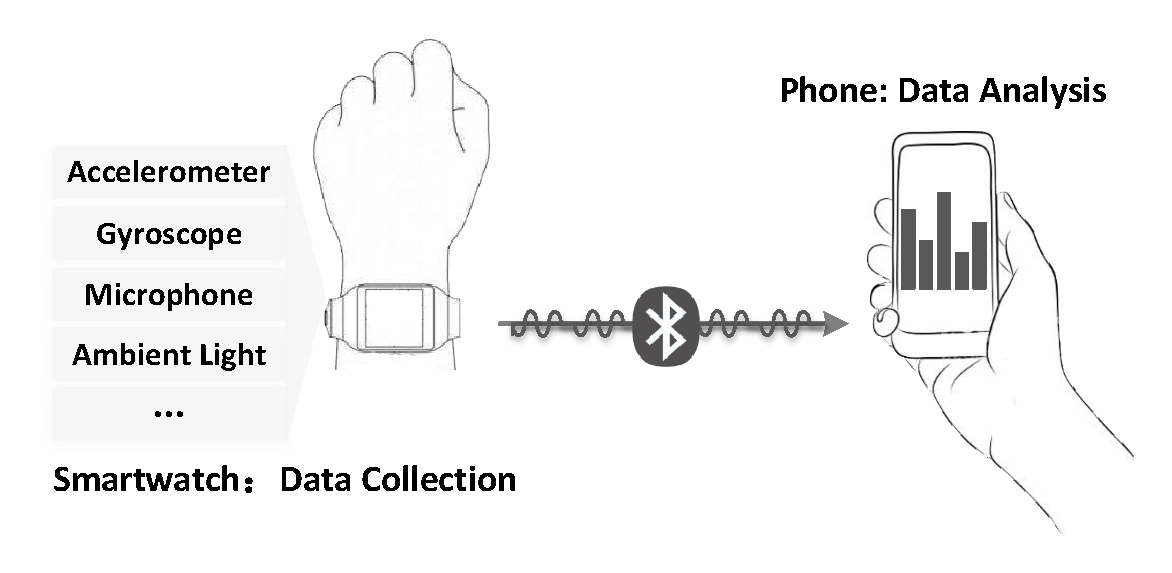
\includegraphics[width=0.5\textwidth]{Figures/datacollect.pdf}
  \caption{{\systemname} detects a wide range of sleep-related activities and events using a smartwatch.}\label{fig:datacollect}
\end{figure}

This paper presents a better approach. Instead of using smartphones and relying on strict, unrealistic assumptions, we exploit the rich
sensor data provided by smartwatches to track a wider range of sleep-related activities. The advantages of using a smartwatch are that
many users are willing to wear the device throughout the night, thus the device can remain relatively close to the user over the duration
of sleep.  The smartwatch also allows us to collect a richer set of information. The collected information can then be used to monitor a
wider range of sleep-related events. While there are prior works on sleep monitoring based on smartwathes
\cite{pombo2016ubisleep,shelgikar2016sleep,haescher2015anomaly,borazio2012combining}, these approaches only gather coarse-grained
information and often rely on specialize devices such as pressure mattresses or image acquisition equipment. In this work, we demonstrate
that, for the first time, smartwatches enable us to collect an extensive set of sleep-related events -- many of which are not supported in
prior work. Having a more comprehensive set of sleep-related events and activities will thus enable users to gain a deeper understanding of
their sleep patterns and the causes of poor sleep.



In this paper, we present \systemname, the first smartwatch-based monitoring system that can track a wide range of sleep-related
activities. \systemname gathers sleep-related activities by utilizing the commonly available sensors on smartwatches: the accelerometer,
gyroscope, microphone and ambient light sensor, etc. It then uses the tracked information to infer the user's sleep posture and habits --
thing like changes of body and hand positions, as well as sound events due to e.g. snoring or coughing.  Collecting these data can help a
user to gain a deep understanding of his/her sleeping pattern and quality, and to find ways to improve sleep.

However, translating the collected senor data to these sleeping events is non-trivial due to the changing nature of smartwatches during
sleep. To overcome these challenges, we develop a set of new methods and analysis, specifically targeting portable mobile devices.  The key
insight behinds {\systemname} is that the sleep quality is strongly correlated to the sleep posture, acoustic events and the illumination
condition \cite{shelgikar2016sleep}. By exploiting the unique characteristics of sensory data produced by different sleep activities, we
develop a series of novel algorithms to correlate the sensory data to sleep events. We then design a model to incorporate the detected
events to
infer the user's sleep stages and sleep quality.

We evaluate our approach by applying it to ten users over two weeks period. The experimental results show that {\systemname} is  effective
and accurate in capturing sleep-related activities. For body posture classification, body rollover recognition, hand position
identification and  acoustic events detection,  it achieves least accuracies of 98\%,  90\%,  87\% and  96.9\%, respectively. These results
show that {\systemname}  is superior to existing actigraphy-based applications.

Our main contributions are:

\begin{itemize}[itemsep=1mm,nolistsep]

\item We present a novel sleep monitoring system based on smartwatch sensor information. Our system captures a wider range of sleeping
    activities that none of the current mobile-based sleep monitoring solutions can offer.

\item We design a set of new algorithms and analysis to effectively exploit the smartwatch sensor data to detect sleep-related
    activities. These include body postures, body rollovers, hand positions, micro body movements and acoustical events.

\item The experimental results suggest that our prototype system, \systemname, is highly effective in capturing sleep-related events.

\end{itemize}

%ZW: I have commented out the motivation section as it reads like related work.
%\section{MOTIVATION}\label{Sec:motivation}
In this section, we will explain our system motivation. Sleep takes most of the time in a person's life, and a good sleep plays a very
important role throughout the day. Sleep can help people restore the body's function, store energy, and repair damaged cells. According to
medical reports, good sleep can make the body and mind get appropriate rest and conditioning, promote metabolism simultaneously. If the
lack of sleep time or poor sleep environment for a long time will cause mental malaise, inattention, and even life-threatening. So how to
create high sleep quality is essential and necessary. Therefore, to improve the quality of sleep, first of all, we should clarify the
factors that affect the quality of sleep. Then, we find a standard to assess the quality of sleep to help people improve sleep.

According to our survey, we can classify the factors that affect sleep quality into the following, which is why our system selects some of these events for detection.
\begin{itemize}
  \item Personal sleep habits: sleep habits include pre-sleep diet, sleeping posture, the hand position and so on. For diet, we should try to avoid eating sugary and fatty foods too much, it will change your blood sugar level, and then delay sleep \cite{eating2013,eating2014}. And sleeping posture should be paid more attention by us. According to research, dreaming and sleep quality are associated with underlying brain functions and may be affected by body posture \cite{posture2004}. It has been well stated that right-side sleepers had better subjective sleep quality than left-side sleepers. And for different people, they should have his own fit sleeping posture, taking into account his own physical factors \cite{posture2016,posture2017}. For example, people with ailments such as heart disease or high blood pressure are unfit for prone position. We can consciously avoid or take some kind of sleep posture, which will have very good benefits for your sleep quality and health \cite{posture2015}. Further, if a proper hand position isn't regulated and maintained, it can cause a massive array of problems for sleep \cite{position2014}. For example, if you get used to putting your hand on your head when you sleep, you will feel tingling and numbness. even after moving position, an underlying symptom may be the early stages of carpal tunnel syndrome. So in {\systemname}, we incorporate sleep position and hand position into the detection of events so that the factors that affect the quality of sleep can be more widely considered.
  \item sleep environment: the bedroom environment can have a significant influence on sleep. Both the light, noise, and temperature can be the culprit in poor sleep. We have found that too much light exposure can shift our biological clock , which makes restful sleep difficult to achieve, it affects our sleep and wake cycle \cite{light2007}. Besides, we also note that the dim light will affect our sleep too. According to the study \cite{light2016}, it can be learned that the dim artificial light during sleep is significantly associated with the general increase in fatigue. So the proper light can be used to increase the sense of exhaustion, thereby promoting sleep. As for noise, in order to promote better sleep, we need to reduce the volume of noise as much as possible. And the ideal temperature range for sleeping, there is no prescribed best standard among different individuals \cite{light2007}. So in {\systemname}, we mainly detect the illumination condition in the environment and make it as one of evaluation indicators for sleep quality.
  \item Physiological factors: physiological factors will have an impact on the structure and distribution of sleep. When the body is not comfort, such as cough, body aches, etc, the human cerebral cortex cells are always in an excited state, can not enter the inhibition and limit the depth of sleep and allow only brief episodes of sleep between awakenings, it like many other sleep disruptions. And long-term snoring can also have a serious impact on health and sleep. It can cause behind sleep apnea or narcolepsy, a sleeping disorder \cite{snoring2016,snoring2013}. However, Snoring is subject to many influences such as body position, sleep stage and the presence or absence of sleep-disordered breathing \cite{snoring2010}. So our system have taken the acoustic events during sleep into consideration, including snore,cough and somniloquy.
  \item Psychological factors: psychological factors are also one of the important reasons that affect the quality of sleep. During the daytime, people are mainly awakened by their daily activities. This is awakening. When people sleep at night, they mainly show up as a sleeping substance, which results in depression and sleep. If the excitement and inhibition can not maintain a certain balance to complete the awakening and sleep conversion, it will have insomnia and other symptoms. what's more, individuals of all ages who experience stress, anxiety, and depression tend to find it more difficult to fall asleep \cite{mood2003,light2007,mood2015}. For this factor, we can use the way of asking questions to record the user's psychological state before sleep
\end{itemize}

In addition to these events, we also considered the body rollover event during sleep, as turning over is also a necessary exercise during
sleep \cite{rollover2014,rollover201408}. We can get some reflections of sleep status by counting the number of body rollover during a
whole night. And we can understand the user's detailed sleep information by detecting  micro body movement (hand moving, arm raising, and
body trembling) during sleep.

According to our investigation, The quality of sleep is largely determined by the percentage of different sleep stages throughout the sleep
\cite{iSleep,gu2016sleep}, so we can segment the user's entire sleep process into sleep stages and calculate the proportion of each
sleeping stage in the whole sleep process, in order to assess the quality of sleep.  Sleep stage refers to the three main stages, namely
Rapid Eye Movement (also called dream stage), light sleep stage and deep sleep stage. The light sleep and deep sleep are also called
non-Rapid Eye Movement (NREM). And the division of the sleep stage is based on the fact that sleepers usually exhibit distinguishable
physical activities in different sleep stages \cite{ancoli2003role}. For example, body trembling and somniloquy often occur in REM while
large body movements and snoring are more prone to occur in the deep sleep stage, and the roll-over frequency can also help us to classify
the sleep stage \cite{rollover2007}. So we divide the sleep stage based on detecting these specific events  that belong to different stages
of sleep. In addition, the quality of sleep is also affected by age, sleep mate and other factors, we will further consider in future work.

%\textcolor{blue}{\section{SYSTEM OVERVIEW}}
In this section, we present the overview of {\systemname}. It is a system based on smartwatch that can recognize different sleep-related events and report the details. Three main modules are illustrated in Fig. \ref{fig:overview}.

\begin{figure}[!thbp]
\centering
%\setlength{\belowcaptionskip}{-9pt}
      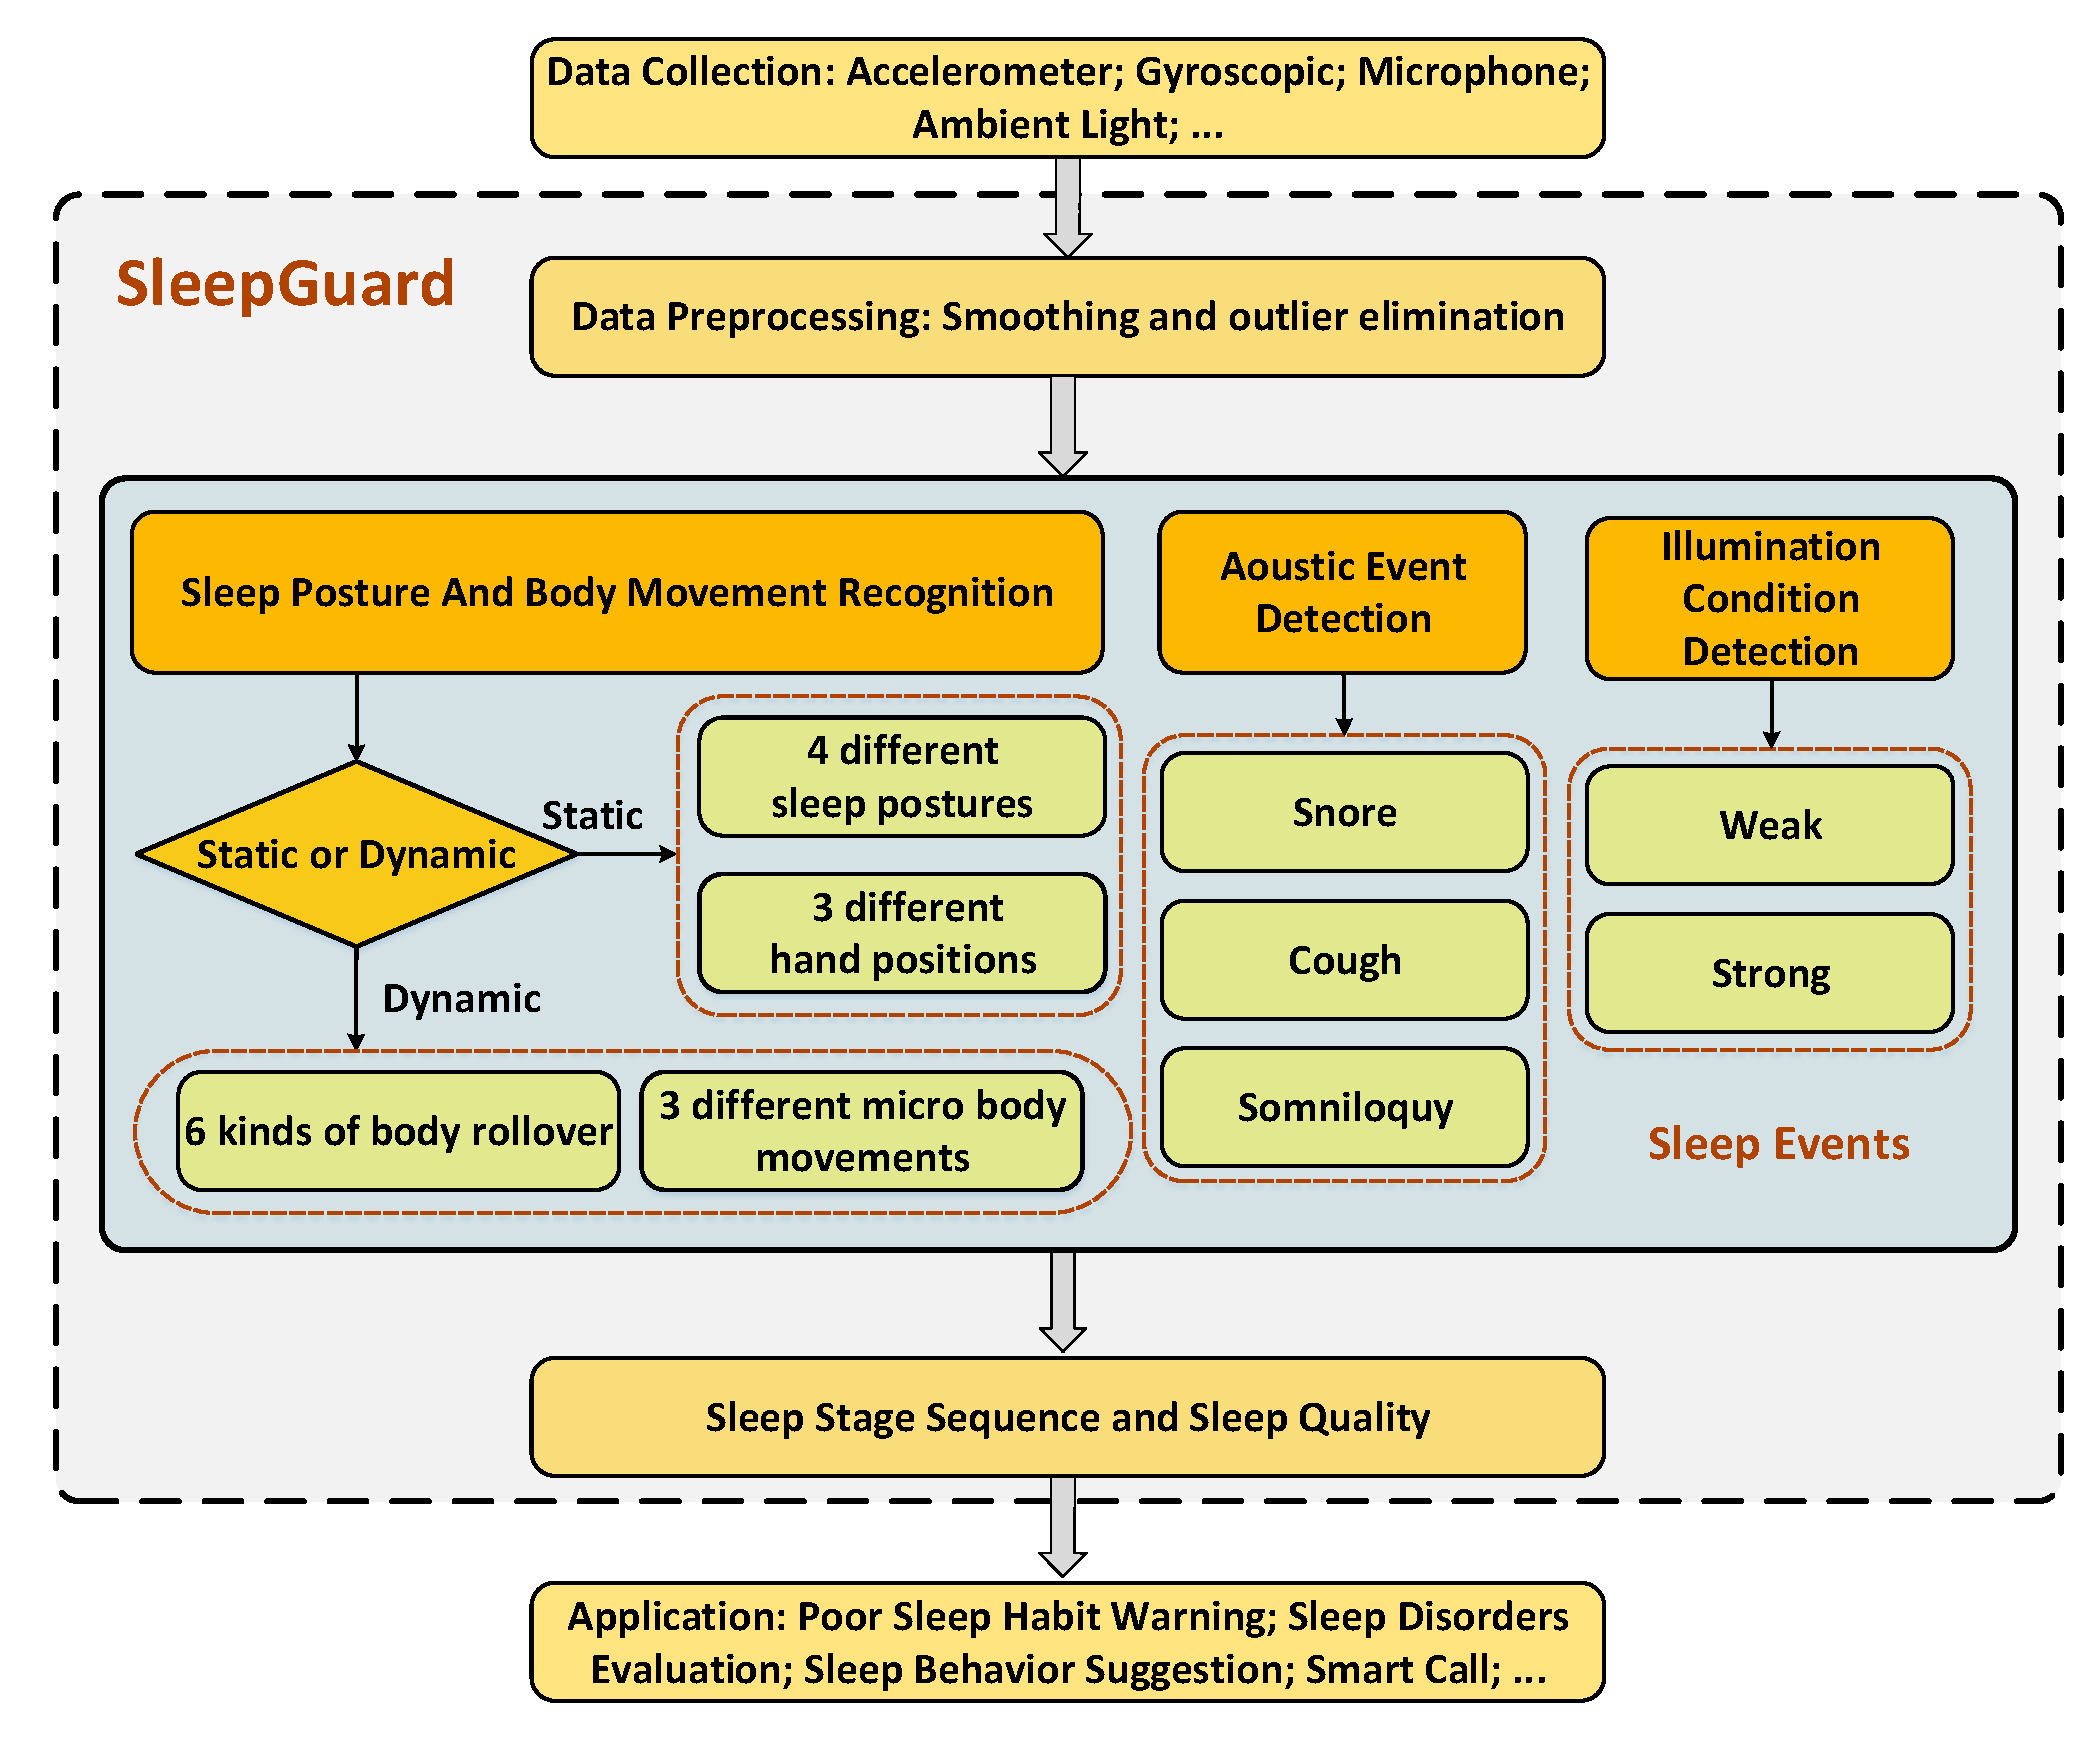
\includegraphics[width=0.97\linewidth]{Figures/SystemFlow.pdf}
  \caption{System overview of {\systemname}.}\label{fig:overview}
\end{figure}


\begin{itemize}[itemsep=1mm,nolistsep]
  \item {\textbf{Data Collection and Preprocessing.}} A variety of sensing data are related to sleep events include i) the accelerometer and the gyroscope about the body movement, ii) the microphone measured acoustic sound, iii) the ambient light sensor about the illumination condition, and iv) the orientation sensor with some auxiliary information. The data is collected every 30 ms on the smartwatch and transferred to the server (such as a smartphone) via Bluetooth. We use data smoothing and outlier elimination to reduce noise in the raw sensor readings.
  \item \textbf{Sleep Event Detection.} A series of novel algorithms are developed to recognize different sleep events. In particular, some key insights are observed about different body postures, body rollovers, hand positions, micro body movements and acoustic events. Note that before identifying those events, {\systemname} first carries out a coarse-grained detection and judges whether the user is lying or not.  After that, we can estimate the user's bedtime. During the user is lying on the bed,  we regard that the user fell asleep if we do not detect a large movement within 20 minutes.
  \item \textbf{{Sleep Pattern Report.}} Sleep Pattern Report. After we obtain the detected sleep events, we integrate them to the clock information, illumination condition, and then use the Hidden Markov Model to infer the sleep stages and evaluate sleep quality. Different from existing apps on the market, {\systemname} provides detailed procedure about the sleep report. The output of our system, for example, sleep postures and the position of user's hand could be used as input to build a broad range of sleeping quality and  heathy applications, such as poor sleep habit warning, the evaluation of insomnia, nightmare and sleep disorders. With the extensive experiments conducted, we conclude that {\systemname} exhibits a relatively high accuracy comparing to state-of-the-art systems.
\end{itemize}


%\subsection{Feature Calculation and Selection}
%Appropriate  features  can  reflect  the  potential  information  underlying the  signals. The  features  used  in {\systemname} are shown in  Table \ref{Tab1}. To detect different sleep events, we use two main features. The first one is the movement related features, that are angle of inclination calculated by acceleration data and the angle of rotation calculated by gyroscopic data. Beyond that, to detect different sound events during sleep, we calculate the energy and zero-crossing rate of the sound signal.
%
%\begin{table}[!thbp]
%\centering
% \caption{Calculated Features}\label{Tab1}
%   \renewcommand\arraystretch{1.7}{\multirowsetup}{\centering}
%        \begin{tabular}{c|c|c}
%        \hline
%        {\bf{Data}}  &   {\bf{Feature}} &   {\bf{Formula}}\\
%         \hline
%        {$acc$} & {Tilt Angle}   & $ A_x =\arccos(\frac {acc_x}{acc}) $ \\
%        \hline
%        {$\omega$} &  {Rotation Angle}  & $ \theta = \int\omega $ \\
%        \hline
%        %\multirow{2} {0.1cm}
%        {Sound}  & Energy   &$ E=\sum\nolimits_{n=-\infty}^{\infty}|x^2(n)|$ \\
%         {$x(n)$}  & Zero-crossing  & $Z$ \\
%          \hline
%\end{tabular}
%\end{table}


\section{SYSTEM DESIGN}\label{Sec:3design}

\textcolor{blue}{\section{SYSTEM OVERVIEW}}
In this section, we present the overview of {\systemname}. It is a system based on smartwatch that can recognize different sleep-related events and report the details. Three main modules are illustrated in Fig. \ref{fig:overview}.

\begin{figure}[!thbp]
\centering
%\setlength{\belowcaptionskip}{-9pt}
      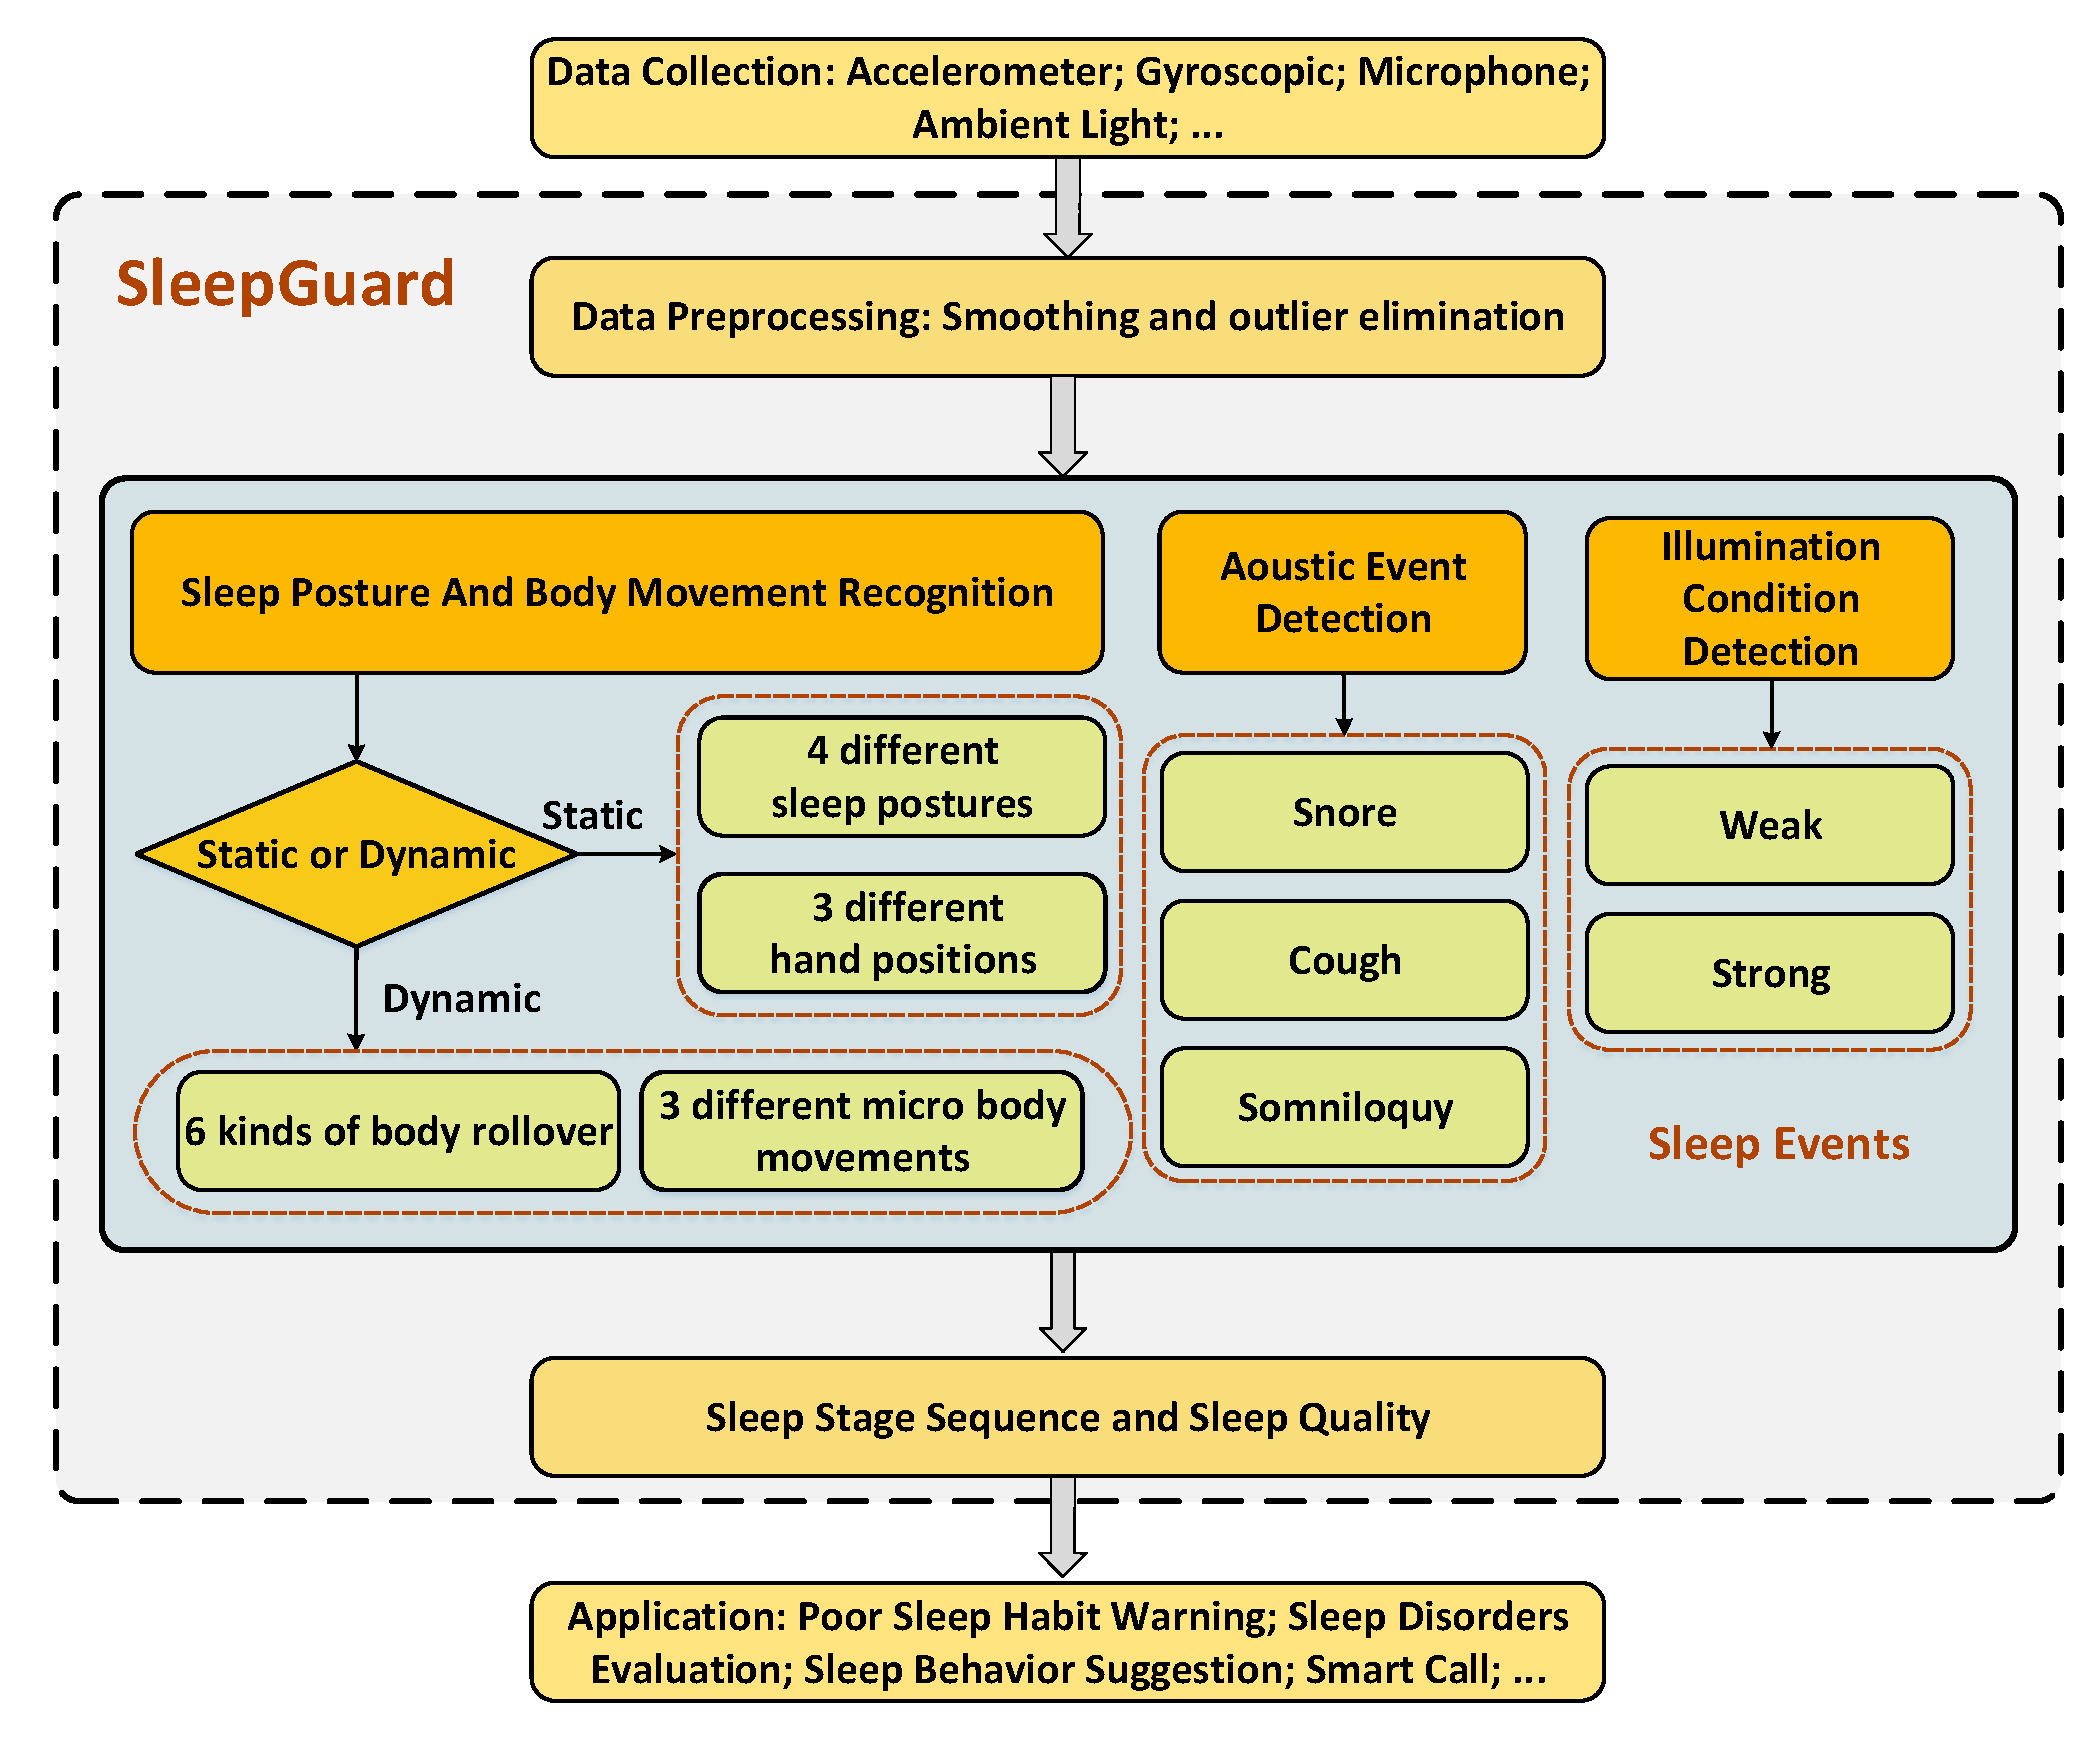
\includegraphics[width=0.97\linewidth]{Figures/SystemFlow.pdf}
  \caption{System overview of {\systemname}.}\label{fig:overview}
\end{figure}


\begin{itemize}[itemsep=1mm,nolistsep]
  \item {\textbf{Data Collection and Preprocessing.}} A variety of sensing data are related to sleep events include i) the accelerometer and the gyroscope about the body movement, ii) the microphone measured acoustic sound, iii) the ambient light sensor about the illumination condition, and iv) the orientation sensor with some auxiliary information. The data is collected every 30 ms on the smartwatch and transferred to the server (such as a smartphone) via Bluetooth. We use data smoothing and outlier elimination to reduce noise in the raw sensor readings.
  \item \textbf{Sleep Event Detection.} A series of novel algorithms are developed to recognize different sleep events. In particular, some key insights are observed about different body postures, body rollovers, hand positions, micro body movements and acoustic events. Note that before identifying those events, {\systemname} first carries out a coarse-grained detection and judges whether the user is lying or not.  After that, we can estimate the user's bedtime. During the user is lying on the bed,  we regard that the user fell asleep if we do not detect a large movement within 20 minutes.
  \item \textbf{{Sleep Pattern Report.}} Sleep Pattern Report. After we obtain the detected sleep events, we integrate them to the clock information, illumination condition, and then use the Hidden Markov Model to infer the sleep stages and evaluate sleep quality. Different from existing apps on the market, {\systemname} provides detailed procedure about the sleep report. The output of our system, for example, sleep postures and the position of user's hand could be used as input to build a broad range of sleeping quality and  heathy applications, such as poor sleep habit warning, the evaluation of insomnia, nightmare and sleep disorders. With the extensive experiments conducted, we conclude that {\systemname} exhibits a relatively high accuracy comparing to state-of-the-art systems.
\end{itemize}


%\subsection{Feature Calculation and Selection}
%Appropriate  features  can  reflect  the  potential  information  underlying the  signals. The  features  used  in {\systemname} are shown in  Table \ref{Tab1}. To detect different sleep events, we use two main features. The first one is the movement related features, that are angle of inclination calculated by acceleration data and the angle of rotation calculated by gyroscopic data. Beyond that, to detect different sound events during sleep, we calculate the energy and zero-crossing rate of the sound signal.
%
%\begin{table}[!thbp]
%\centering
% \caption{Calculated Features}\label{Tab1}
%   \renewcommand\arraystretch{1.7}{\multirowsetup}{\centering}
%        \begin{tabular}{c|c|c}
%        \hline
%        {\bf{Data}}  &   {\bf{Feature}} &   {\bf{Formula}}\\
%         \hline
%        {$acc$} & {Tilt Angle}   & $ A_x =\arccos(\frac {acc_x}{acc}) $ \\
%        \hline
%        {$\omega$} &  {Rotation Angle}  & $ \theta = \int\omega $ \\
%        \hline
%        %\multirow{2} {0.1cm}
%        {Sound}  & Energy   &$ E=\sum\nolimits_{n=-\infty}^{\infty}|x^2(n)|$ \\
%         {$x(n)$}  & Zero-crossing  & $Z$ \\
%          \hline
%\end{tabular}
%\end{table}



\begin{figure}[!thbp]
\centering
%\setlength{\belowcaptionskip}{-9pt}
      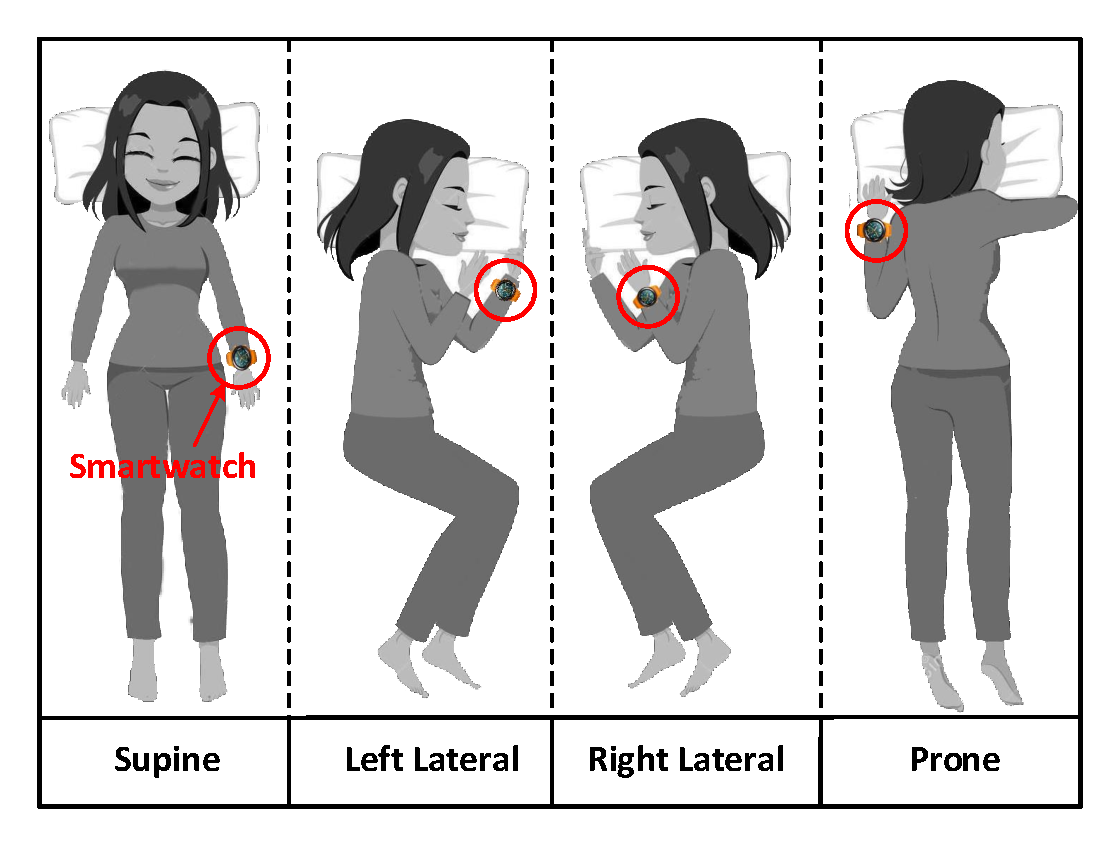
\includegraphics[width=0.87\linewidth]{Figures/BodyPosture.pdf}
  \caption{Four sleep body postures.}\label{fig:BodyPosture}
\end{figure}

\begin{figure}[!t]
  \centering
  \subfigure[Supine]{
    \label{fig:Supine}
    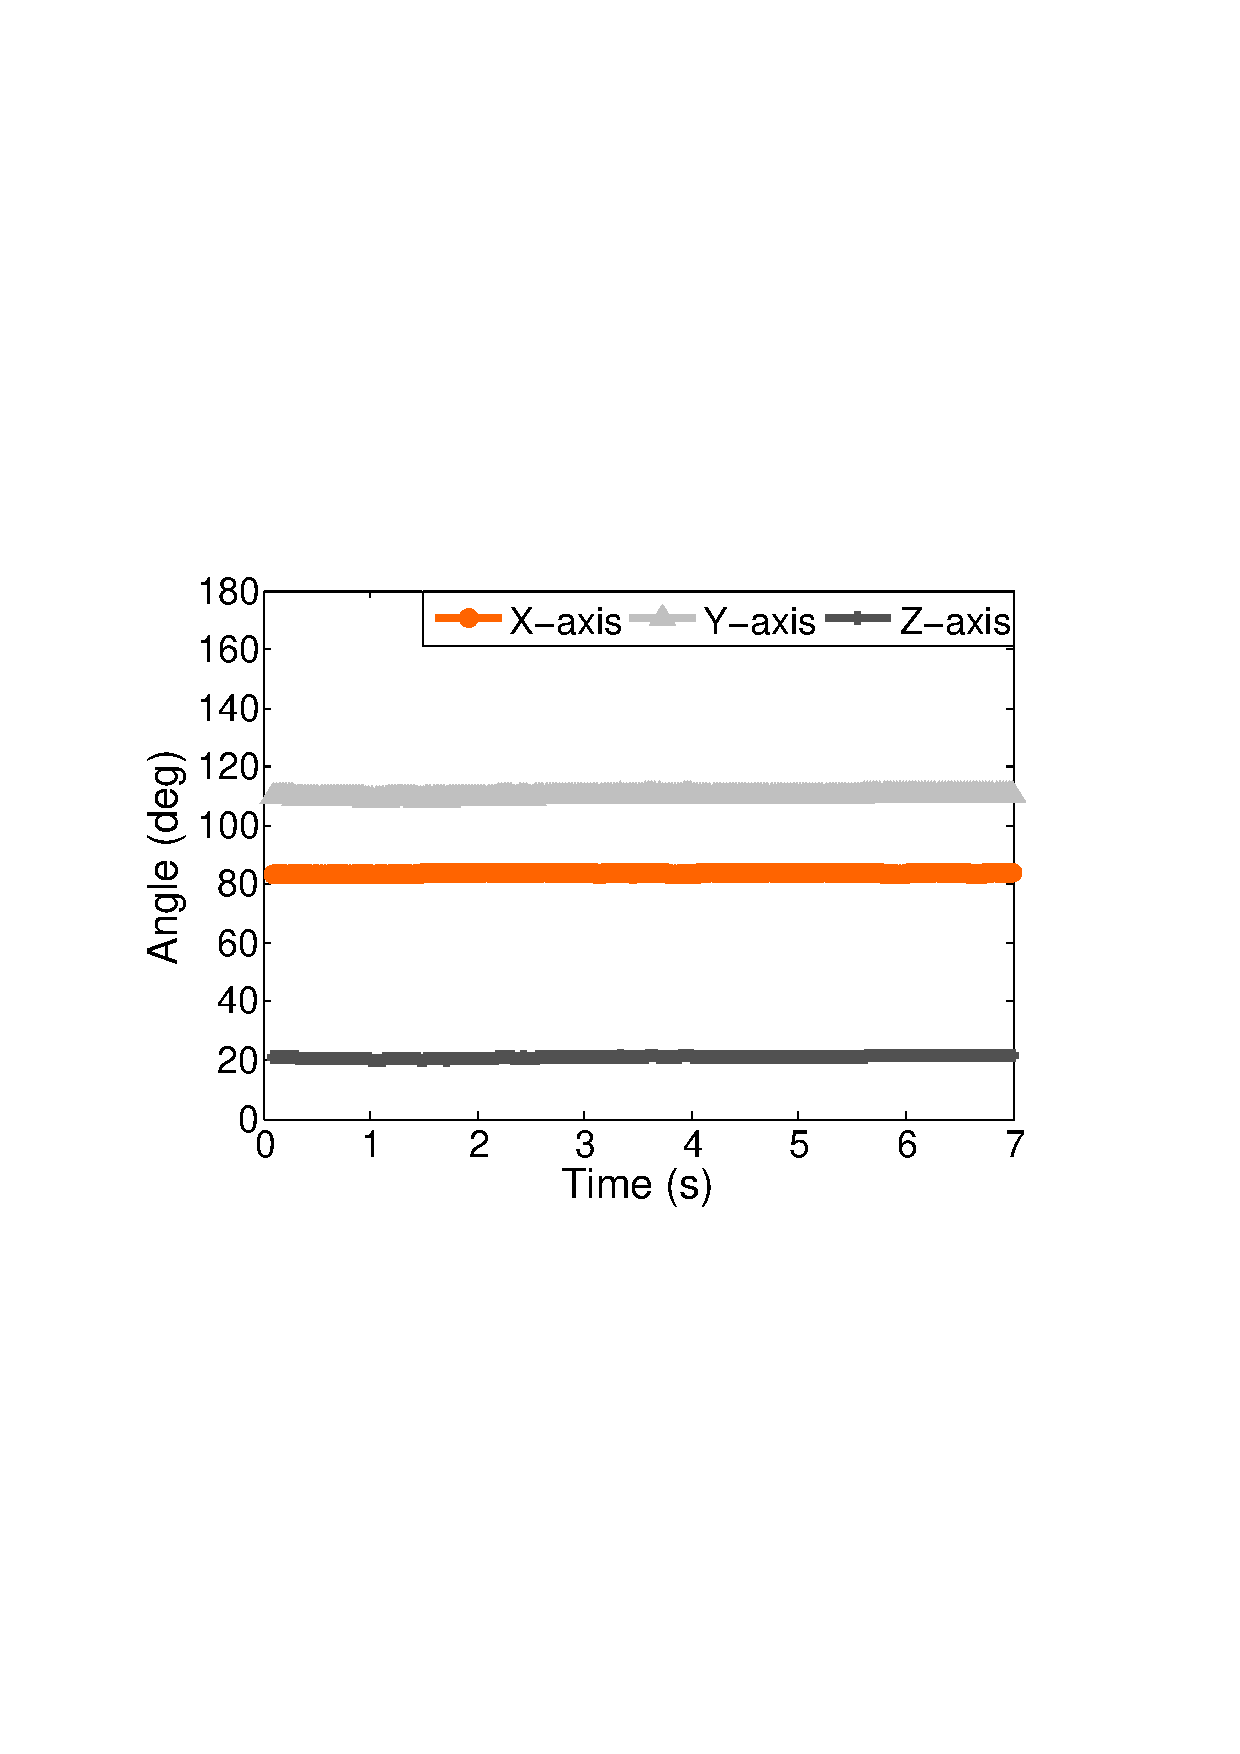
\includegraphics[width=0.47\linewidth]{Figures/Supine.pdf}}
  \hfill
  \subfigure[Left Lateral]{
    \label{fig:LeftLateral}
    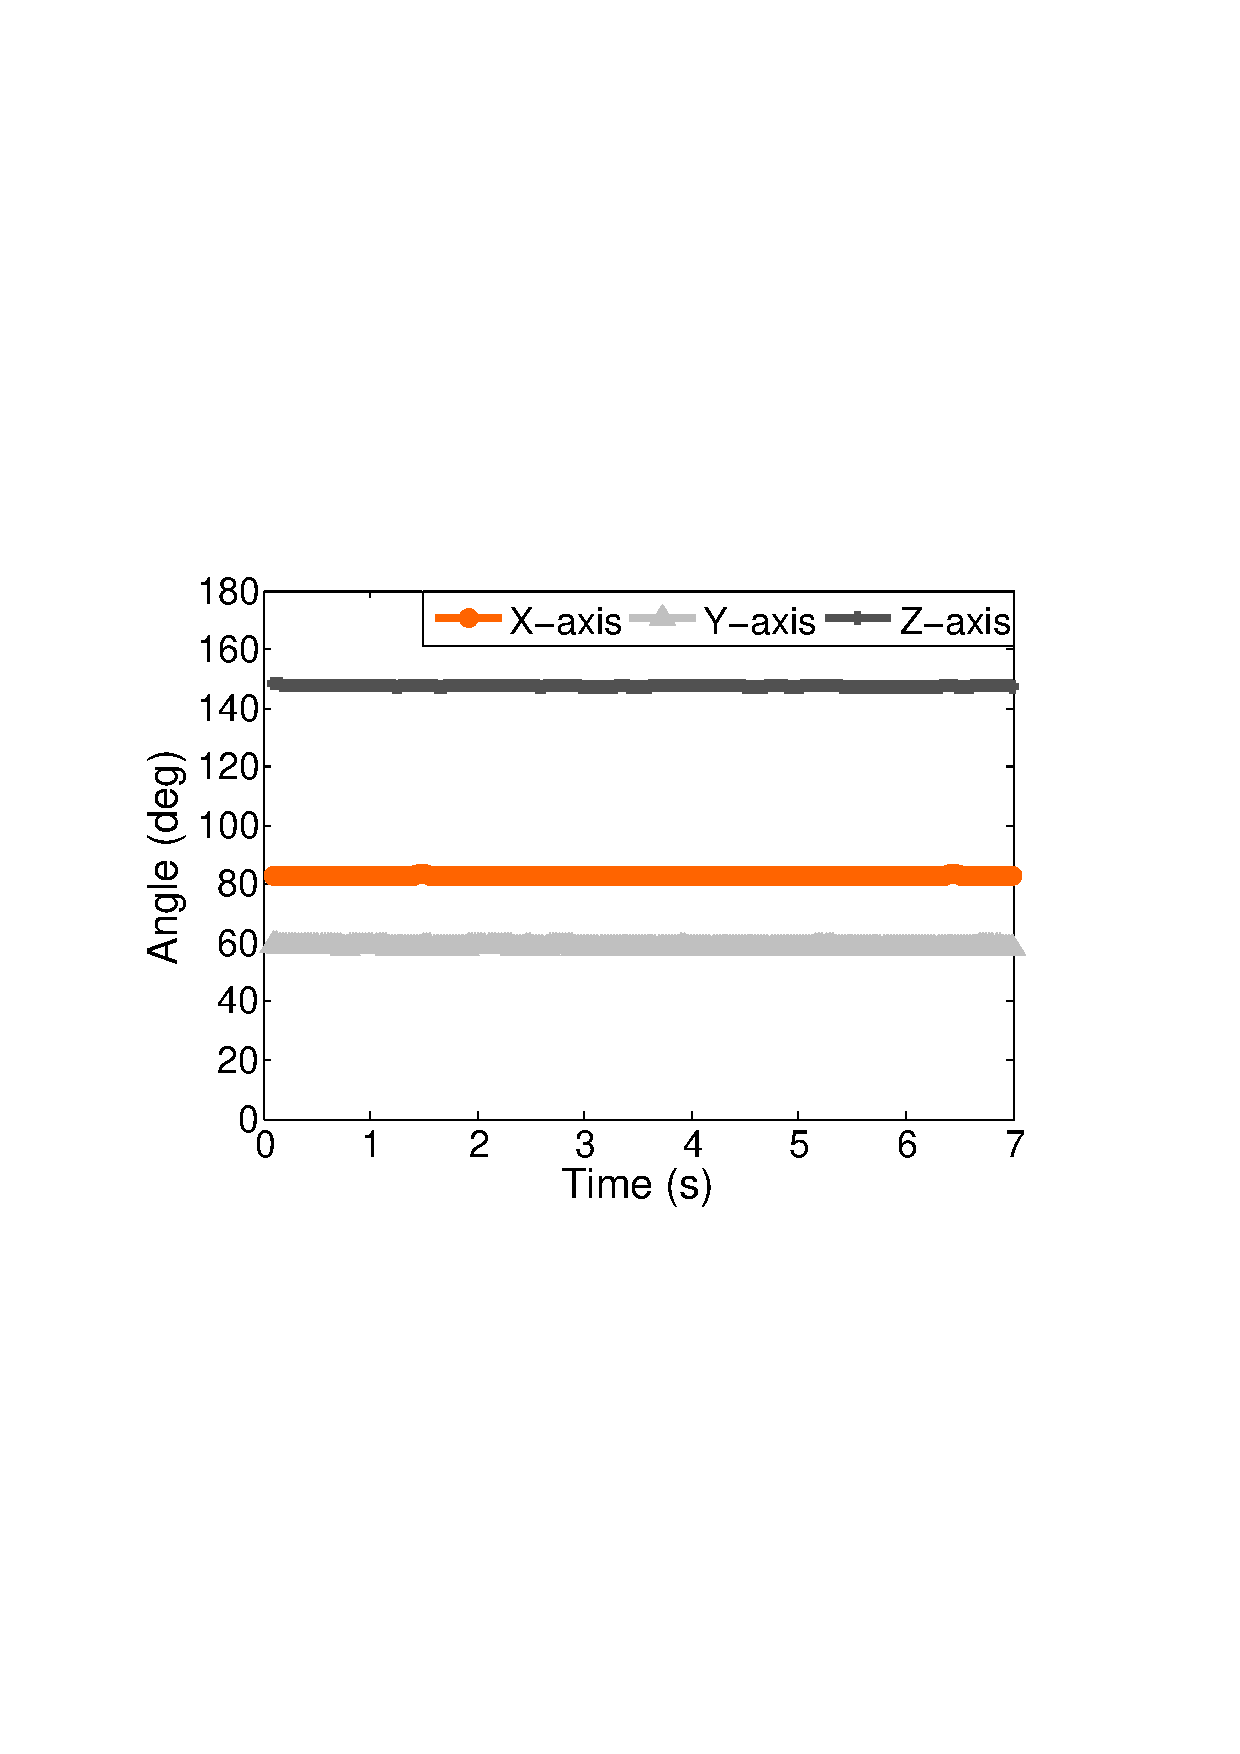
\includegraphics[width=0.47\linewidth]{Figures/LeftLateral.pdf}}
   \subfigure[Right Lateral]{
    \label{fig:RightLateral}
    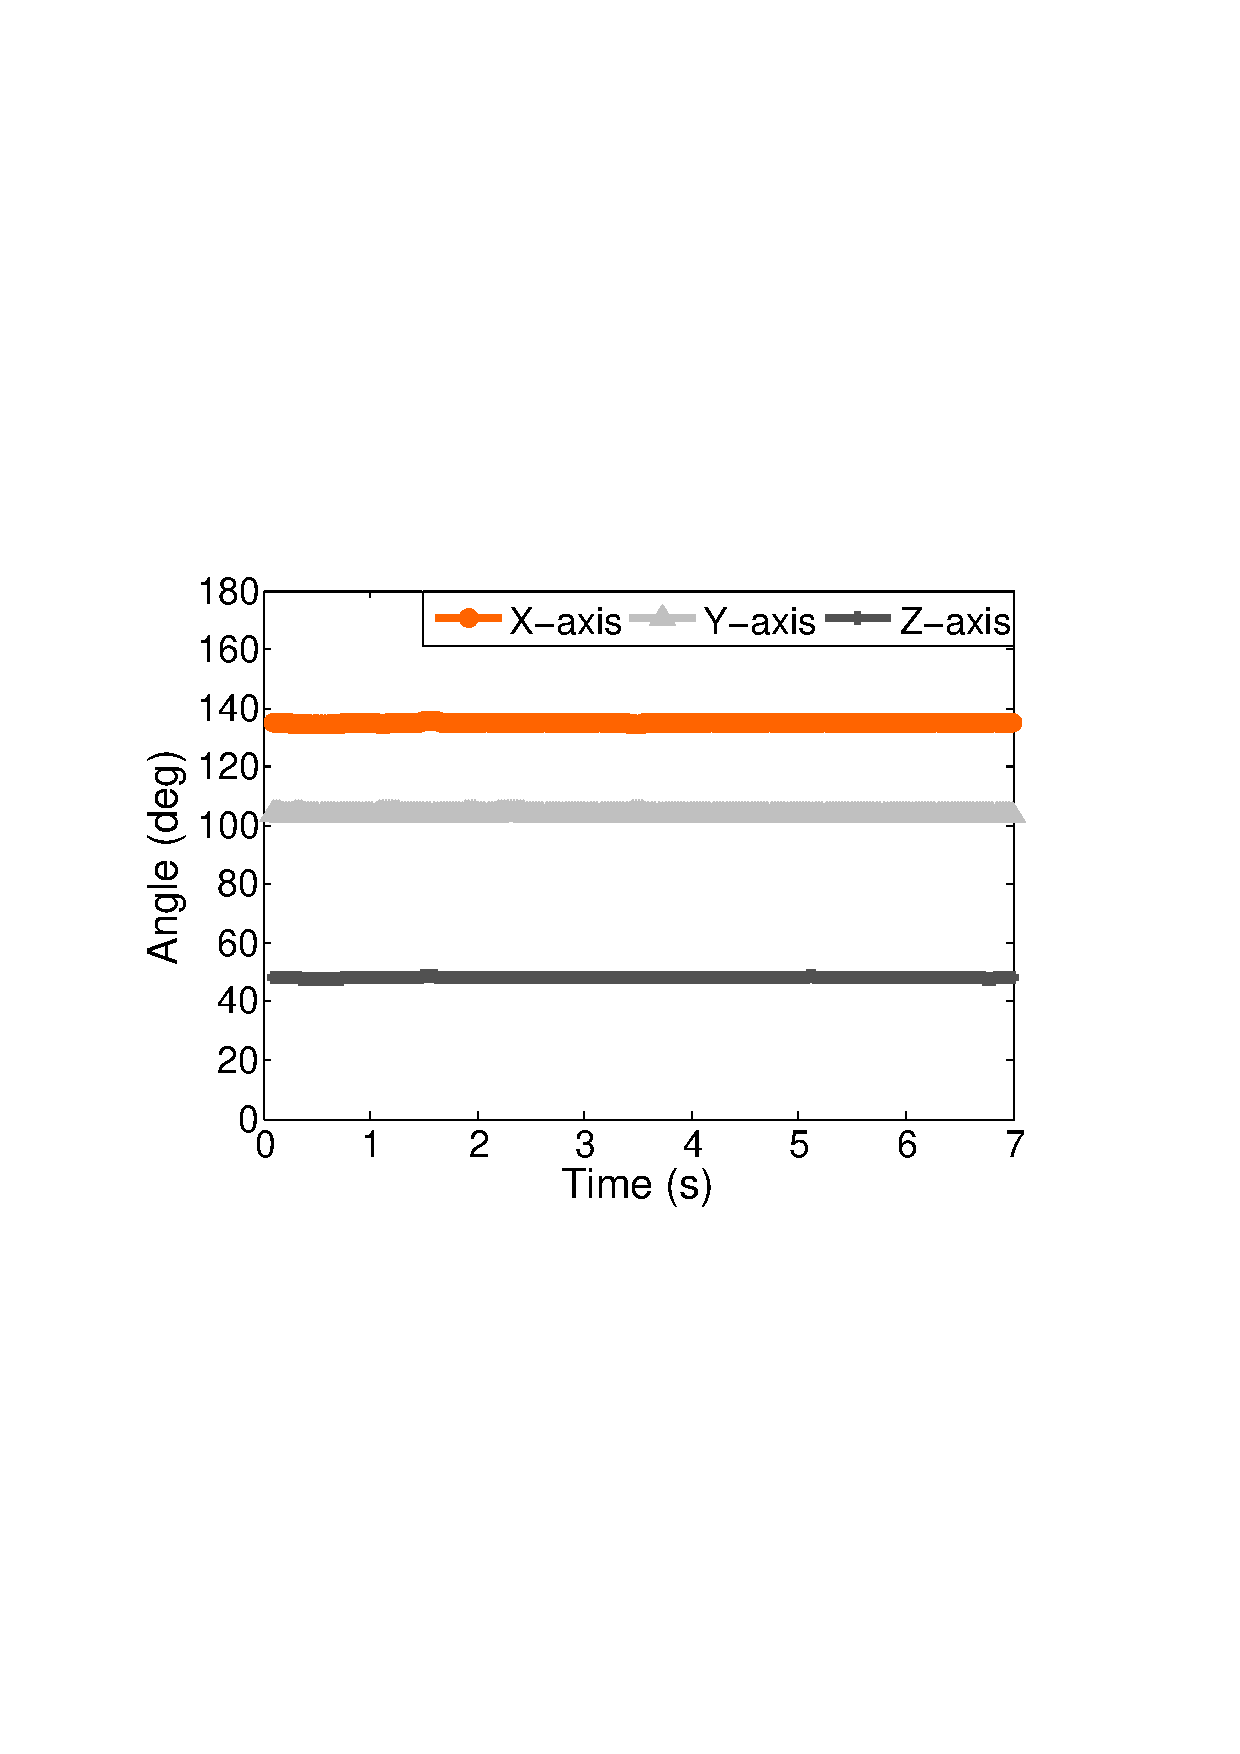
\includegraphics[width=0.47\linewidth]{Figures/RightLateral.pdf}}
  %\hspace{1in}
  \hfill
  \subfigure[Prone]{
    \label{fig:Prone}
    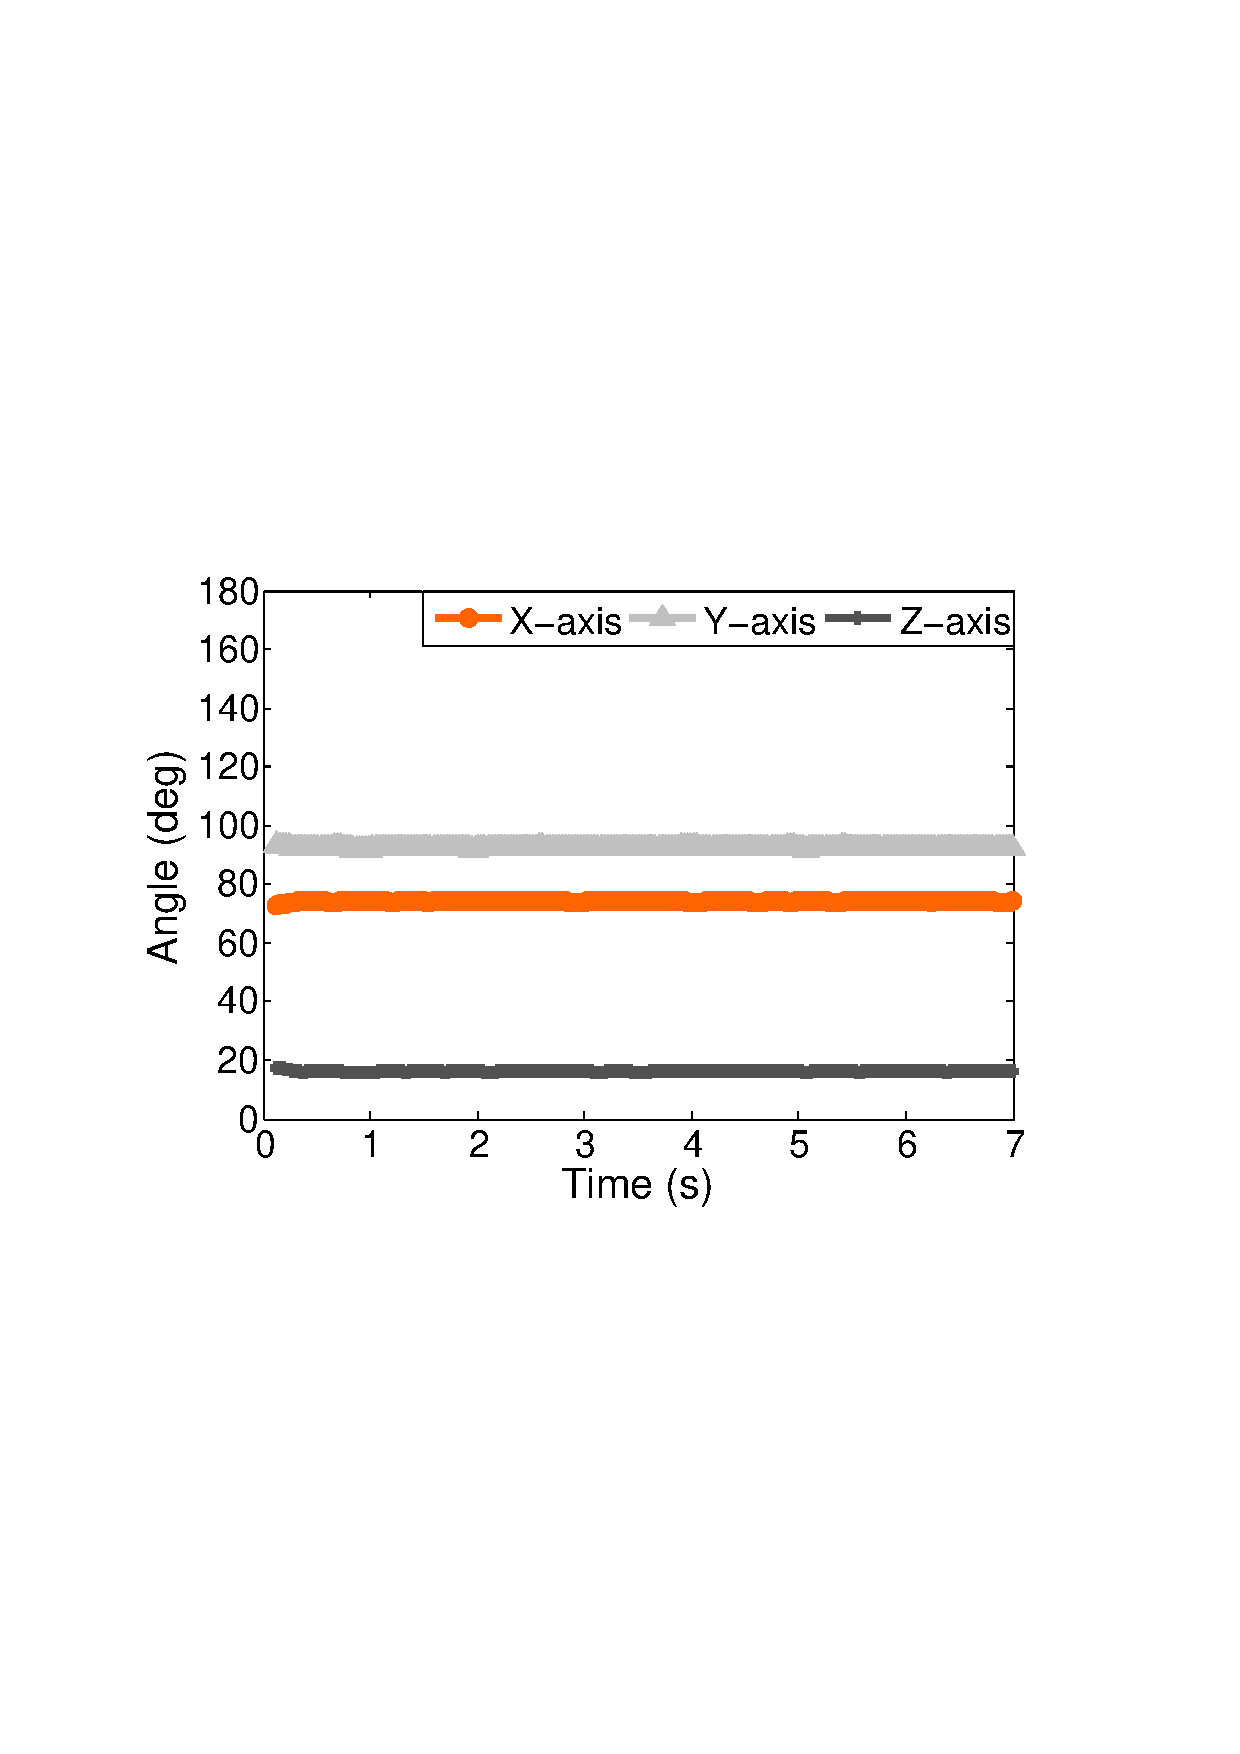
\includegraphics[width=0.47\linewidth]{Figures/Prone.pdf}}
  \caption{The tilt angle characteristics of four body postures.}
  \label{fig:posture}
\end{figure}

\subsection{Sleep Posture and Movement}
{\systemname} can monitor the user's sleep posture and habits, which is an indispensable factor of determining sleep quality and is heavily used in performing medical diagnoses \cite{oksenberg1998effect}. We present the detection details about the body posture and movement events. In {\systemname}, there are 4 different sleep postures, 3 different hand positions, 6 kinds of body rollover and 3 different micro body movements considered.  These events comprehensively and highly relates to the sleep stages and quality.

\subsubsection{Body posture detection}
According to research, dreaming and sleep quality are associated with underlying brain functions and may be affected by body posture \cite{posture2004}. And for different people, they should have his own fit sleeping posture, taking into account his own physical factors \cite{posture2016,posture2017}. For example, people with ailments such as heart disease or high blood pressure are unfit for prone position. People can consciously avoid or take some kind of sleep posture, which will have very good benefits for sleep quality and health \cite{posture2015}. So an effective posture detection and timely posture change can improve the sleep quality and avoid the harm for health. We concentrate on four common body postures, that are supine, left lateral, right lateral and prone. According to our survey, most people's arms have some usual and  fixed positions in these four different sleeping positions, namely the arm's position is related to the body posture, which is similar to the idea of the sleep posture detection in \cite{sleepmonitor}. In {\systemname}, we consider the following situations. when user sleep in supine, we consider that user's hand put on the left sides of the body, on the abdomen, on the chest or on the head; when user sleep on left, we consider that user's hand put close to the pillow; When user sleep on right, the hand on the chest, on the waist or close to the pillow are considered by our system; And the hand on the side of the head or above the head, we consider, when user sleep in the prone posture. In the future work, we will consider more of the arm's position. Fig. \ref{fig:BodyPosture} shows that one of a position of arm in four different sleep postures.

We can choose the three-axis tilt angle calculated from the acceleration data as the feature \cite{sleepmonitor}. And then we use a supervised learning method to create a sleep posture profile. Specifically, we collect training data to create a mapping (i.e., angle mapping) between the angles and the arm under different positions. In order to extract the window-based tilt angle features, we average all the calculated angles in a window. Fig. \ref{fig:posture} shows the characteristics of four sleep postures with, it indicates that the tilt angles of three axes have obvious differences.The sleep postures thus can be inferred based on the positions of the smartwatch and the created angle mapping. However, we found that the supine features when the hand on the left sides of the body are similar with the prone features when the hand on the side of the head (Fig. \ref{fig:Supine} and \ref{fig:Prone}), thus the classification accuracy will be affected.

In order to improve the detection accuracy between the supine posture and prone posture, we go further to introduce the orientation sensory data as an auxiliary feature. This is based on the observation that the hand directions in the supine and prone positions are different. When the result of the previous step is prone or supine, we combine the tilt angle with three axes data obtained from the direction sensor as a new feature, and classify these postures more accurately based on the template distance matching. The posture will be detected as the one in the template which has a minimum Euclidean distance to it. Noted that when we use the direction sensor, we must limit the pillow orientation remaining unchanged (in the experiment our pillow is placed on the north). In fact, this assumption can be easily satisfied since most people usually have fixed sleep directions.


\subsubsection{Hand position recognition}
The hand position during sleep discloses some potential health problems and the improper hand position will bring bad results \cite{position2014}. For instance, the hand position on the abdomen may indicate its uncomfortable state, while the person is usually not aware of that cases; when the hand is put on the chest, the person is more likely to have a nightmare because of the long-term oppression on the heart; And when the hand is put on the head, it can put excess pressure on the nerves in your shoulders, shoulder and arm pain is quite common, as blood flow is restricted in this position. This can lead to eventual nerve damage, with symptoms including a tingling sensation and numbness \cite{position2014}. {\systemname} can recognize three hand positions, that are on the abdomen, chest or head when the user is in the supine posture, as shown in Fig. \ref{fig:HandPosition}. Note that because in other body postures, the hand is put on the bed at most time, thus we do not consider different hand positions when the body are in other postures.

\begin{figure}[!t]
\centering
      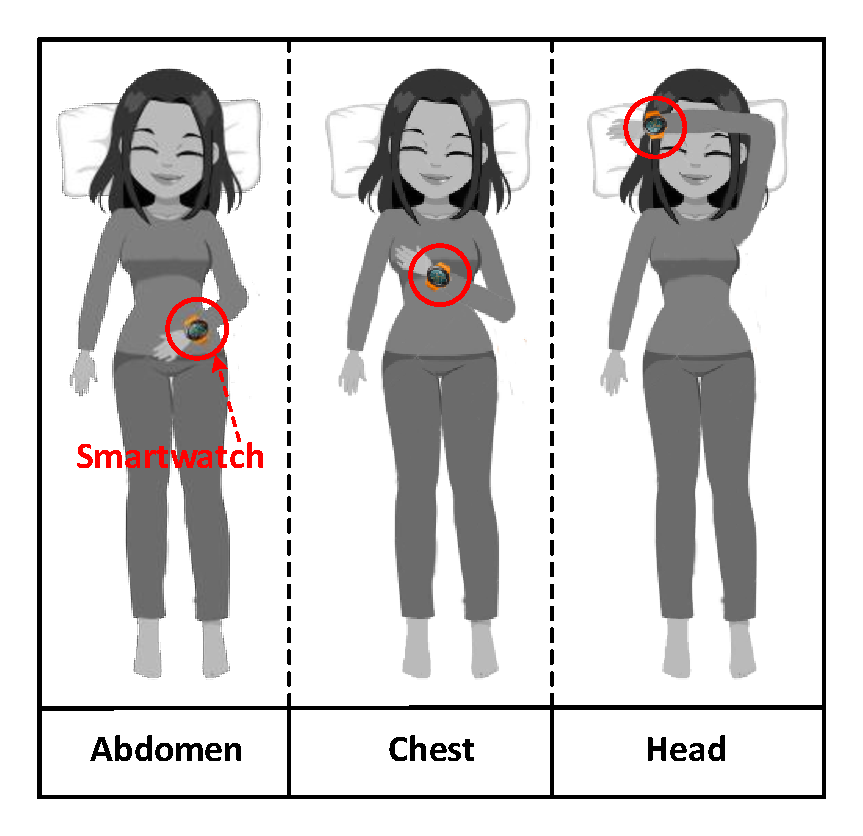
\includegraphics[width=0.7\linewidth,height=4.8cm]{Figures/HandPosition.pdf}
  \caption{Three hand positions.}\label{fig:HandPosition}
\end{figure}


In fact, when people are sleeping in the supine posture, the hands may be on both sides of the body, on the abdomen, chest or head. To identify the hand position accurately, we present a new algorithm based on our key observation. We have observed that before the hand put on the body initially, it usually experiences a movement from the body side to the end position, and after that the hand always experiences a movement from one position to the other. Thus we can further integrate the hand movement trajectory to determine the hand position at current time. In {\systemname}, We consider nine kinds of the trajectories of hand, from the side of the body to the abdomen, to the chest, to the head; from the chest to the abdomen, to the head; from the abdomen to the chest, to the head; from the head to the abdomen, to the chest. Fig. \ref{Bodyhand} shows the rotation angle changes when the hand is moving from the body side to different positions on the body. We use the three-axis rotation angle calculated by the gyroscope as a feature to establish a sample library, and use the template distance matching classifier to identify the final position of the hand.


According to the trajectory of hand movement can roughly determine the shot in the head, or in the part close to the chest, or in the part near the abdomen. However, depending on the trajectory, we can not be sure that the hand is exactly in the chest or abdomen. This is because when the hand move to the shoulder or hip and some other areas close to the chest or abdomen, we can know that the trajectories of the hand are very similar, so we need to go further to determine the hand on the chest or abdomen. Obviously, when the hand is put on the abdomen or chest, we can see that the acceleration signals exhibit a distinctly periodic fluctuation, as shown in Fig. \ref{Bodyhand}. This is due to the movement of the abdomen and chest caused by breathing.Therefore, we can use the occurrence of respiratory events to determine if the hand is indeed on the body (abdomen or chest). Specifically, we calculate the power spectral density (PSD) of the acceleration signal, where the highest peak frequency is the signal's frequency. From Fig. \ref{fig:PSD}, we can see that there is a large peak located at around 0.25 Hz, which corresponds the respiratory frequency. So if the signal's frequency falls within the reasonable breathing frequency range, which is around 20 times per minute (0.3 Hz), it indicates the occurrence of respiration events, that is, the hand is put on the chest or abdomen.

In addition, we found that the extent of body movements can be used to judge the amplitude of respiration. What's more, we know that when people sleep in the REM stage, they respiratory amplitude smaller than the respiratory amplitude sleep in the NREM stage \cite{respiratory1982}, so we can roughly determine the user's current sleep stage based on the respiratory amplitude. Of course, respiratory amplitude is only an indicator of the division of the sleep stage, we can not regard it as a basis for final judgment, only for reference here and it can help later detection of the sleep stage. Under normal circumstances, the chest movement amplitude is smaller than abdominal movement amplitude. However, in different sleep stages, the respiration amplitudes are different \cite{respiratory}. It is likely that there is a situation: the chest movement amplitude in the NREM sleep stage is close to the abdominal movement amplitude in the REM sleep stage. As a result, the threshold based method cannot work. At this time, we need to combine it with the position of the hand we detected with the trajectory before. Through the above steps, we have been able to determine whether the hands are on the chest or abdomen, and then we can go further to determine the extent of breathing according to the degree of body ups and downs, and we can roughly infer the sleep stage. Now we take the case of hands on the abdomen as an example.

\begin{figure}[!t]
  \centering
   %\begin{minipage}[t]{0.325\linewidth}
  \subfigure[]{\label{BodytoAbdomen}
   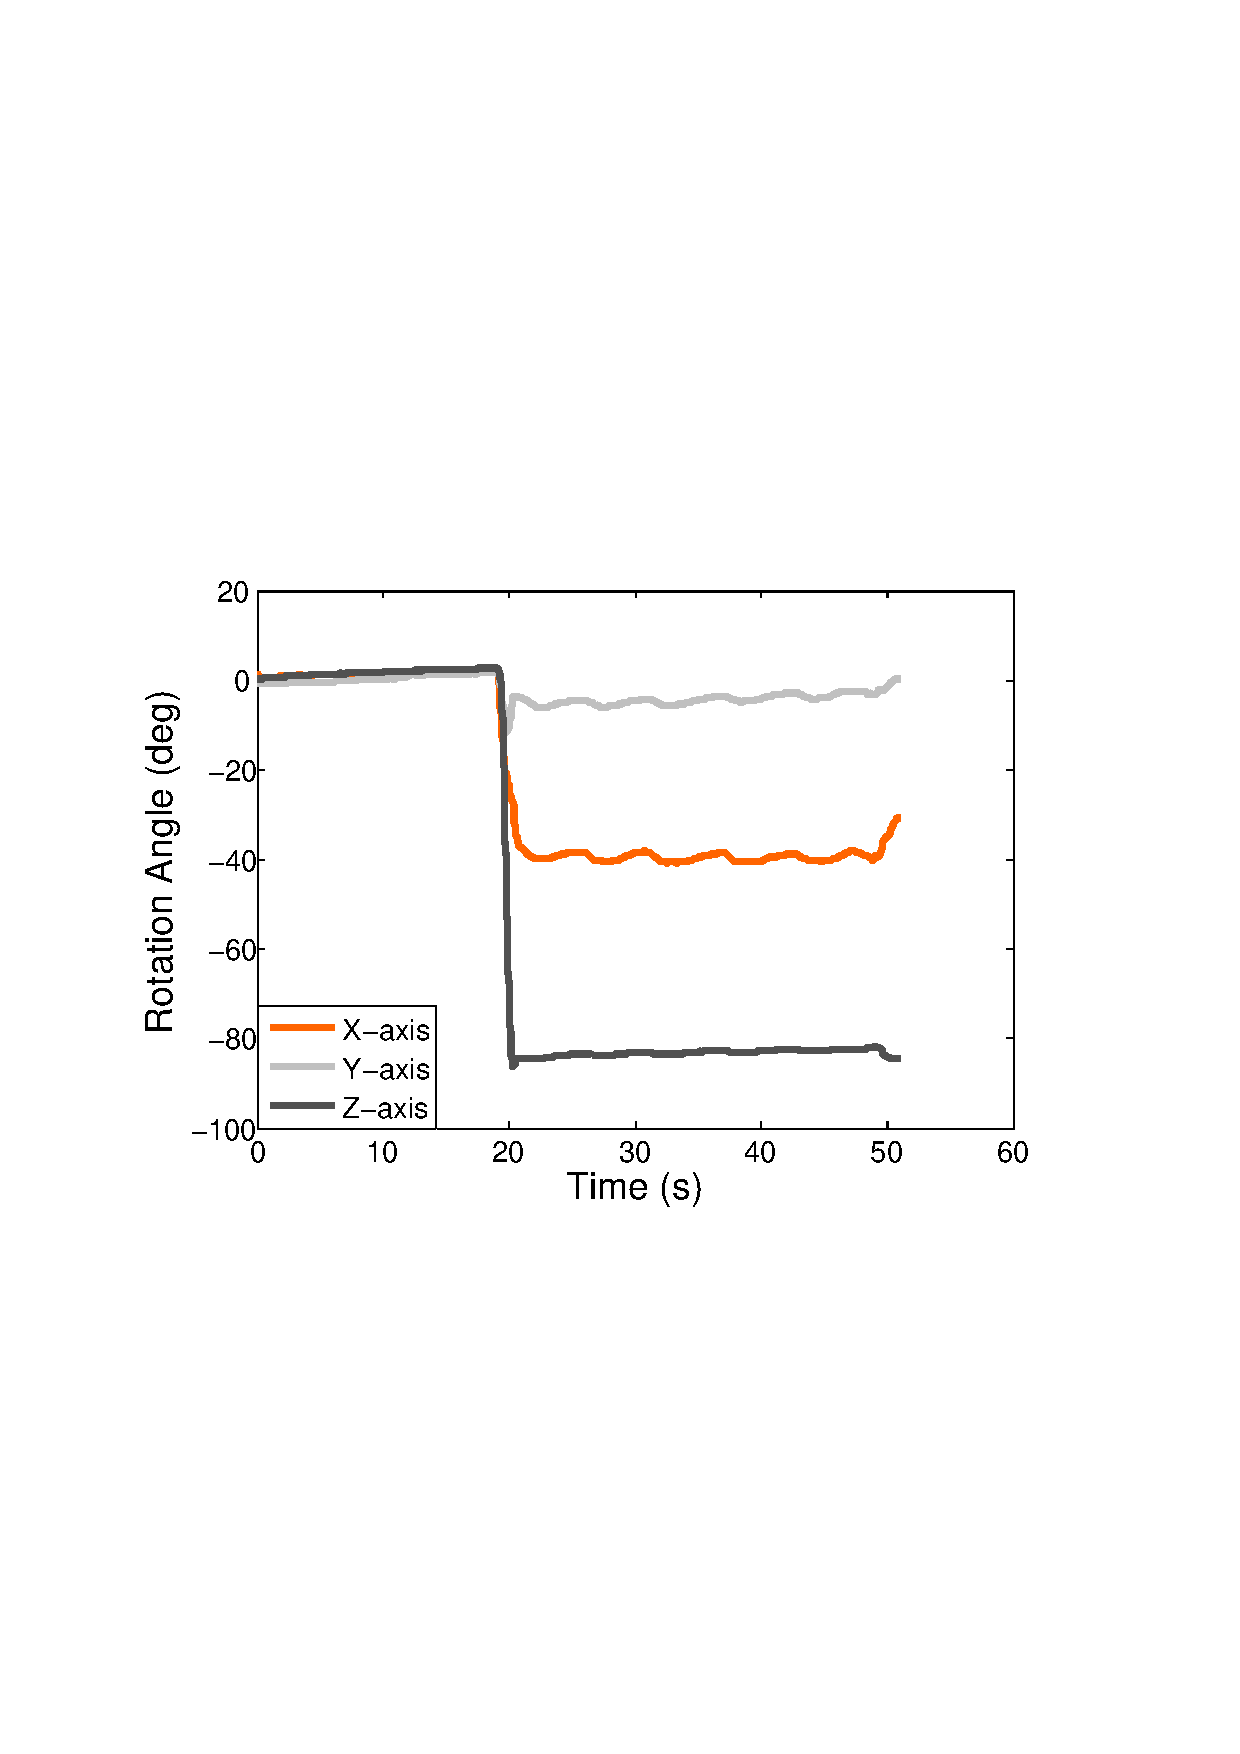
\includegraphics[width=2.7cm,height=2cm]{Figures/BodytoAbdomen.pdf}}
%  \hfill
   \subfigure[]{\label{BodytoChest}
   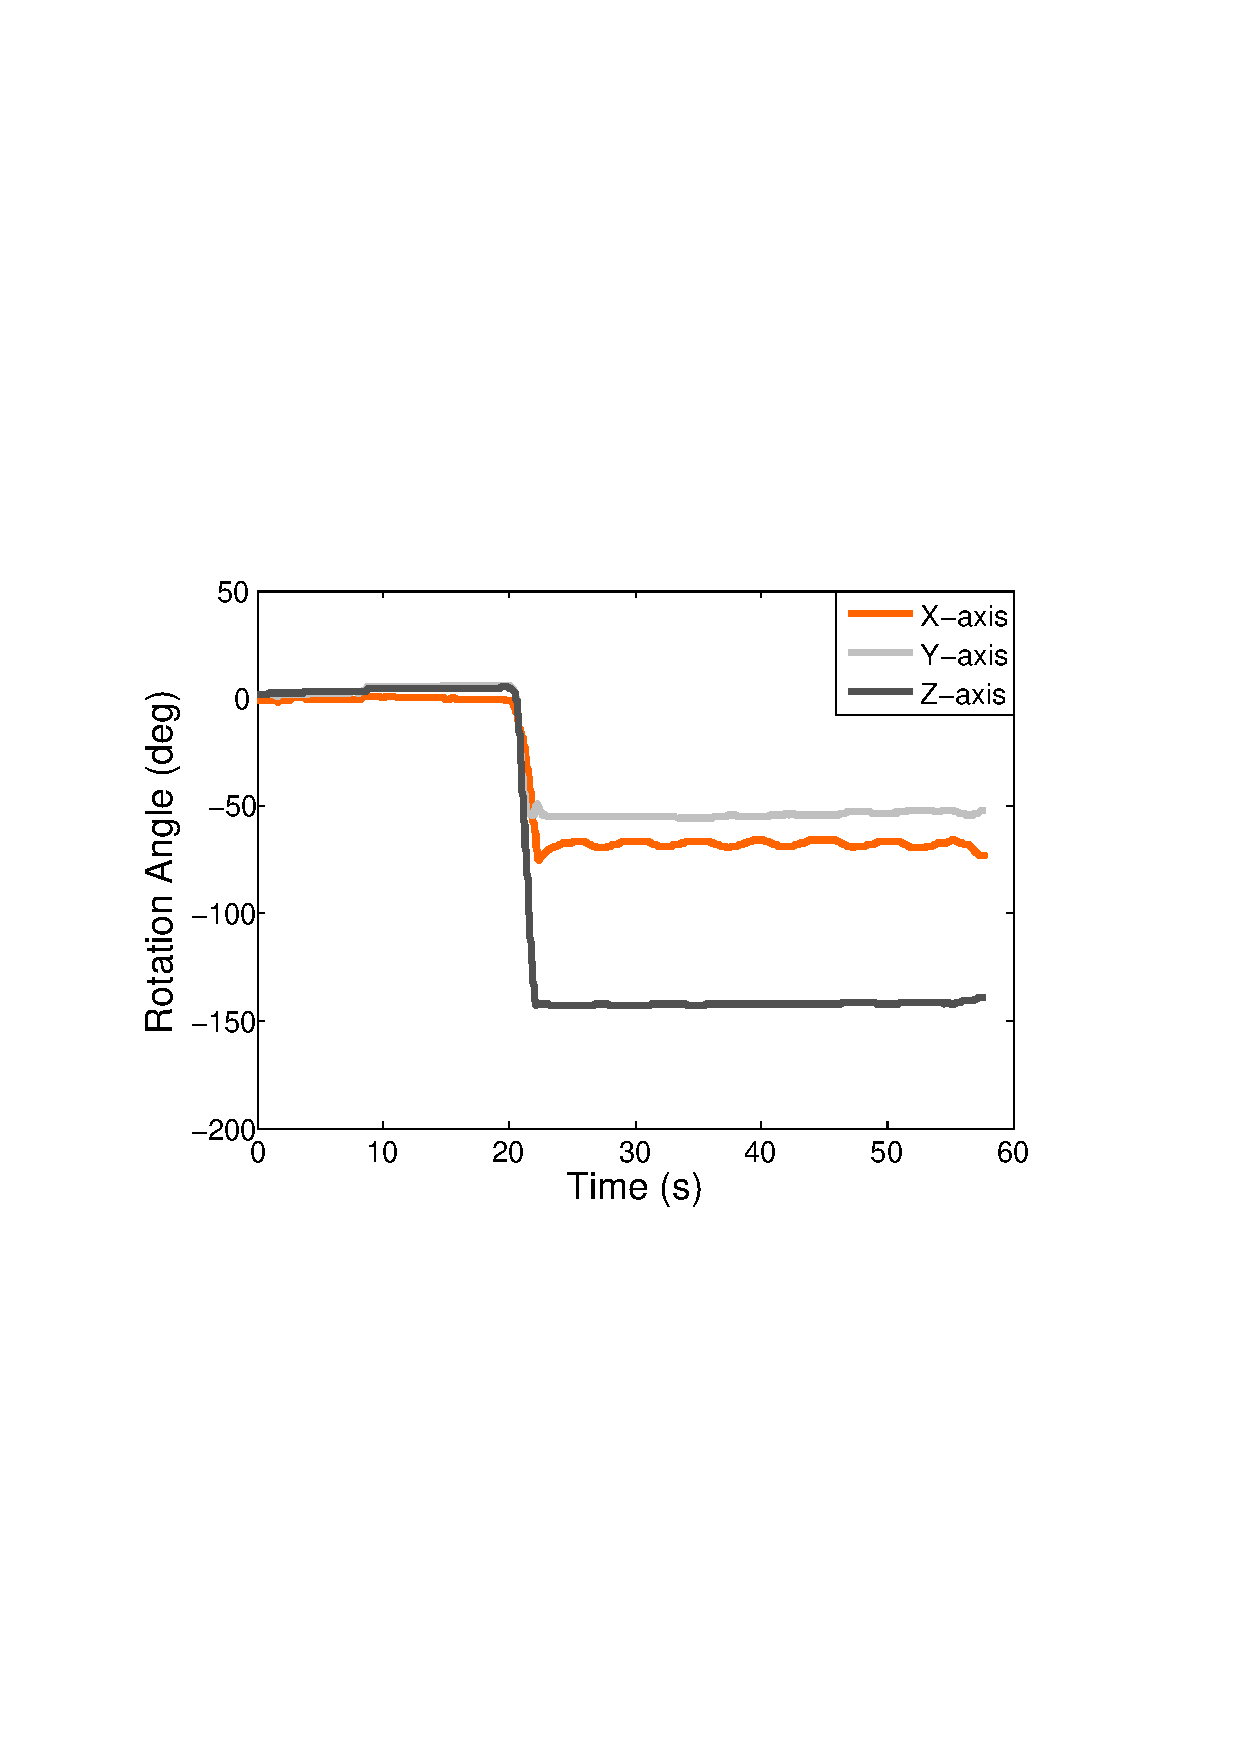
\includegraphics[width=2.7cm,height=2cm]{Figures/BodytoChest.pdf}}
%  \hfill
  \subfigure[]{\label{BodytoHead}
   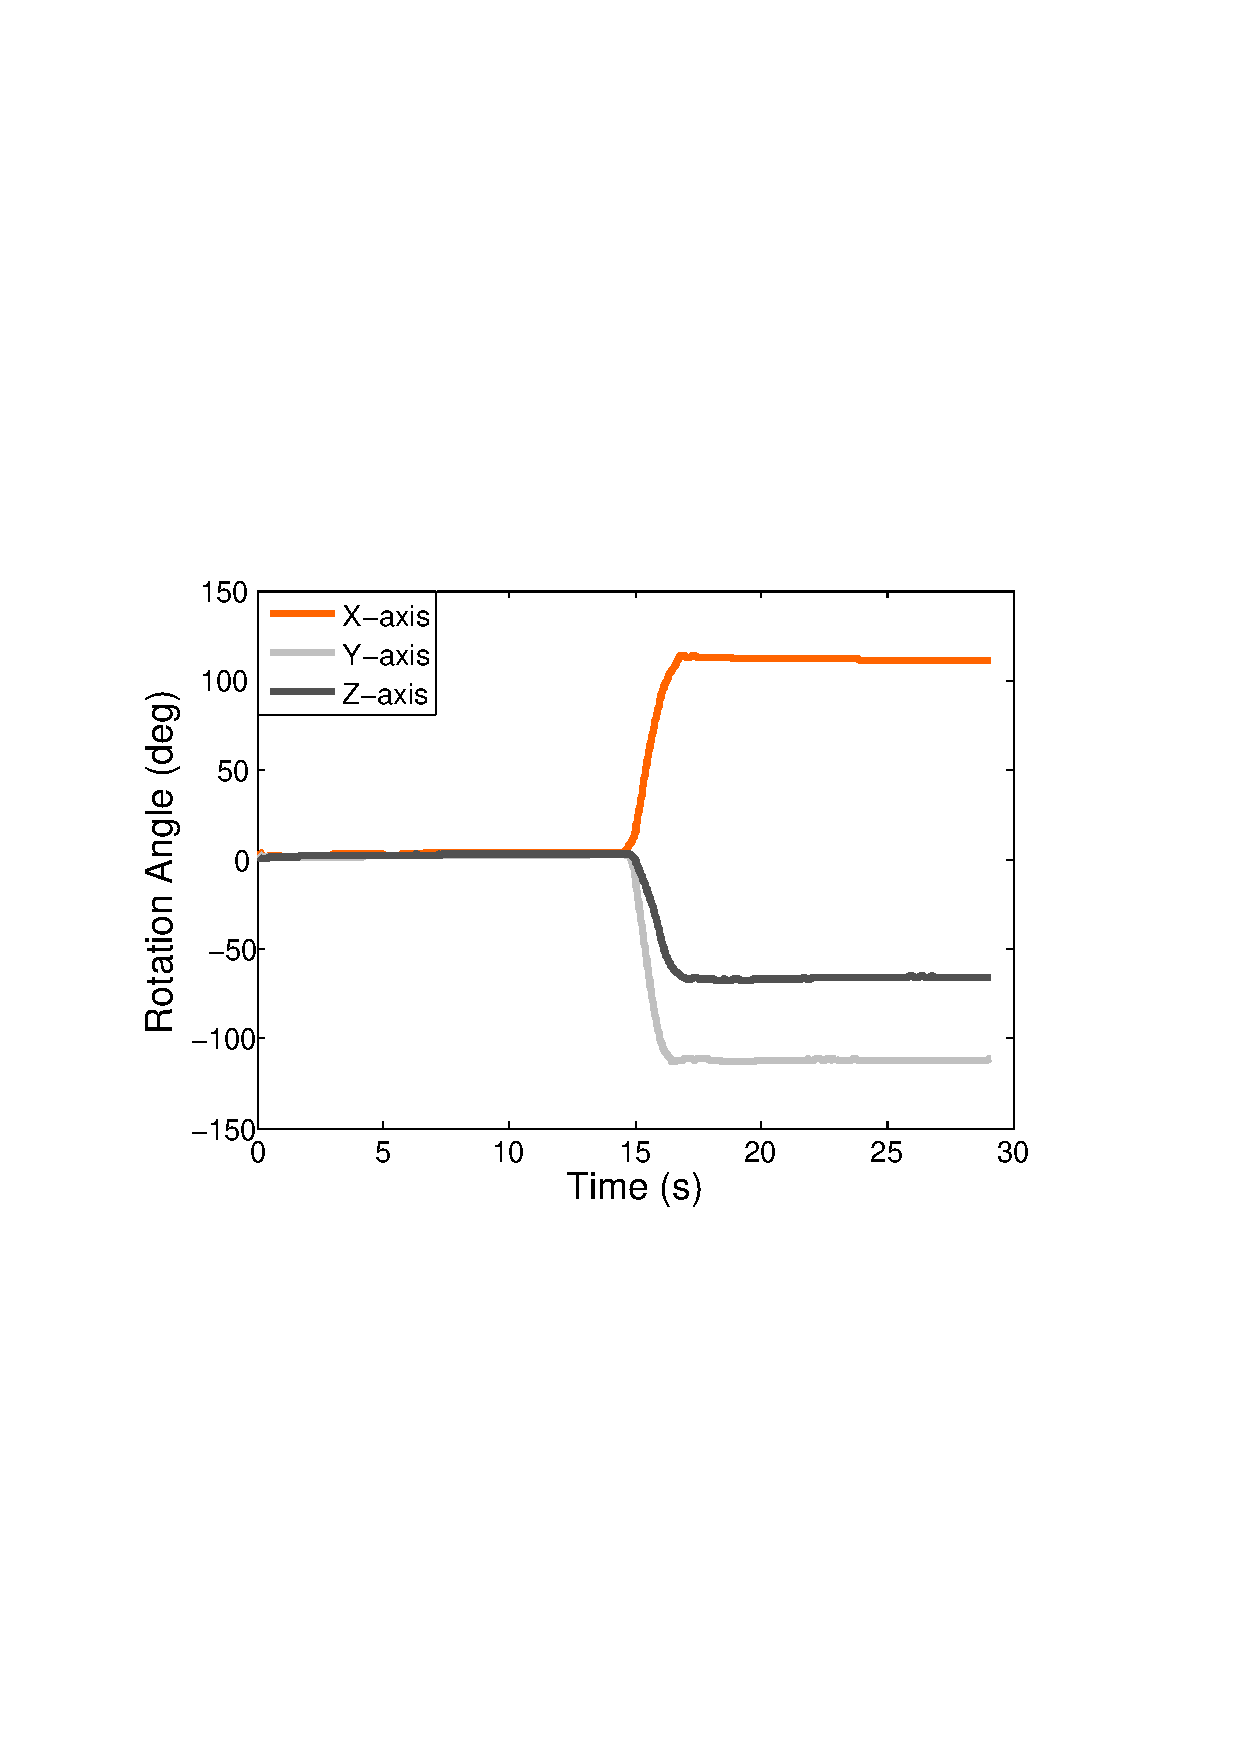
\includegraphics[width=2.7cm,height=2cm]{Figures/BodytoHead.pdf}}
   \caption{The characteristics of hand movement from the position beside the body  to (a)  the abdomen,  (b) the chest, and (c) the head.}\label{Bodyhand}
\end{figure}

\begin{figure}[!t]
\centering
      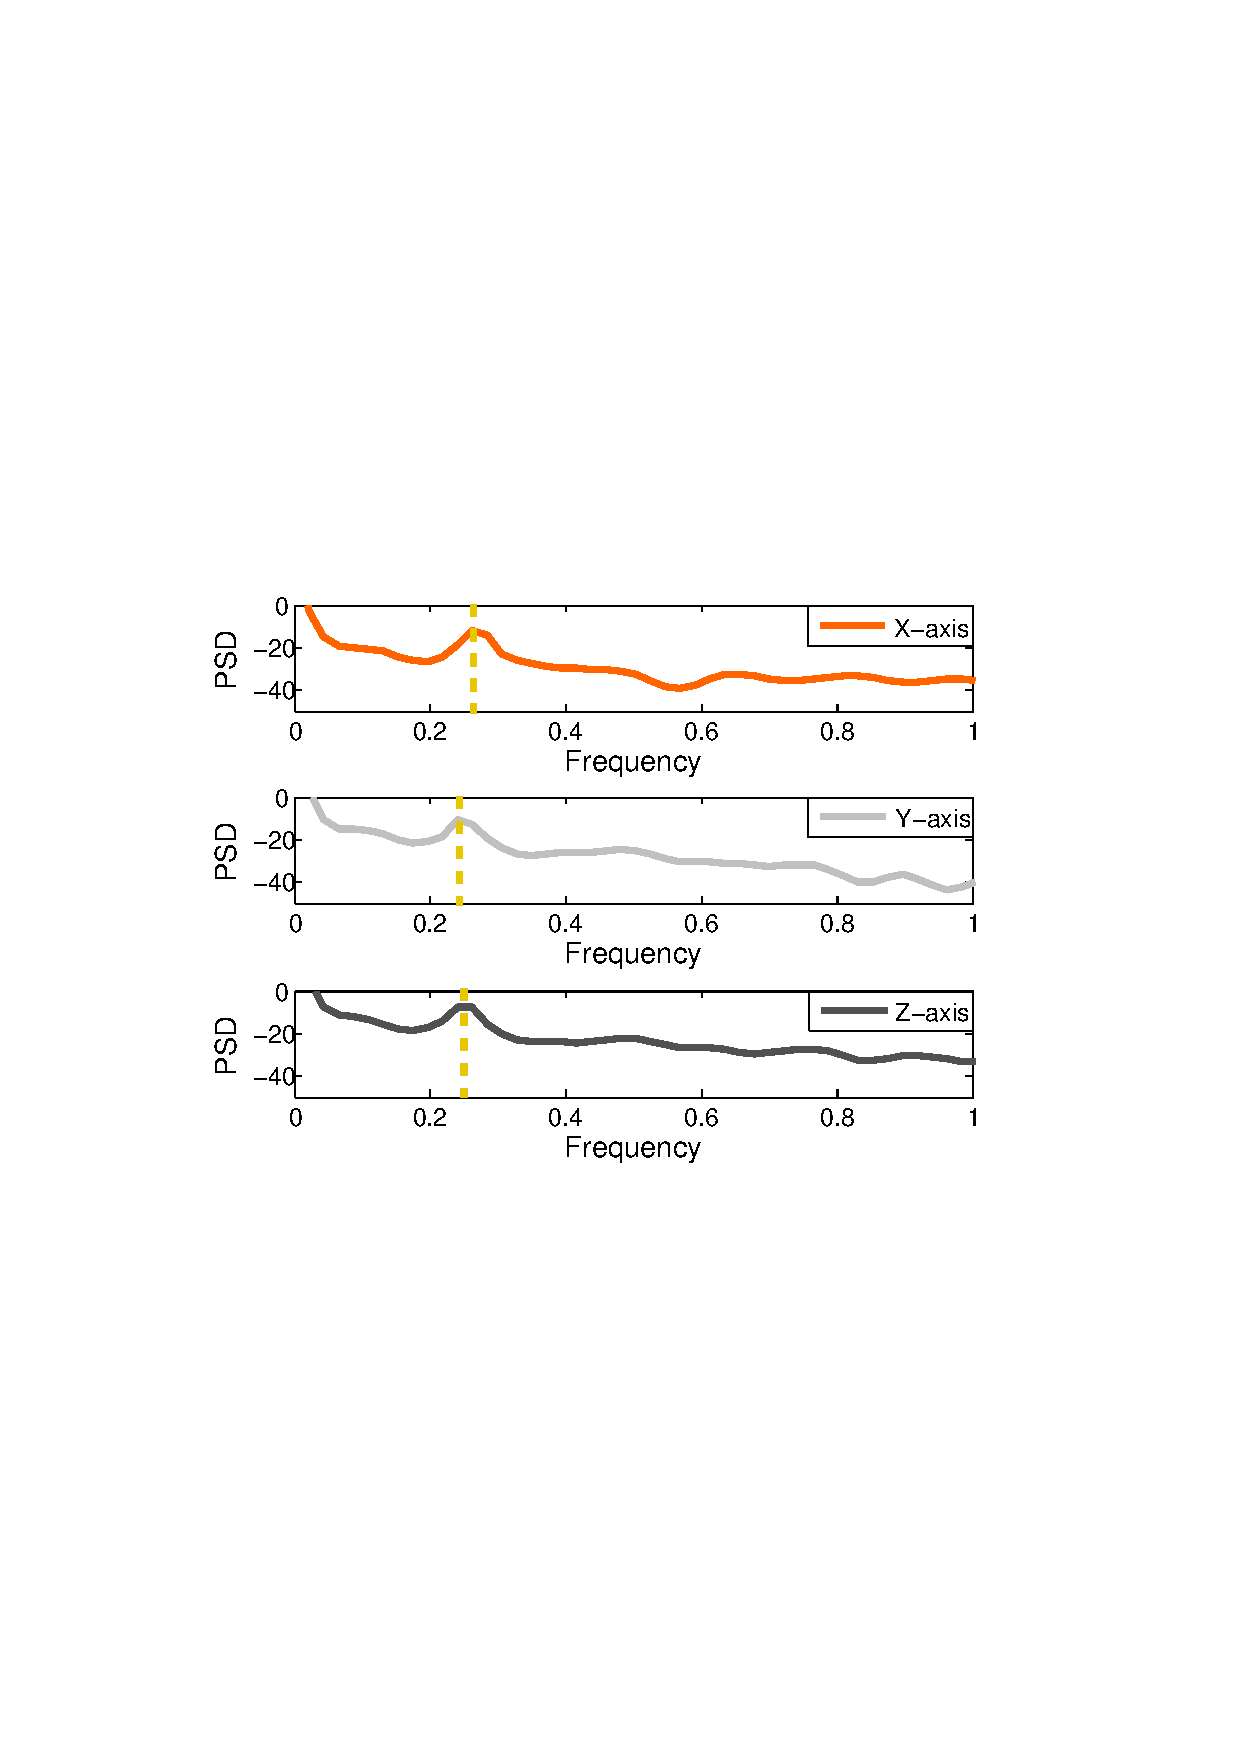
\includegraphics[width=0.77\linewidth]{Figures/PSD.pdf}
  \caption{The power spectral density (PSD) of the acceleration signal.}\label{fig:PSD}
\end{figure}

\begin{figure}[!t]
\centering
      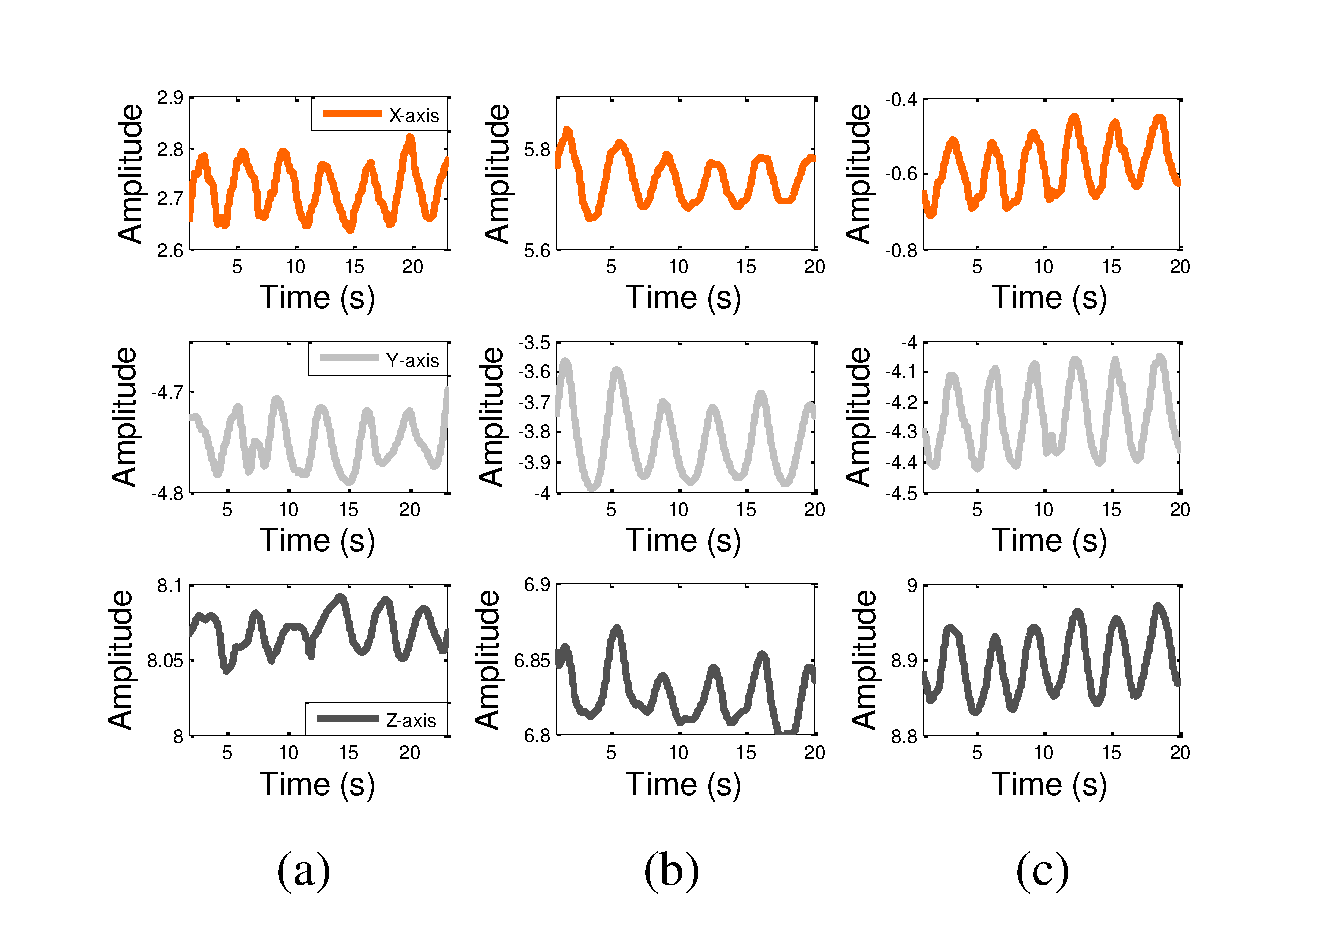
\includegraphics[width=0.77\linewidth]{Figures/breath_ok1.pdf}
  \caption{The periodic change of the acceleration signal. (a) REM--Location 1. (b) REM--Location 2.  (c) NREM--Location 1.}\label{fig:breath_ok1}
\end{figure}

In detail, we found that even the abdomen position, due to the specific location of user's hand put a little different every time, it makes the position of the smartwatch is different, the intensity of the acceleration fluctuation caused by respiration along each axis may be different, so we can not use the direct measured amplitude information to determine respiratory amplitude, as shown in Fig. \ref{fig:breath_ok1}, (a) and (b) are triaxial accelerations at different locations of the abdomen during REM sleep stage, and (c) is the acceleration data of NREM sleep stage at the approximate position in (a). We can see that when hand on the abdomen, but the location is different, even in the same location, we can not directly judge the respiration amplitude using only the amplitude of the three axis of the acceleration.

\begin{figure}[!t]
\centering
      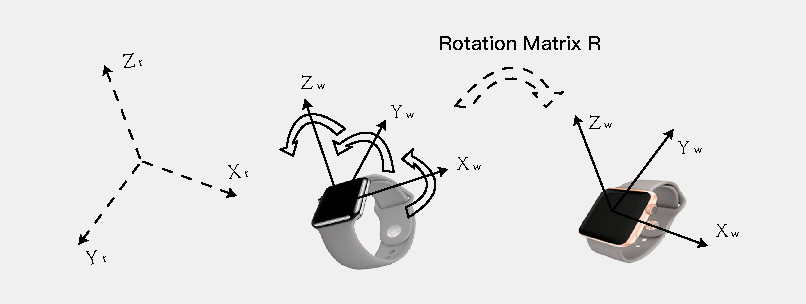
\includegraphics[width=0.87\linewidth]{Figures/watch.pdf}
  \caption{The first figure on the left is the body coordinate system, and $Y_t$ points north. The middle figure shows the watch coordinate system when the watch an arbitrary position, and the right of the figure shows that the  watch coordinate system after we completed the coordinate system conversion.}\label{fig:watch}
\end{figure}

In order to solve this problem, we decided to convert the acceleration data based on the wristwatch coordinate system into the data in the torso coordinate system. Because we can know that when the person is in the supine position, the abdomen and the chest will move up and down due to breathing, that is, move along the z-axis direction of the torso coordinate system. We express the triaxial acceleration data as $Acc_w$ = [$X_w$, $Y_w$, $Z_w$] in the wristwatch coordinate system and $Acc_t$ = [$X_t$, $Y_t$, $Z_t$] in the torso coordinate system, as shown in Fig. \ref{fig:watch}. And the watch coordinate system ({[$X_w$, $Y_w$, $Z_w$]}) is determined by the position of the watch. Our coordinate alignment aims to find a rotation matrix R to align the watch��s coordinate system to the torso coordinate system ({[$X_t$, $Y_t$, $Z_t$]}) and R can be obtained by the three-axis direction information in the orientation sensor. After the coordinate system is aligned, the angle between the y-axis of the wristwatch coordinate system and the y-axis of the torso coordinate system is 180 degrees.

\begin{equation}
      X_��=(X_w\cos\gamma + Y_w\sin\gamma)\cos\theta + (Y_w\cos\sigma + Y_w\sin\sigma)\sin\theta,
\end{equation}
\begin{equation}
      Y_��=-((Y_w\cos\sigma + Y_w\sin\sigma)\cos\theta - (X_w\cos\gamma + Y_w\sin\gamma)\sin\theta),
\end{equation}
\begin{equation}
      Z_��=(Z_w\cos\gamma - Z_w\sin\gamma)\cos\theta - (Z_w\cos\gamma - Z_w\sin\gamma)\sin\theta,
\end{equation}

$\theta$, $\sigma$ and $\gamma$ are the x, y and z axis data of the orientation sensor respectively, representing the direction angle, the tilt angle and the roll angle collected from the orientation sensor. After the alignment of the coordinate system, we can see from Fig. \ref{fig:cordi} that the z-axis shows a periodic signal with significant fluctuations, while the x- and y-axis data undergo smaller changes around zero, which is consistent with the actual situation that when the person is in the supine posture with the abdomen up and down caused by respiratory.

 \begin{figure}[!t]
\centering
      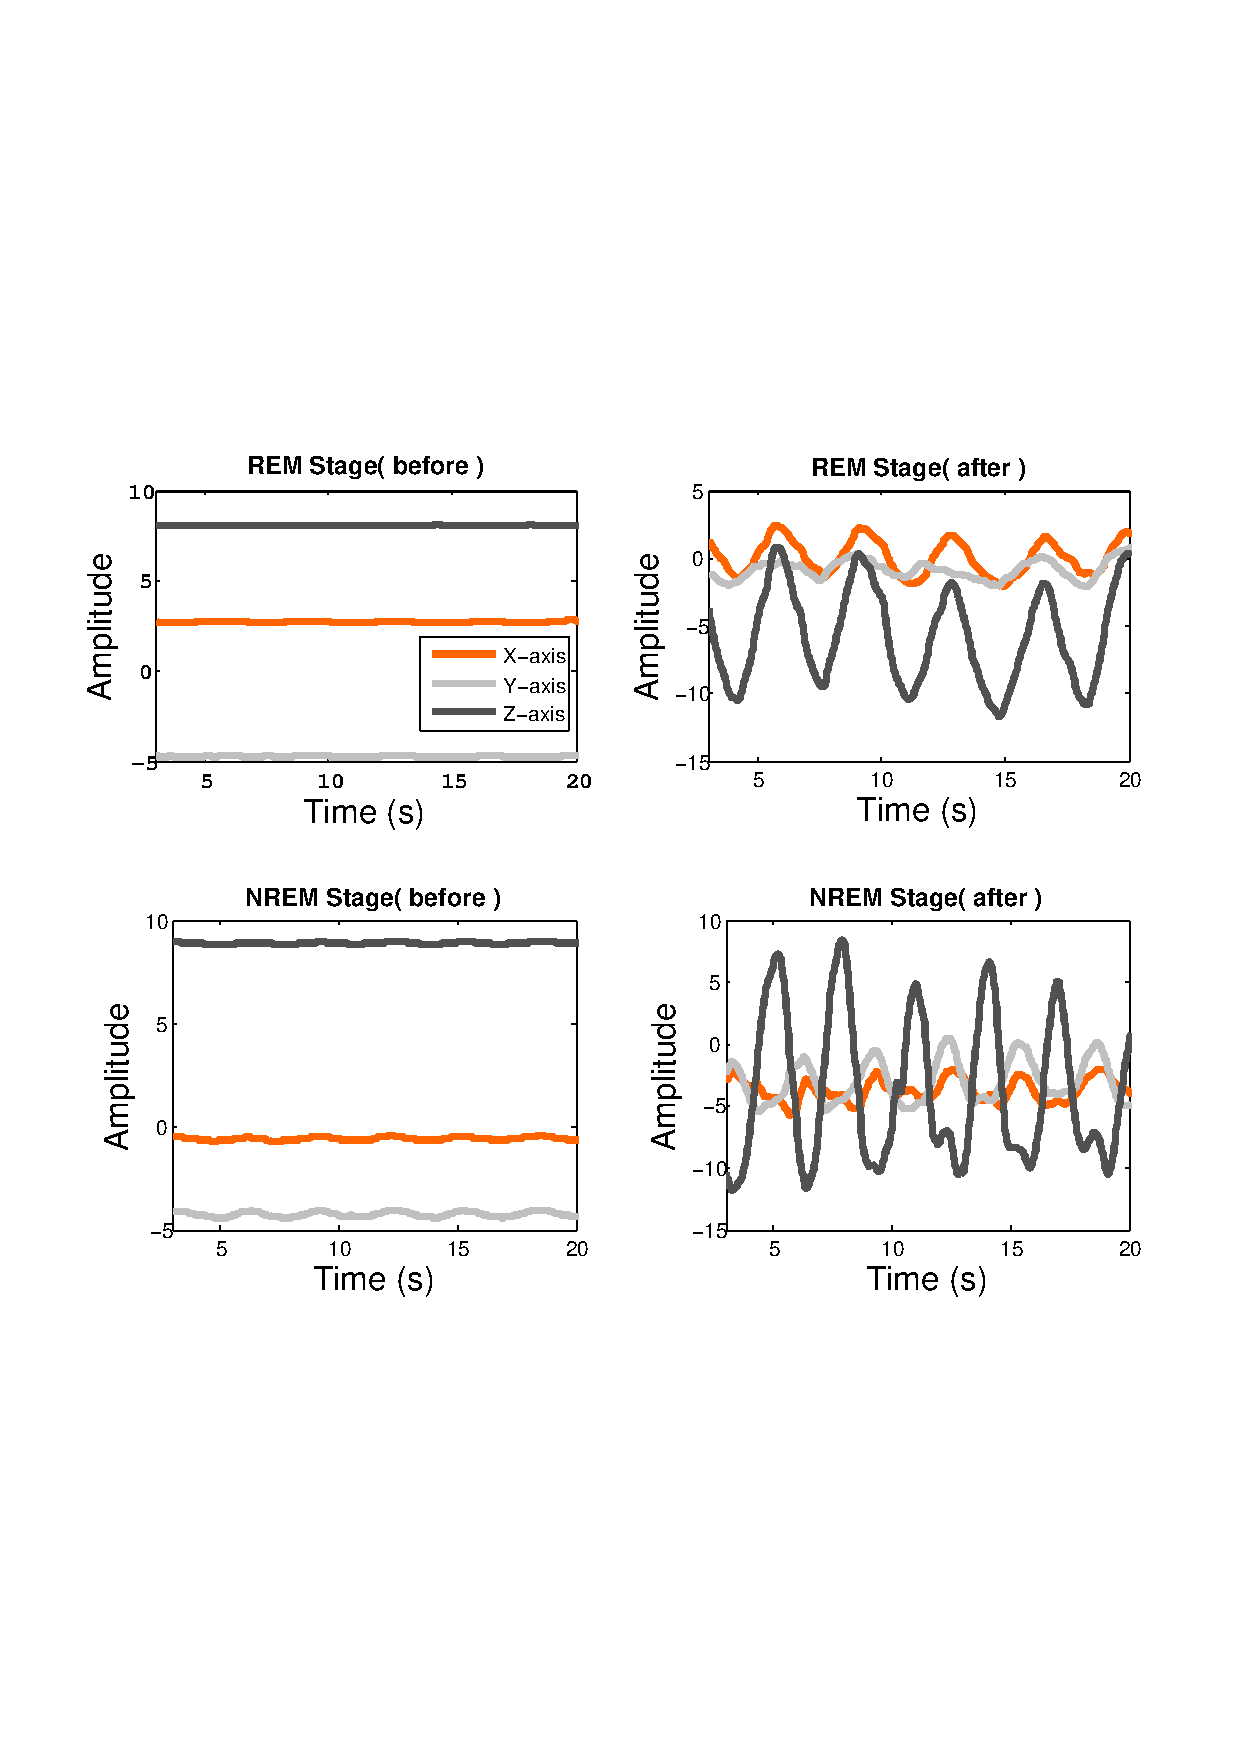
\includegraphics[width=0.77\linewidth]{Figures/cordi.pdf}
  \caption{Acceleration data for different sleep stages.}\label{fig:cordi}
\end{figure}

The two graphs on the left in Fig. \ref{fig:cordi} show the acceleration data in (a) and (c) in Fig. \ref{fig:breath_ok1}, respectively, and the two graphs on the right are these data after the conversion of the coordinate system. We can see that before the alignment of the coordinate system, we can not effectively distinguish between REM stage and NREM stage respiratory amplitude from the acceleration amplitude, but after the coordinate system alignment, we can judge the amplitude from the z-axis data well. Here, we choose to calculate the amplitude variances of the z-axis acceleration as a feature, it can be used to measure the intensity of the fluctuation in a signal and a larger variance means that the greater the amplitude of the breaths. Therefore, we further train the variance of the acceleration data when the hand on the abdomen and on the chest under the REM stage and the NREM stage to determine the current respiratory amplitude. We trained 200 sets of acceleration data (100 sets of these from the larger respiratory amplitude and the rest of sets from the normal respiratory amplitude ) from 10 volunteers. Eventually, we concluded that the variance threshold for the acceleration data is 15 when the hand on the abdomen, and the variance threshold is 4 when the hand on the chest.


 \begin{figure}[!t]
\centering
      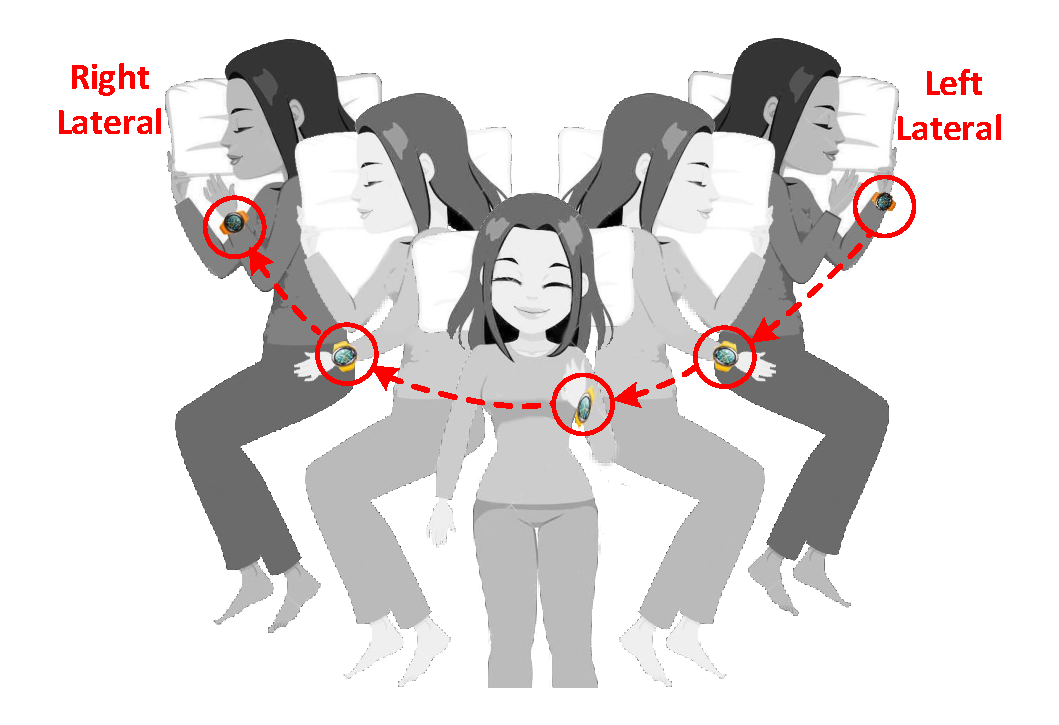
\includegraphics[width=0.47\linewidth]{Figures/BodyRollover.pdf}
  \caption{Body rollover from the left side to the right side.}\label{fig:BodyRollover}
\end{figure}


\subsubsection{Body rollover counts}
Under normal circumstances, people usually body rollover about 20-45 times a night, the meaning of body rollover is to maintain a comfortable position. Otherwise, for a long time to maintain a sleep posture, some muscles will be in a state of tension, making the body in contact with the bed due to oppression caused by poor blood supply, nerve compression will lead to local numbness \cite{rollover2014}. So body rollover is another key indicator about the sleep quality. {\systemname} can detect the number of body rollovers, which can get some reflections of sleep status and the roll-over frequency can also help us to classify the sleep stage \cite{rollover2007}. In general, there are six cases: four posture transition cases between the supine posture and lateral (left or right) posture, and two posture transitions between the left lateral posture and right lateral posture. Fig. \ref{fig:BodyRollover} shows the case when the body moves from the left side to the right side. When the rollover occurs, we observe different change patterns about the tilt angle values. Specifically, the angle values of three different axes are on the falling edge or rising edge simultaneously during a very short time period. Fig. \ref{fig:LeftToRight} -- Fig. \ref{fig:RightToLeft} shows the value changes under different body rollover cases. To this end, one straightforward method to detect the rollover is to test the angle value changes. However, this method suffers a very large error since other hand movements will also induce a similar data changes.

\begin{figure*}[!t]
%\centering
%   \setlength{\abovecaptionskip}{-2pt}
% \setlength{\belowcaptionskip}{-9pt}
\begin{minipage}[t]{0.31\linewidth}\centering
    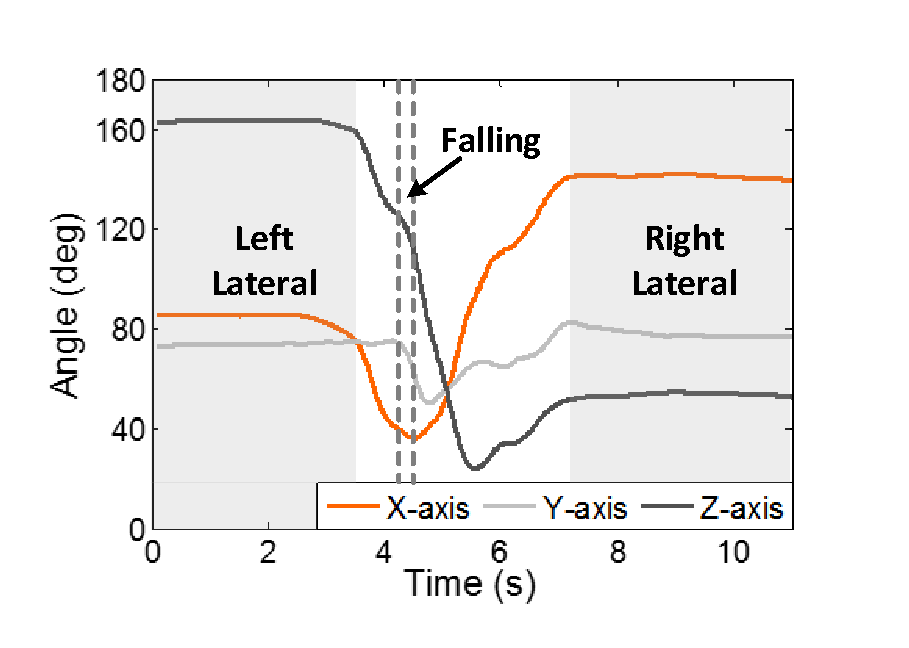
\includegraphics[width=0.87\linewidth,height=3.7cm]{Figures/LeftToRight.pdf}\centering
  \caption{From left lateral posture to right lateral posture.}\label{fig:LeftToRight}
\end{minipage}
\hspace{2pt}
\begin{minipage}[t]{0.31\linewidth}\centering
    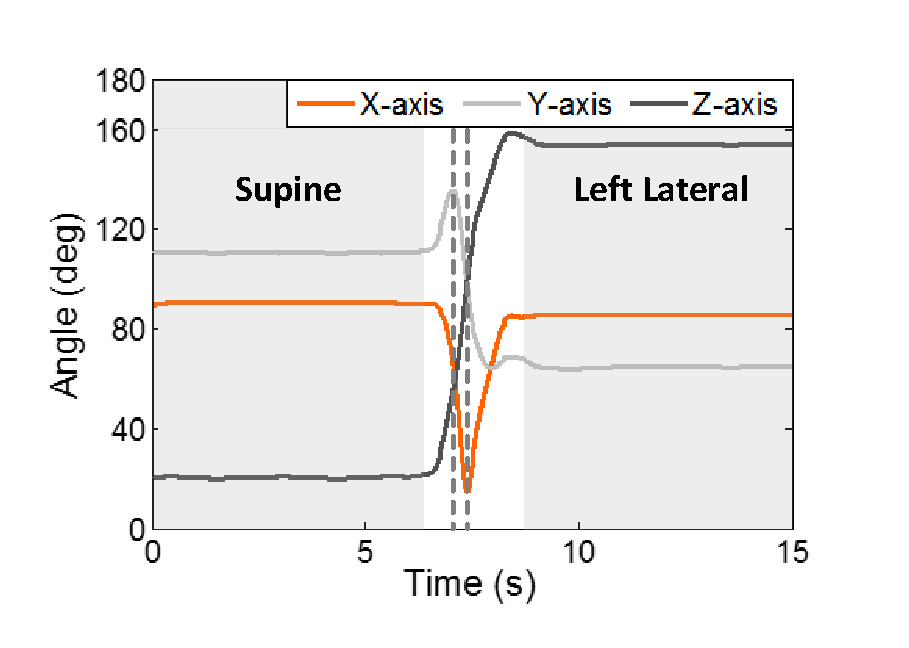
\includegraphics[width=0.87\linewidth,height=3.7cm]{Figures/SupineToLeft.pdf}\centering
  \caption{From supine posture to left lateral posture.}\label{fig:SupineToLeft}
\end{minipage}
\hspace{2pt}
\begin{minipage}[t]{0.31\linewidth}\centering
    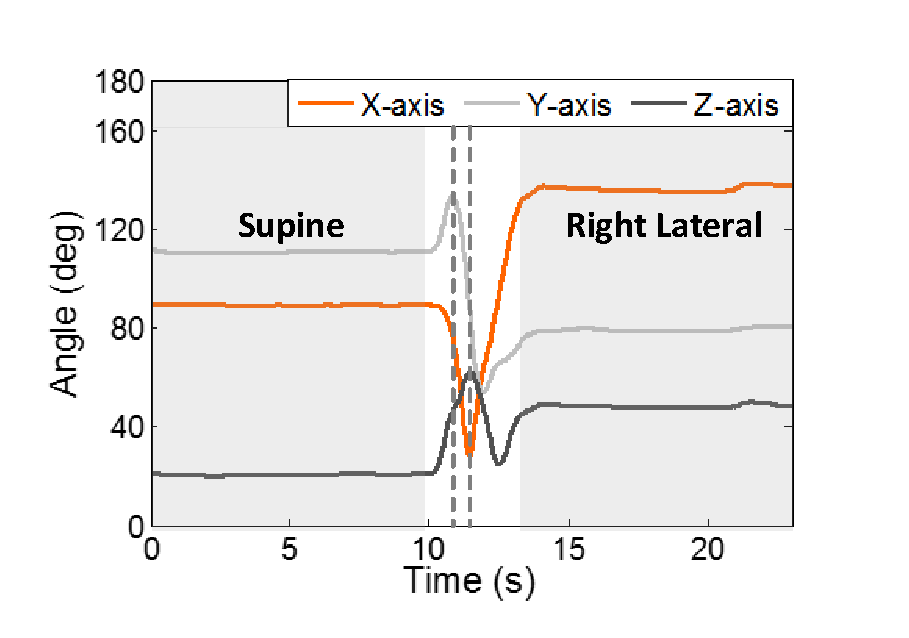
\includegraphics[width=0.87\linewidth,height=3.7cm]{Figures/SupineToRight.pdf}
  \caption{From supine posture to right lateral posture.}\label{fig:SupineToRight}
\end{minipage}
\hspace{5pt}
\begin{minipage}[t]{0.31\linewidth}\centering
    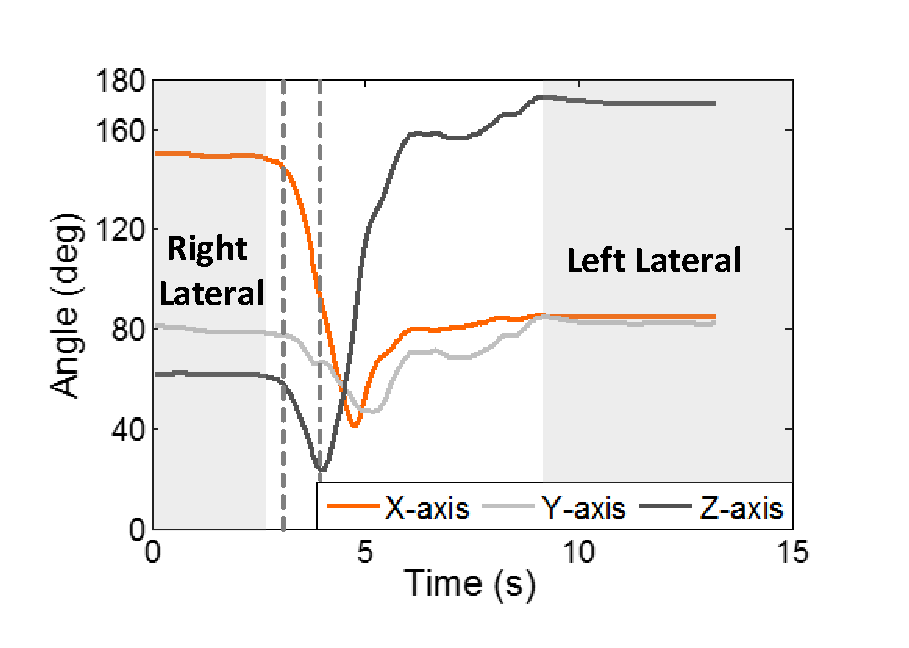
\includegraphics[width=0.87\linewidth,height=3.7cm]{Figures/RightToLeft.pdf}
  \caption{From right lateral posture to left lateral posture.}\label{fig:RightToLeft}
\end{minipage}
\hspace{12pt}
\begin{minipage}[t]{0.31\linewidth}\centering
    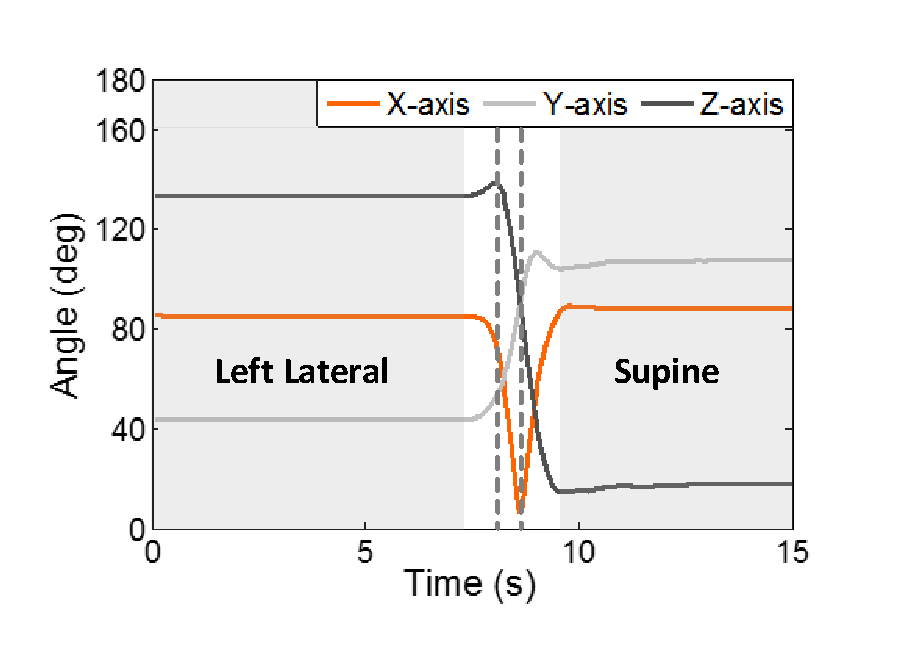
\includegraphics[width=0.87\linewidth,height=3.7cm]{Figures/LeftToSupine.pdf}
  \caption{From  left lateral posture to supine posture.}\label{fig:LeftToSupine}
\end{minipage}
\hspace{16pt}
\begin{minipage}[t]{0.31\linewidth}\centering
    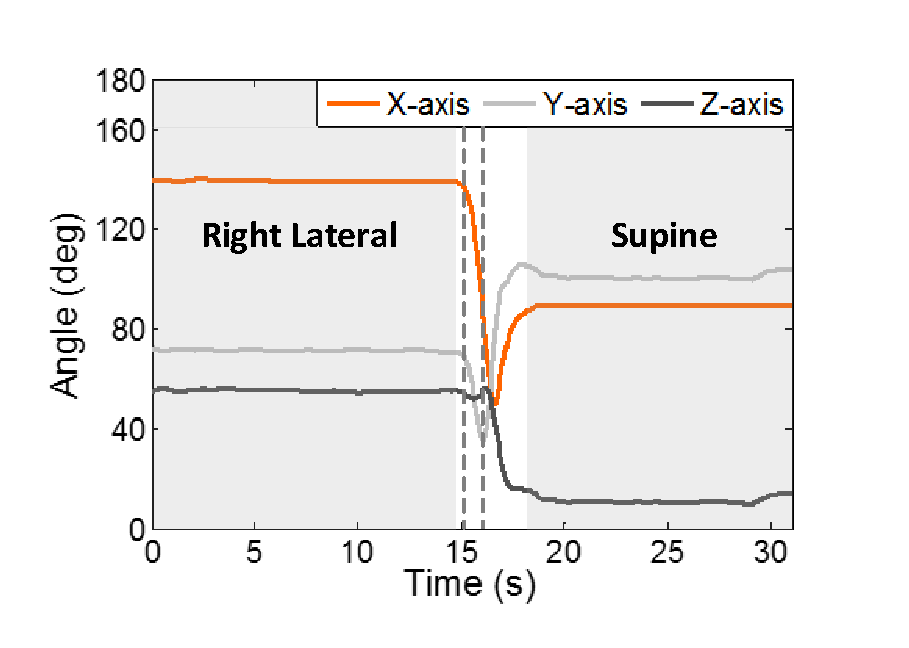
\includegraphics[width=0.87\linewidth,height=3.7cm]{Figures/RightToSupine.pdf}\centering
  \caption{From right lateral posture to supine posture.}\label{fig:RightToLeft}
\end{minipage}
\end{figure*}

To deal with this challenge, we incorporate the body postures to improve the detection accuracy. As shown in Fig. \ref{fig:BodyRollover}, the body postures are different before and after the rollover. Therefore, after we detect the time when the angle values changes, we term the time as a possible rollover time point. Then we use the sleep posture classification algorithm to determine whether the body postures are the same or not over a period of time before and after this point. If the postures are different, we exclude this time point, otherwise the system detects a body rollover event. Note that {\systemname} can not only count the number of rollovers, but also report the detailed rollover event.


\subsubsection{Micro body movement}
Except for the large body movement like rollover, there are some involuntary body movements. With the deepening of sleep, limbs are extremely relaxed, and a little stimulus will produce trembling and micro beating. Such behavior is most likely to occur during the deep sleep stage and the REM stage \cite{ancoli2003role,Jean2000Sleep}. Therefore, by detecting such micro body movements and distinguish them from large body movements can help us to further analyze the user's sleep stage. In this paper, we are interested in the sleep-related body movements including hand moving, arm raising, and body trembling.

The way of detecting micro movement is different from the method of detecting the body rollover, we first need to consider the influence of inherent accelerometer��s noise. In addition to the appropriate data preprocessing, we need to set an appropriate threshold to classify the accelerations of micro body movements and noises. To set an effective threshold, we conduct extensive experiments across 10 volunteers. In each experiment, the volunteer is asked to wear a smartwatch and enables the accelerometer embedded in smartwatch to calculate the corresponding acceleration variance trace of the micro body movement. we smooth the acceleration along the three axes using Moving Average filter, and calculate Root Sum Square (RSS) to merge them.
\begin{equation}
      Rss(t)=\sqrt{(acc_x(t))^{2}+(acc_y(t))^{2}+(acc_z(t))^{2}},
\end{equation}
$acc_x(t)$, $acc_y(t)$ and $acc_z(t)$ represent the accelerometer sample value of x-axis, y-axis and z-axis at time stamp t respectively. And then we can obtain the acceleration variance.
\begin{equation}
      V(t)=Rss(t)-Rss(t-1).
\end{equation}

Eventually,we set the threshold to be 0.03, which can achieve a satisfactory detection performance. We also observe that the micro-movement duration is very short, which lasts less than 2 s. However, in our body rollover experiments, we find that the average movement duration is 3 s, as shown in Fig. \ref{fig:LeftToRight} - Fig. \ref{fig:RightToLeft}. Therefore, we can first divide the body movement events into large movement and micro movement by detecting the signal duration time. Then for the micro body movement events including hand movement, arm raising and body trembling, we first find that the durations of these movements are significantly different. The average duration of arm rising is 1.8 s, but the duration of hand movement is only 1 s, what��s more, the body trembling lasts less than 1s, as shown in Fig. \ref{fig:micro-move}. The temporal gap is so obvious that we can easily distinguish the arm raising and the other two movements. In order to further classify the hand movement and body trembling, we observe the corresponding acceleration variance. As we can see from the figure, the acceleration of body trembling has a more pronounced peak when compared to the hand movement. So we perform peak detection on the acceleration variance. For the detected peak, we calculate the difference $d$ between this peak and the average of the peaks in the reference data set.
\begin{equation}
      d=\mid(peak-average(oi))\mid,
\end{equation}
$oi$ indicates the type of micro-movement, when $oi$ is 1, it indicates the hand movement and 2 represent body trembling.


\begin{figure}[!t]
\centering
      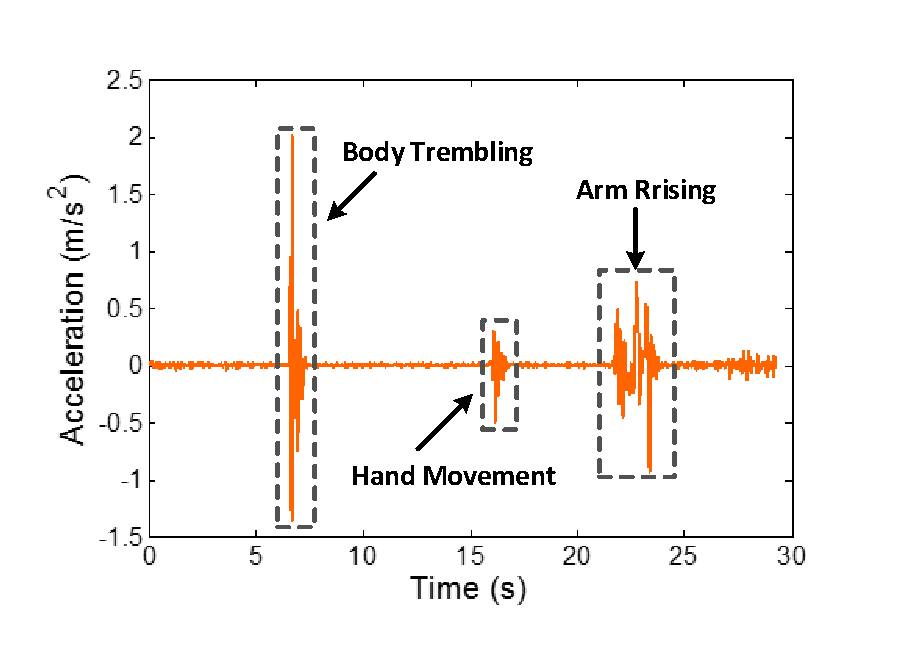
\includegraphics[width=0.47\linewidth]{Figures/Micromovement.pdf}
  \caption{Acceleration reading for micro body movements.}\label{fig:micro-move}
\end{figure}

For the two types of potential micro-movements to be classified, we calculate variances for 100 sets of micro-movement data for these 10 volunteers and perform peak detection, as well as make these peaks as features for a particular type of movement to establish a reference data set. In order to classify the micro-movement more accurately, we further obtain the average of the peak features ($average(oi)$) in the reference data set. And then we determine the type of micro-movement with the smallest value of d as the final detection result.


\subsection{Acoustic Event}
Acoustic events during sleep, such as snore, cough and somniloquy, can reflect and affect user's sleep quality and physical health. For example, snore is one of the possible symptoms of cerebral infarction patients.  And long-term snoring can also have a serious impact on health and sleep. It can cause behind sleep apnea or narcolepsy, a sleeping disorder \cite{snoring2016,snoring2013}. And when there is a cough, the human cerebral cortex cells are always in an excited state, limiting the depth of sleep, allowing only short sleep between wakefulness, like many other sleep disruptions. {\systemname} can detect these different acoustic events, including snore, cough and somniloquy. Different from traditional parameters based acoustic classification algorithm \cite{gu2016sleep}, we exploit the inherent characteristics of different acoustic events and design a lightweight algorithm for effective classification.

\begin{figure*}[!t]
\centering
%   \setlength{\abovecaptionskip}{-2pt}
% \setlength{\belowcaptionskip}{-9pt}
%\begin{minipage}[t]{0.32\linewidth}\centering
 \subfigure[Snore of six times.]{\label{snore}
   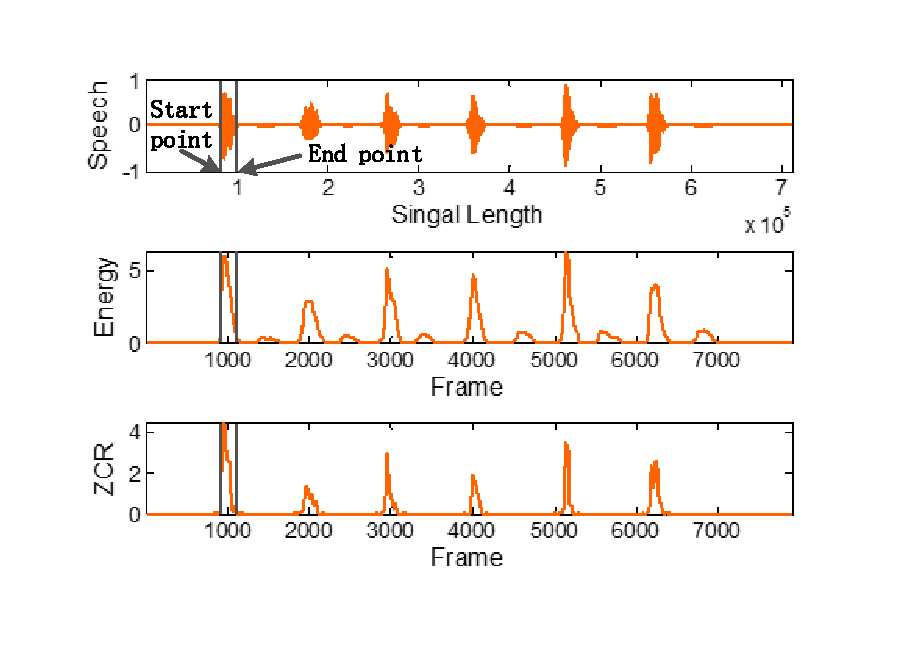
\includegraphics[width=0.325\linewidth]{Figures/snore.pdf}}
 \subfigure[Two consecutive cough.]{\label{cough}
   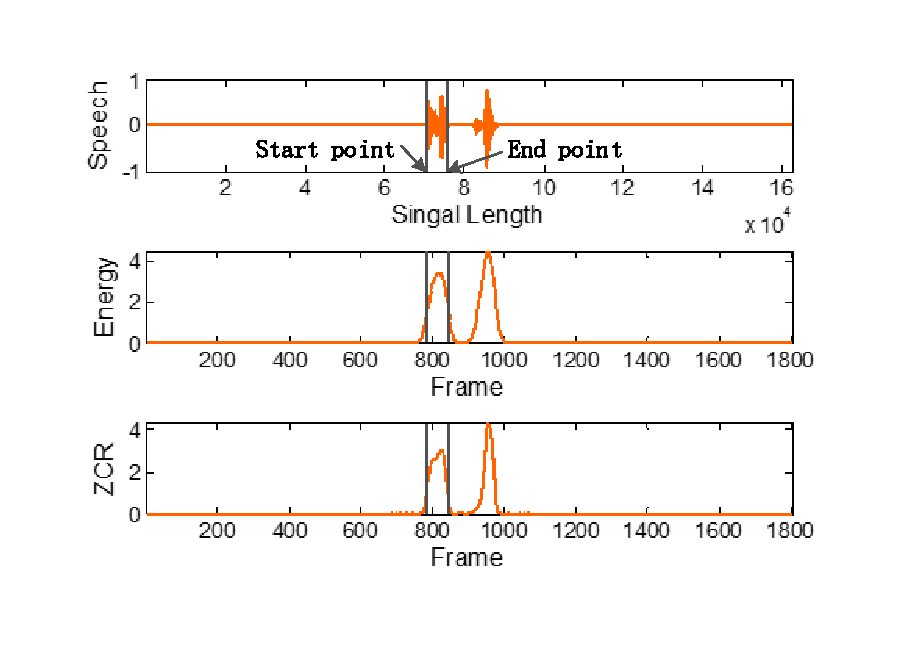
\includegraphics[width=0.325\linewidth]{Figures/cough.pdf}}
\subfigure[Somniloquy.]{\label{somniloquy}
     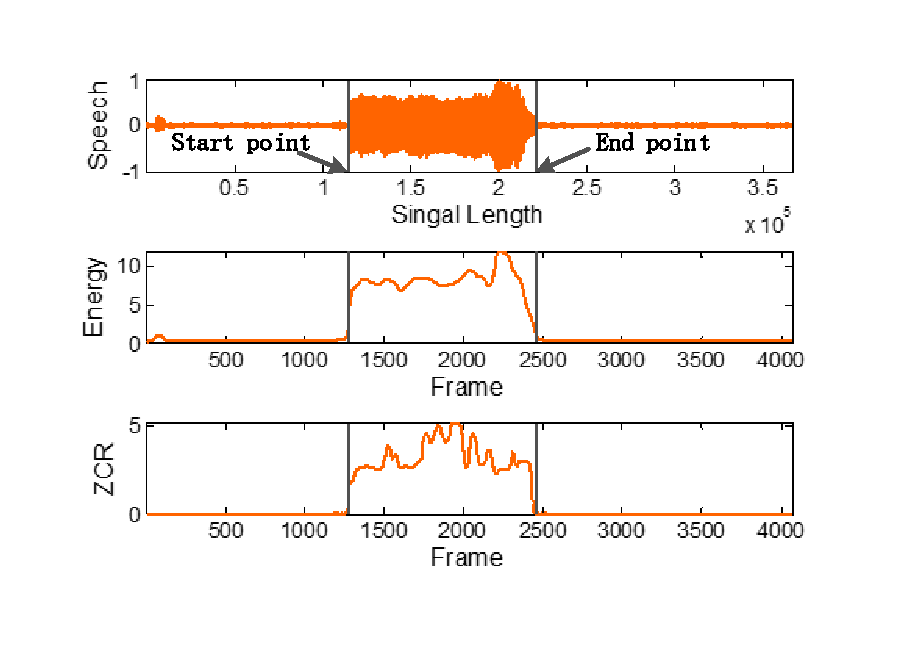
\includegraphics[width=0.325\linewidth]{Figures/somniloquy.pdf}}
\caption{The characteristics of different acoustic events.}\label{acoustic}
\end{figure*}


\textcolor{blue}{\subsubsection{Acoustic feature calculation}}
In order to identify different acoustic events accurately, we select the short-term average energy and the zero-crossing rate as two features. The short-term average energy of acoustic signal is computed as:
\begin{equation}
  E_i=\sum\nolimits_{j=-\infty}^{\infty}[x(j)\omega(i-j)]^2=\sum\nolimits_{j=i-(N-1)}^{i}[x(j)\omega(i-j)]^2,
\end{equation}
$N$ is the window length. As we can see that the short-term energy is the weighted sum of squared frame sample. The short-term energy can be used to distinguish the segment of unvoiced and voiced sound. It also can be used to differentiate speech segment and noise segment  in  case of relatively high signal to noise ratio (SNR). The zero-crossing rate is computed as:
\begin{equation}
  Z_i=\frac{1}{2}\sum\nolimits_{j=0}^{N}|sgn[x_i(j)]-sgn[x_i(j-1)]|.
\end{equation}
It indicates the number of times, which the acoustic signal waveform passes through the horizontal axis (zero level). We carry out an interesting recognition experiment using the microphone built in smartwatch to detect the sound of people during sleep and effectively identify different acoustic events. We focus on three common acoustic events: snore, cough and somniloquy. Ten volunteers worn the smartwatches during sleep to record the acoustic data. We manually label the data with different acoustic events. Fig. \ref{acoustic} shows the acoustic characteristics of  three events. There are six times snore event, two consecutive cough event and somniloquy event.
%The sample rate is 22050 Hz.


\textcolor{blue}{\subsubsection{Acoustic event recognition}}
 At beginning, the algorithm  divides the audio stream into frames with equal durations. Each frame is composed of 256 samples, and its duration is 12 ms. To identify the  three common acoustic events, we introduce an acoustic recognition algorithm based on the following key observations:

 \begin{itemize}[itemsep=1mm,nolistsep]
\item The time interval between two signals for different acoustic events are quite different from each other. As shown in Fig.~\ref{snore}, there is a long time interval between two snores. While, the time interval between two coughs is very short.  In contrast, the  somniloquy signal is irregular and without periodic property.
    %Besides, the snore event produces periodic signals and their intervals  are similar.
 \item The duration of one signal for different acoustic events are different from each other. Fig. \ref{acoustic} shows that the duration of a snore is shorter than the duration of a cough and somniloquy. And in general, the duration of a cough is shorter than the duration of a somniloquy signal.
\item The frequencies for different acoustic events are quite different from each other. Snore event has a continuous signal, while the  cough and somniloquy are sudden events, thus the number of consecutive occurrences is very small.
\end{itemize}
In conclusion, the ``interval'', ``duration'' and ``frequency'' of acoustic events can be used as three unique features. Based on the above three observations, our acoustic event recognition algorithm involves the following two steps. First, in order to estimate the interval and frequency of a acoustic event, we perform the peak detection. We use the short-term average energy to calculate the peak value of the acoustic signal. When the peak exceeds a certain threshold, such as 3 dB in this paper, we record the position of each peak and calculate the interval between two consecutive peaks. Next, we can estimate the frequency of a acoustic event by counting the number of peaks over a time window. Second, to estimate the duration of the acoustic event, we perform the start-point and end-point detection.

Traditional end-point detection algorithm \cite{stowell2015detection}, however, uses a fixed double threshold and must be obtained by a large number of data samples, which has two drawbacks. First, the fixed double threshold may cause error detection at the beginning of acoustic event. Second, the requirement of a large number of data samples would lead to large system latency. To deal with those problems, we introduce an improved end-point detection method, which improves the detection accuracy and reduces the number of data samples. The proposed method has a adaptive threshold, in detail, Since the first few frames and the last few frames are mostly mute or background noise, we select the first five frames and the last five frames to calculate their short-term energy, which are denoted as $Es$ and $Ee$, respectively. And then the two are combined to obtain the mean $En$ as the estimated energy value of the noise segment.Let the maximum value of the short-term energy over all frames denoted as $\max (E)$. Then, the average short-term energy $DE$ is given as:
\begin{equation}
      En=\frac{(Es+Ee)}{2},
\end{equation}
\begin{equation}\label{eq:DE}
      DE=\max (E)-En.
\end{equation}

So we can use $EH$ and $EL$ to represent the high and low threshold of short-term energy, which are given as:
\begin{equation}
      EH=0.1\times DE+En,
\end{equation}
\begin{equation}
    EL=0.06\times DE+En,
\end{equation}

 As a result, we can reduce the number of data samples required for detection. Moreover, in order to avoid the interference of sudden noise, we set the minimum length of the signal segment and count the length of the signal during the search for the start and end point. Finally, if the signal length is less than the set minimum, it is considered as a noise segment. The results of the start-point and end-point detection are shown in Fig. \ref{acoustic}, we calculate the length of each speech segment and calculate their averages as the duration of the acoustic event. Last, we count the number of peak points to determine whether it meets the third key observation or not.



%Algorithm 1 provides the detailed  process of the start-point  and end-point detections.


%$A_x$, $A_y$ and $A_z$ are the tilt angle of the three axes, and $\omega_x$, $\omega_y$ and $\omega_z$ are the rotation speed of the three axes. So $\phi$, $\theta$ and $\psi$ are the rotation angle of the three axes. \textcolor[rgb]{1.00,0.00,0.00}{(Those symbols do not present in Algorithm 1)}


%\begin{table}[!thbp]
%\begin{tabular}{l}
%  \hline
%  \textbf{Algorithm 1} The Endpoint Detection \\
%  \hline
%  \textbf{Input}: A sound signal recorded by the microphone:$x$
%  \\\quad \quad \quad The threshold of zero-crossing rate:$ZT$
%  \\\quad \quad \quad The minimum length of speech:$minlen$\\
%  \textbf{Output}:The start-point  and end-point :$p_s,p_e$\\
%  1: Split  $x$ using the framing algorithm \\
%  2: Calculate each frame of energy and zero-crossing rate:$E_i,Z_i$ \\
%  3: Calculate the threshold for short-time energy:$EH,EL$  \\
%  4:$count=0$,$silence=0$\\
%  \textbf{the start point}\\
%  5:\textbf{for}i=1$\rightarrow \frac{length(x)}{frame~length}$  do\\
%  6: \textbf{if} $ E_i>EH $ \textbf{then}\\
%  7: $count=count+1$,$silence = 0$,$max(n-count-1,1)=p_s$\\
%  8: \textbf{else if} $E_i>El || z_i>ZT $\textbf{then}\\
%  9: $count=count+1$ \\
%  10: \textbf{else}\\
%  11:$count=0 $ \\
%  12: \textbf{end if}\\
%  \textbf{the end point}\\
%  13:\textbf{if} $E_i>El || z_i>ZT $\textbf{then}\\
%  14:$count=count+1$ \\
%  15:\textbf{else}\\
%  16:$silence = silence+1 $ \\
%  17:\textbf{if} $count < minlen$\textbf{then}\\
%  18:$count=0 $, $silence=0$ \\
%  19:\textbf{end if}\\
%  20:$count1 = count-\frac{silence}{2}$\\
%  21:$ p_e = p_s + count1 -1$ \\
%  \hline
%\end{tabular}
%\end{table}


\textcolor{blue}{\subsection{Illumination Condition}}
Studies have shown that there is a significant interaction between illuminance level and the mental state of the individual \cite{light77}. For example, the bright light can counteract subjective fatigue during daytime, but at night it will seriously affecting the sleep quality. Too much light exposure can shift our biological clock, which makes restful sleep difficult to achieve, it affects our sleep and wake cycle \cite{light2007}.  Besides, we also note that the dim light will affect our sleep too. According to the study \cite{light2016}, it can be learned that the dim artificial light during sleep is significantly associated with the general increase in fatigue, and the proper light can be used to increase the sense of exhaustion and promote sleep. So illumination condition in a sleeping environment have a significant influence on sleep. {\systemname} use the ambient light sensor to detect the illumination condition during sleep. We visit 10 volunteers' bedroom at night and the use of the ambient light sensor to test the lighting conditions in the bedroom, and ultimately we will divide the illumination intensity into two conditions: bedroom without light (Weak illumination condition, $\leq$ 10Lux);  bedroom with strong lights (Strong illumination condition, $>$ 10Lux). Therefore, we can learn the light conditions in the sleeping environment according to the two types of illumination conditions.

However, the light sensor may be obscured, which leads to large errors in measuring the illumination level. For example, a user��s smartwatch may be covered under quilt when he/she turned over unconsciously, and thus the illumination readings on the smartwatch may not reflect the real lighting situation. To deal with this problem, the key is that the illumination would drop suddenly when the smartwatch is covered by other objects. There are two possibilities for the sudden drop in light intensity. For most smartwatches, the light sensors are usually installed in the front face of it. The first case is the indoor lighting facilities are closed. The second case is the wrist turned so that the back of the hand become downward, thus blocking the light sensor in front of the smartwatch. To avoid this erroneous illumination condition measurement, we detect whether the user is performing a wrist flip over a period of time during the intensity plummeting. We detect the wrist flip based on two aspects: (i) the rotation angle of smartwatch; (ii) wether the light intensity maintain stable after the sharp drop. If the wrist flips, we use the average of the previous light intensity as the intensity of the time period. It should be noted that, because the illumination condition detection algorithm is relatively simple, it is not explained in the experimental part.

\subsection{Sleep stage and quality}
Sleep is a cyclical process composed of three stages: rapid eye movement (REM) stage, light sleep stage and deep sleep stage. The entire sleep process can be divided into many sleep cycles, in each sleep cycle, the sleeper first experienced a transition from light sleep to deep sleep, and then enter the REM. However, the sleep stage can also jump from light sleep to REM or deep sleep directly from REM.To estimate the sleep stage, we use the HMM model \cite{johnson2010hidden} since different sleep stages have potential conversion probabilities. Usually, when a user is in different sleep stages, he/she will have different sleep-related activities.For example, a person may roll over in bed when he/she is in light sleep stage, and keep motionless when he/she is in deep sleep stage. And when he/she get into the deep sleep, it will appear snoring, body trembling, etc., in the meanwhile, the breathing amplitude larger than when he/she sleep in the light stage. Thus, based on these features,we use all the detected sleep-related activities as the HMM model input. And we use a series of sleep events as observation sequence, corresponding to the sleep stage as an implicit state sequence, first using maximum likelihood estimation method for parameter estimation, the state transition matrix and the confusion matrix, and then use the Viterbi algorithm \cite{viterbi} can be obtained A series of implicit state sequences corresponding to observed sequences. That is to say that  based on HMM model, we can estimate the sleep stage during a time window, such as 2 hours. Finally, we can get the durations of all sleep stage over the whole sleep process.

Further, to quantize the quality of a sleep, we use the Sleep Quality Report model introduced in \cite{gu2016sleep}. Let $SQ$ be the value of the sleep quality, then $SQ$ is given as follow:
 \begin{equation}
SQ=\frac{(REM \times 0.5+Light \times 0.75+Deep) \times 100}{REM+Light+Deep}
 \end{equation}
where, REM, Deep and Light represents the duration time in a sleep process. The range of $SQ$ is from 50 to 100. A high value of $SQ$ shows a good  sleep quality.

\section{Experimental Setup}
{\systemname} is implemented on the HuaWei Smartwatch 2. The programming platform is JAVA. For simplification, we implement the event detection on a laptop and the collected data is processed by MATLAB. \textcolor{blue}{In our experiments, we recruit 15 volunteers (6 males and 9 females) from 15 years old to 60 years old,  of whom 5 people are between the ages of 15 and 25, and 5 are between the ages of 25 and 40, and 6 people between 40 and 60 years old. According to our preliminary survey of participants, two of 40 to 60 year old are found to have long-term sleep disorders,  one with difficulty falling asleep and having a light sleep with more dreams, and another participant with the symptoms of awaking at night and early awakening, and there is a 53-year-old participant have been troubled by snoring, they are the focus of our attention. In addition, other participants occasionally suffer some sleep problems such as insomnia, snore and so on.} The experiments are conducted over two weeks, and during experiments, these volunteers sleep alone in a quiet room and each of them sleeps at least 6 hours. Moreover, each participant is asked to wear a smartwatch and Fitbit Charge2 \cite{fitbit} on his/her wrist simultaneously during sleep. And the smartphone with Sleep As Android \cite{SleepAndroid} is placed beside the participant's body. Considering that there is no absolute ground truth to detect sleep stage and the operations of other professional medical equipment are complicated, we leverage the result of Fitbit Charge2, a comfortable and effortless bracelet, as the ground truth. Sleep As Android, a widely used app for sleep detection, run the whole sleep process for comparing with our system. At the same time, to test the reliability of our methods, we use the video camera to monitor the sleep, and those recorded data by camera are set as groundtruth during the experiment. \textcolor{red}{Fig.00000} illustrates the experimental scene for our system.

\begin{figure}[!thbp]
	\centering
	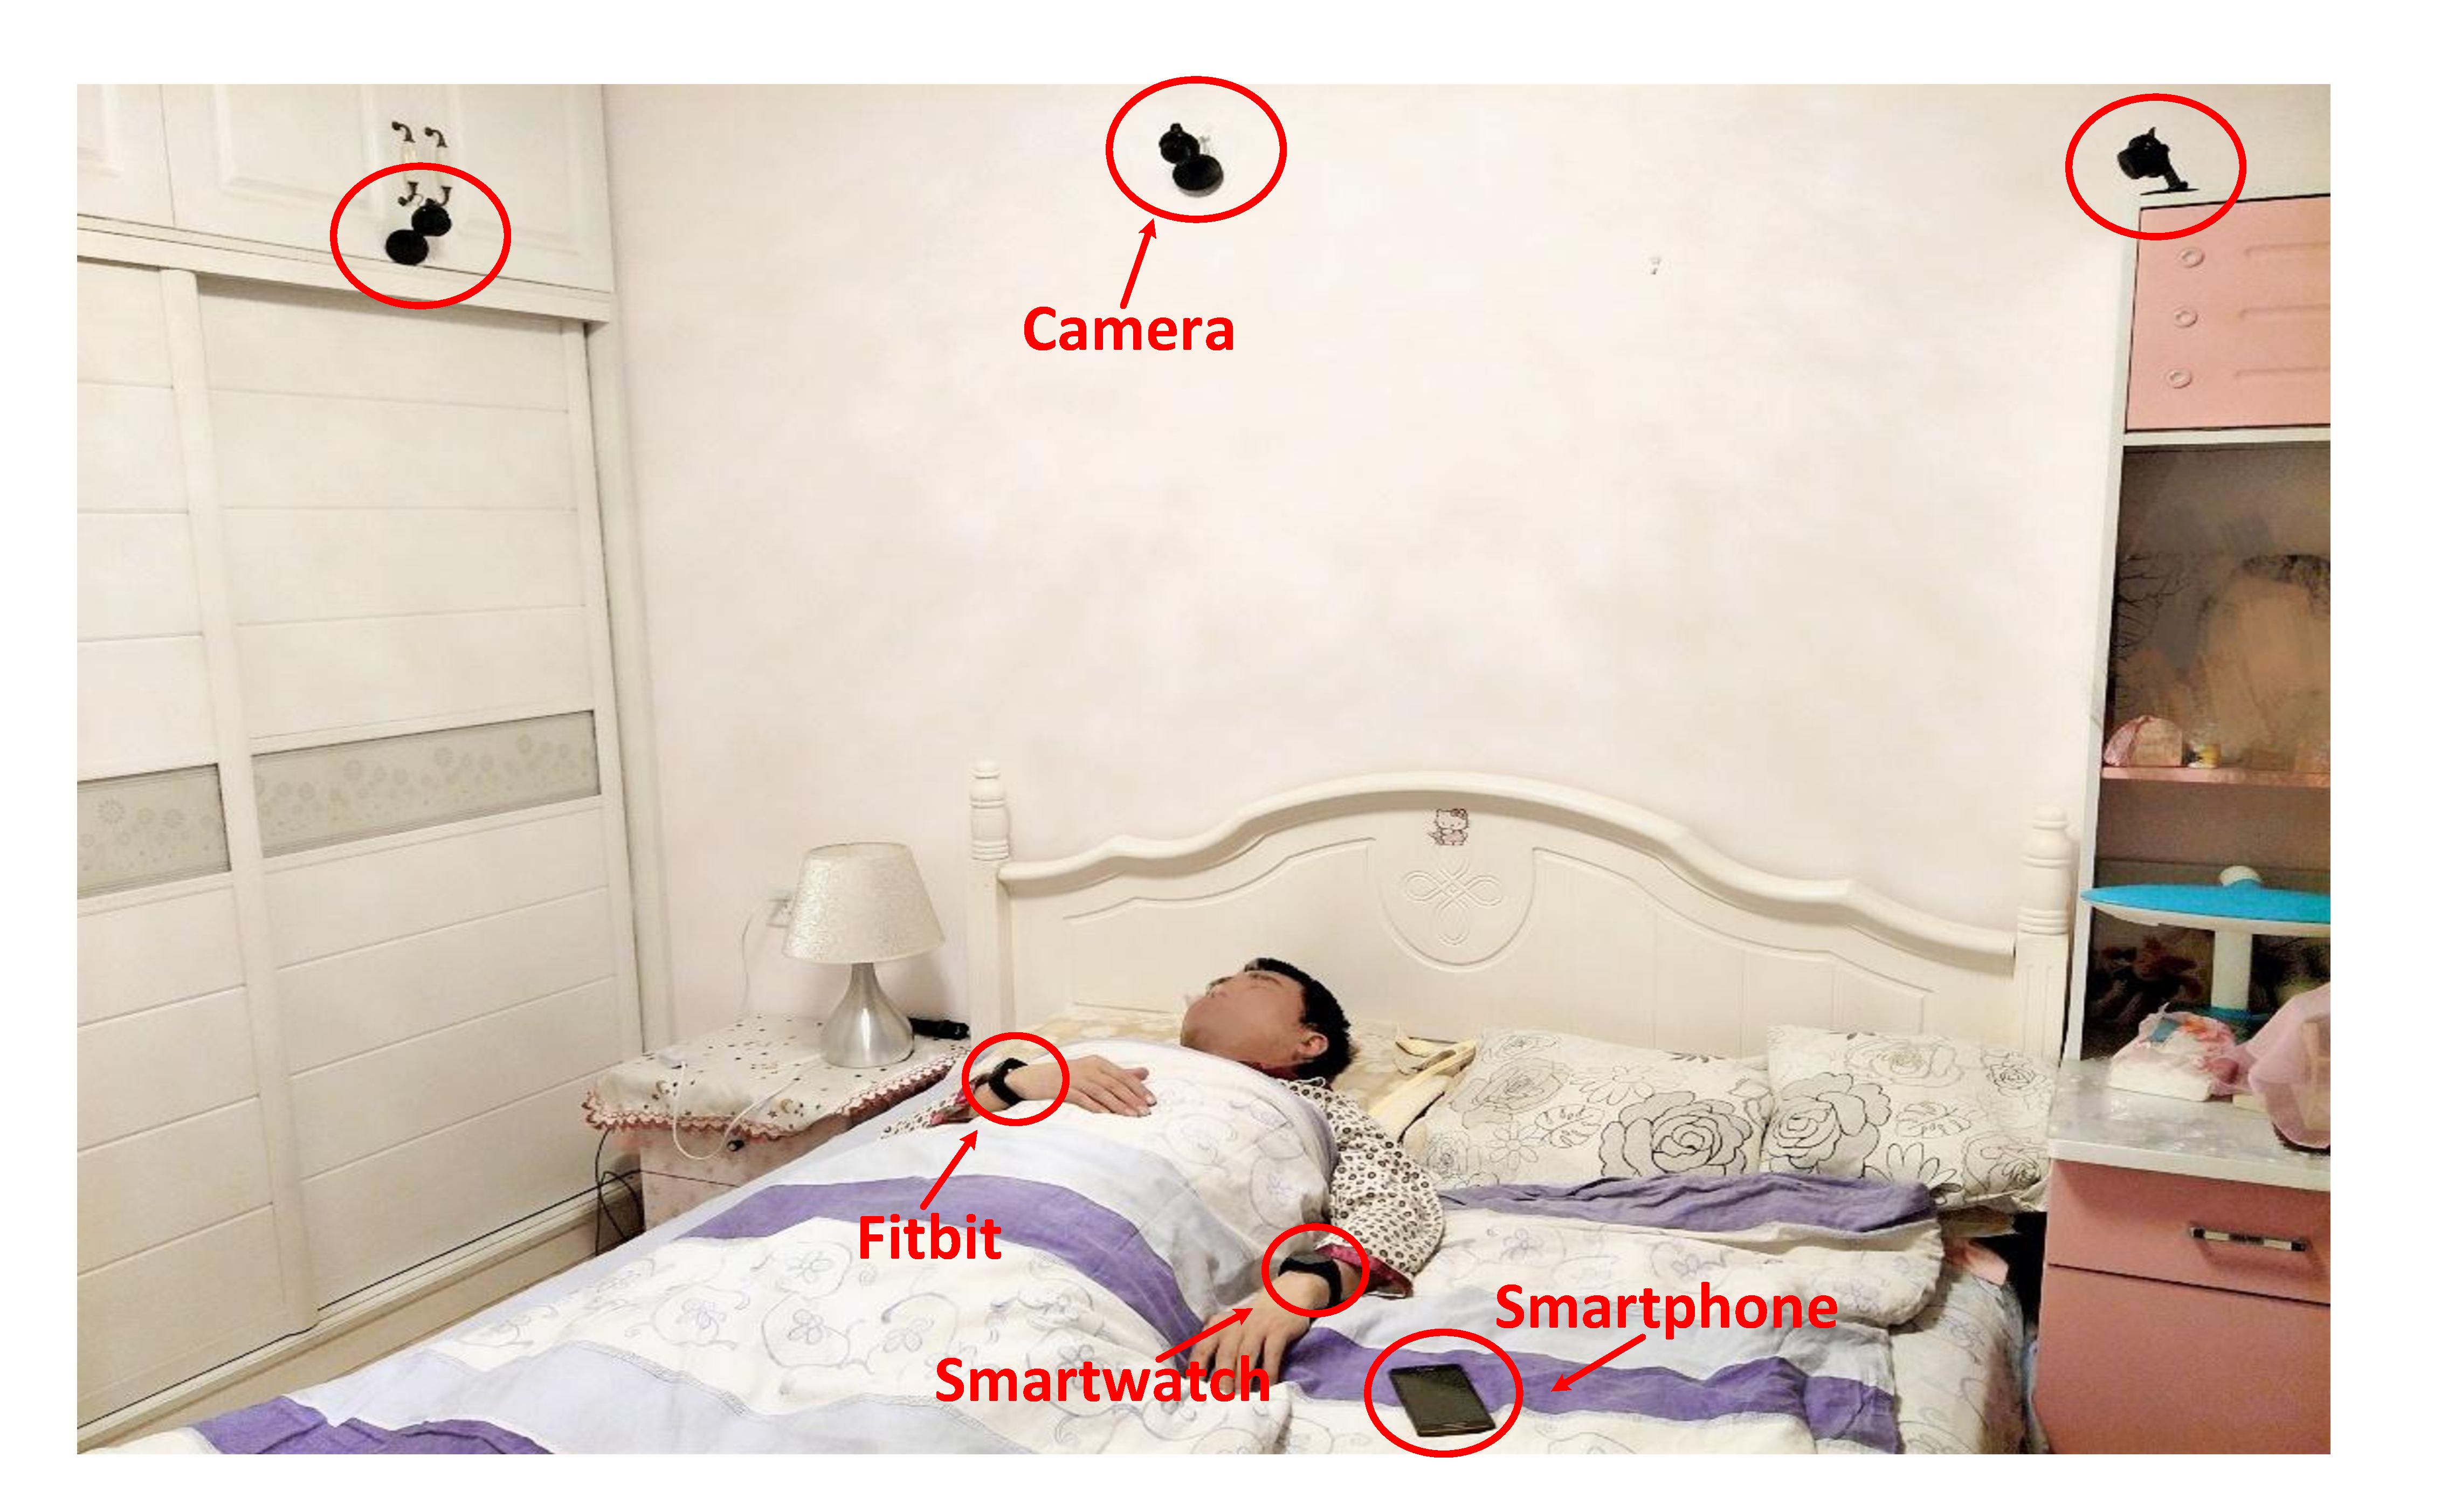
\includegraphics[width=0.52\linewidth]{Figures/setup.pdf}
	\caption{Deployment setup.}\label{fig:setup}
\end{figure}

\FIXME{ZW: here we should detail our experimental setup e.g. the environmental settings, how do we recruit the users, the mixture of the
users, what are the competitive models that we compare with, how do we report data (e.g. do we apply any statistical methods to remove the
outliers?), etc.}

\section{EXPERIMENTAL RESULTS}\label{sec:4experiment}
In this section, we detail the evaluation results for our system.

\subsection{Evaluation Results}
We focus on the detection accuracy about five events, that are body posture, the body rollover, the hand position, the micro body movement and the acoustic events.
%, the classification of micro body movement

\subsubsection{Performance of body posture classification}
We test the overall classification performance of different body postures. The groundtruth of body postures are recorded by the cameras. To simplify the experiment, we train the classifier using the data of only one user and then test the rest fourteen users, the accuracy is pretty good. Based on this, we use each user's data to train the classifier in turn. The averaged accuracy for 15 cases are the final performance, as shown in Fig. \ref{fig:posture_zhu}. We observe that the posture detection accuracy is consistently high across all users, and it does not show major variations across users. This good performance benifits from the distinct characteristics of arm position under different sleeping postures.

\begin{figure}[!t]
 \centering
 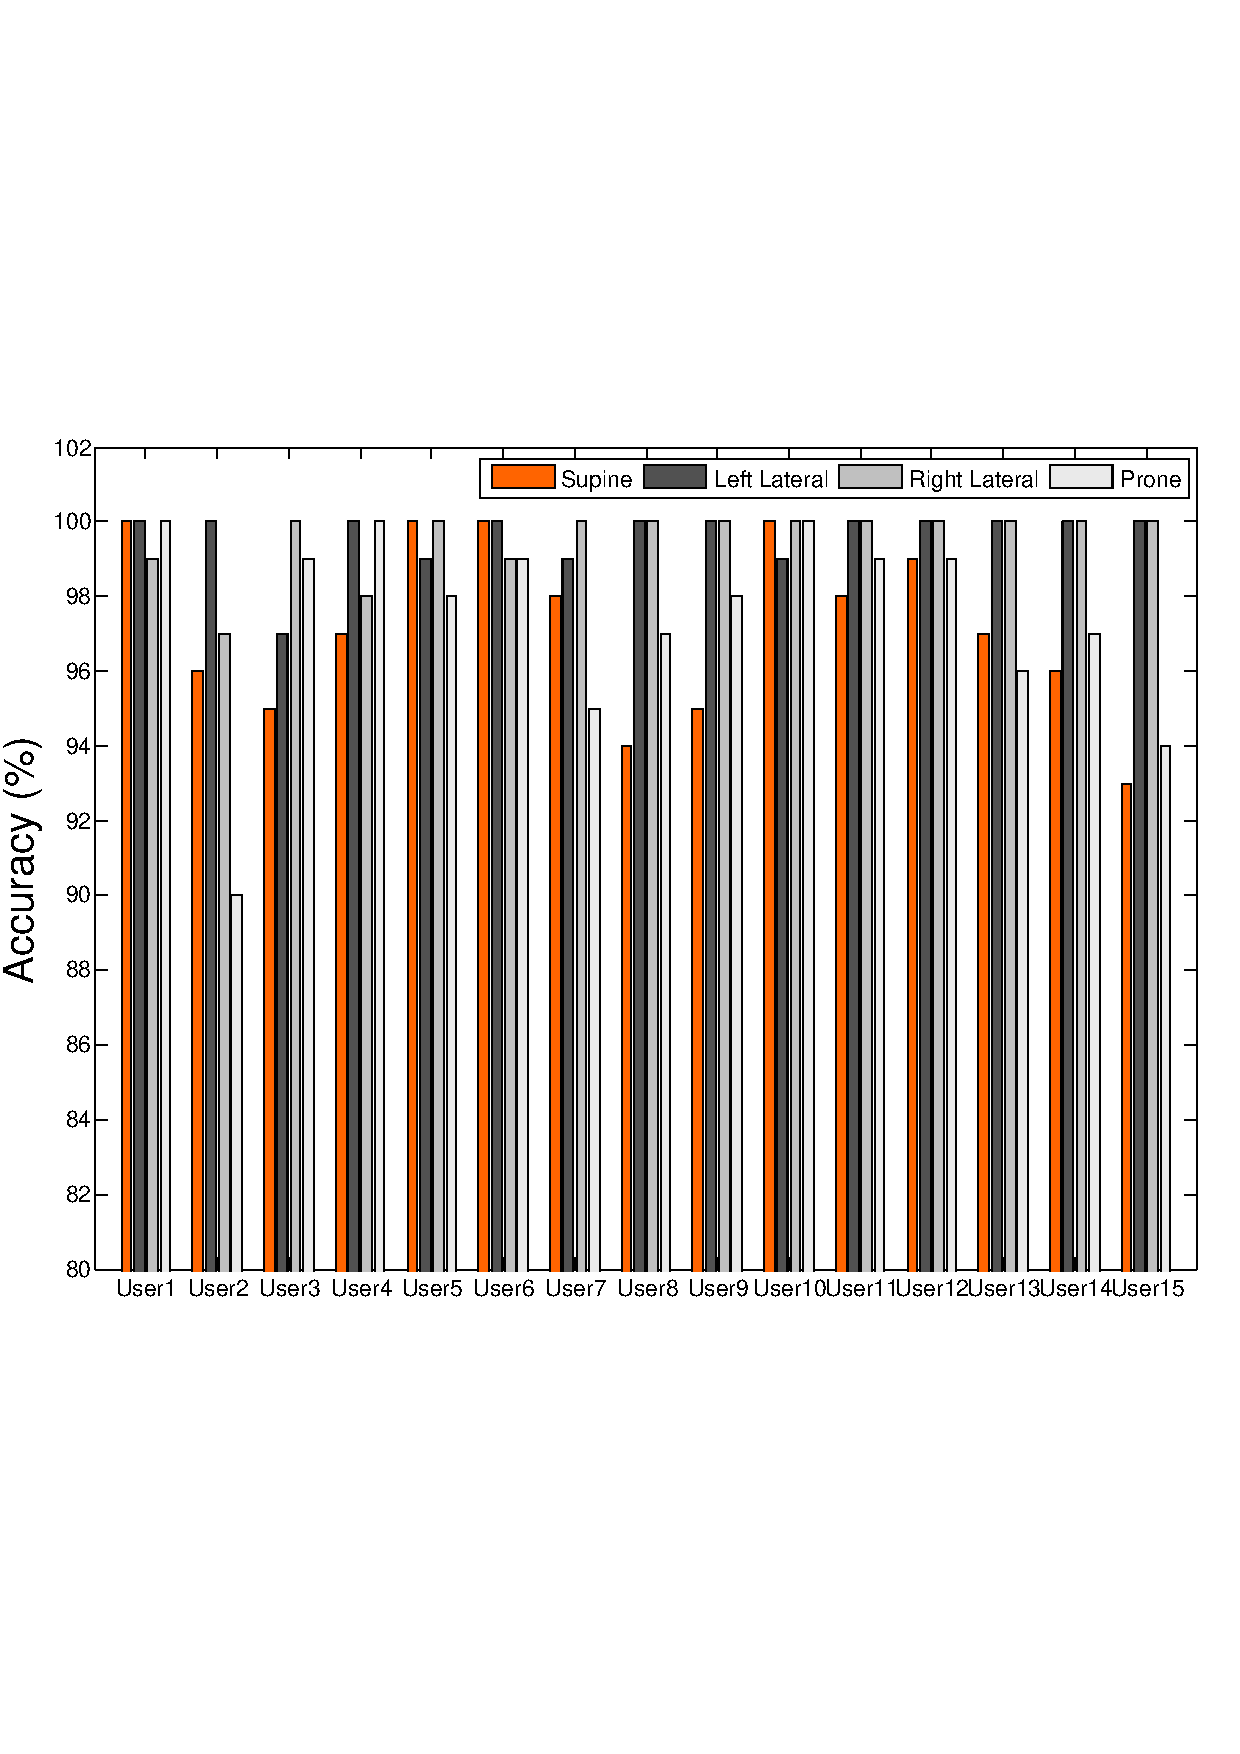
\includegraphics[width=0.52\linewidth]{Figures/posture_zhu.pdf}
 \caption{Detection accuracy of body postures.}\label{fig:posture_zhu}
 \end{figure}

\begin{table}[!thbp]
	\tabcolsep1pt
	\centering  % ������
	%\renewcommand\arraystretch{0.277}
	%\caption{The confusion matrix of body posture classification.}\label{tab:posture}
	%\noindent\makebox{%
	%\begin{tabular}{1\textwidth}{ c | c | c | c | c | c | c}
	\renewcommand\arraystretch{0.3}
	\caption{The confusion matrix of body posture classification.}\label{tab:posture}
	\begin{tabular}{c| c | c | c | c | c | c}
		\cline{1-7}
		&\multicolumn{1}{ c|}{ }
		& \multicolumn{4}{ c|}{ }\\
		\multirow{2}*{}
		&\multicolumn{1}{c|}{\multirow{2}*{{Result}}}
		&\multicolumn{4}{c|}{{Prediction}}
		& \multirow{4}*{{Recall}} \\
		%&\multicolumn{5}{ c |}{\textbf{\small Prediction}} \\
		% & \multicolumn{5}{ c |}{ } \\
		\cline{3-6}
		& & & & & \\
		\multicolumn{1}{c|}{{}}
		&  \multicolumn{1}{c|}{{}}
		&  \multicolumn{1}{c|}{{Supine}}
		&  \multicolumn{1}{c|}{{Left Lateral}}
		&  \multicolumn{1}{c|}{{Right Lateral}}
		&  \multicolumn{1}{c|}{{Prone}}   \\
		& & & & & \\
		\cline{1-7}
		& & & & & \\
		\multirow{5}{*}{\begin{sideways}{{Groundtruth}}\end{sideways}}
		&   {Supine}   & {\bf{{1182}}}    &   $25$      &   $4$      &   $9$    &   {96.7\%}\\
		& & & & & \\
		\cline{2-7}
		& & & & & \\
		&   {Left Lateral}   &   $6$      &   {\bf{{1292}}}     &   $0$      &   $0$   &   {99.5\%} \\
		& & & & & \\
		\cline{2-7}
		& & & & & \\
		&   {Right Lateral}   &   $7$      &   $0$      &  {\bf{{1275}}}      &   $12$  &   {98.5\%}  \\
		& & & & & \\
		\cline{2-7}
		& & & & & \\
		&   {Prone}   &   $19$      &   $2$      &   $3$      &   {\bf{{567}}}   &   {95.9\%} \\
		& & & & & \\
		\cline{1-7}
		& & & & & \\
		&   {Precision}    &   {97.3 \%}   &   {98.0\%}   &   {99.5\%}   &   {96.4\%}    \\
		& & & & & \\
		\cline{1-7}
	\end{tabular}
\end{table}

To have a deep evaluation about the sleep posture detection, we randomly choose one user to train the classifier. Then we calculate the detection precision and recall across postures. The result is shown in Table \ref{tab:posture}. The values in blocks are the corresponding numbers of four sleep postures from 14 test users. Due to that the angle features of acceleration are similar between the suspine posture with hand putting on the head and the left-lateral posture, a small amount of the supine postures are classified as left lateral.  The total amount of the prone posture is less than the number of other postures. It suggests that most people are not accustomed to sleep in the prone posture, because it is neither healthy nor comfortable. In coclude, Table \ref{tab:posture} shows the outstanding detection performance.



\subsubsection{Performance of body rollover counting}
To verify the efficiency of body rollover detection algorithm, we compare each user's  body rollover number detected by {\systemname} with the groundtruth recorded by camera. The performance is showed in Table \ref{tab:rollver}. We can see that User 3, User 4 and User 13 has an unusually high number, this difficulty in fall asleep results from the sleep disorder. For 15 users, the detection accuracies are all very high, and the least one is still 87\%. Thus {\systemname} can accurately distinguish the large hand movement from the body rollover in bed. However, detecting errors in body rollover events will not have a significant impact on our end result, because the division of the sleep stage is a comprehensive consideration of all the features of the sleep stage, such as micro body movement and acoustic events.

\begin{table}[!thbp]
  %\centering  % ������
  \tabcolsep 1pt
  %\arrayrulewidth1pt
  \caption{Detection accuracy of body rollover.}\label{tab:rollver}
   \renewcommand\arraystretch{1.3}{\multirowsetup}{\centering}
        \begin{tabular}{cccccccccccccccc}
        \toprule
         \textbf{User}    & 1& 2  & 3& 4& 5& 6& 7& 8& 9& 10& 11& 12& 13& 14& 15\\
        \midrule
         \rowcolor{Gray}      { Groundtruth}  &231&204&442&397&198&101&196&164&193&208&131&205&342&149&156 \\
                 { Accuracy} &91\%& 94\% &88\%&93\%&96\%&94\%&87\%&90\% &93\% &94\% &92\% &94\% &89\% &90\% &95\%\\
        \bottomrule
 \end{tabular}
\end{table}

\subsubsection{Performance of hand position recognition}
\textcolor{blue}{To test the identification performance of different hand positions, {\systemname} uses a cross-validation approach that uses only one user's data at a time to train the classifier, and the remaining 14 users' data are treated as test data sets.} The classifier for detecting the hand movement trajectory is combined with the detection of periodic signals caused by respiration, then the hand position which is on the chest or abdomen or head can be identified. Fig. \ref{fig:hand_zhu} illustrates the accuracy of hand position across 15 people. As we can see that with just one set of training data, the accuracies for different users are all higher than 87\%. Therefore, our system can achieve a satisfied identification accuracy for different hand positions at a small price. Moreover, we found that at least four persons out of fifteen participants would tend to put their hands on their heads when they sleep in the supine, which is a bad habit for sleep. And other participants' hand are also often placed at these positions of our interest when they are in their supine posture.


\begin{figure}
 \centering
 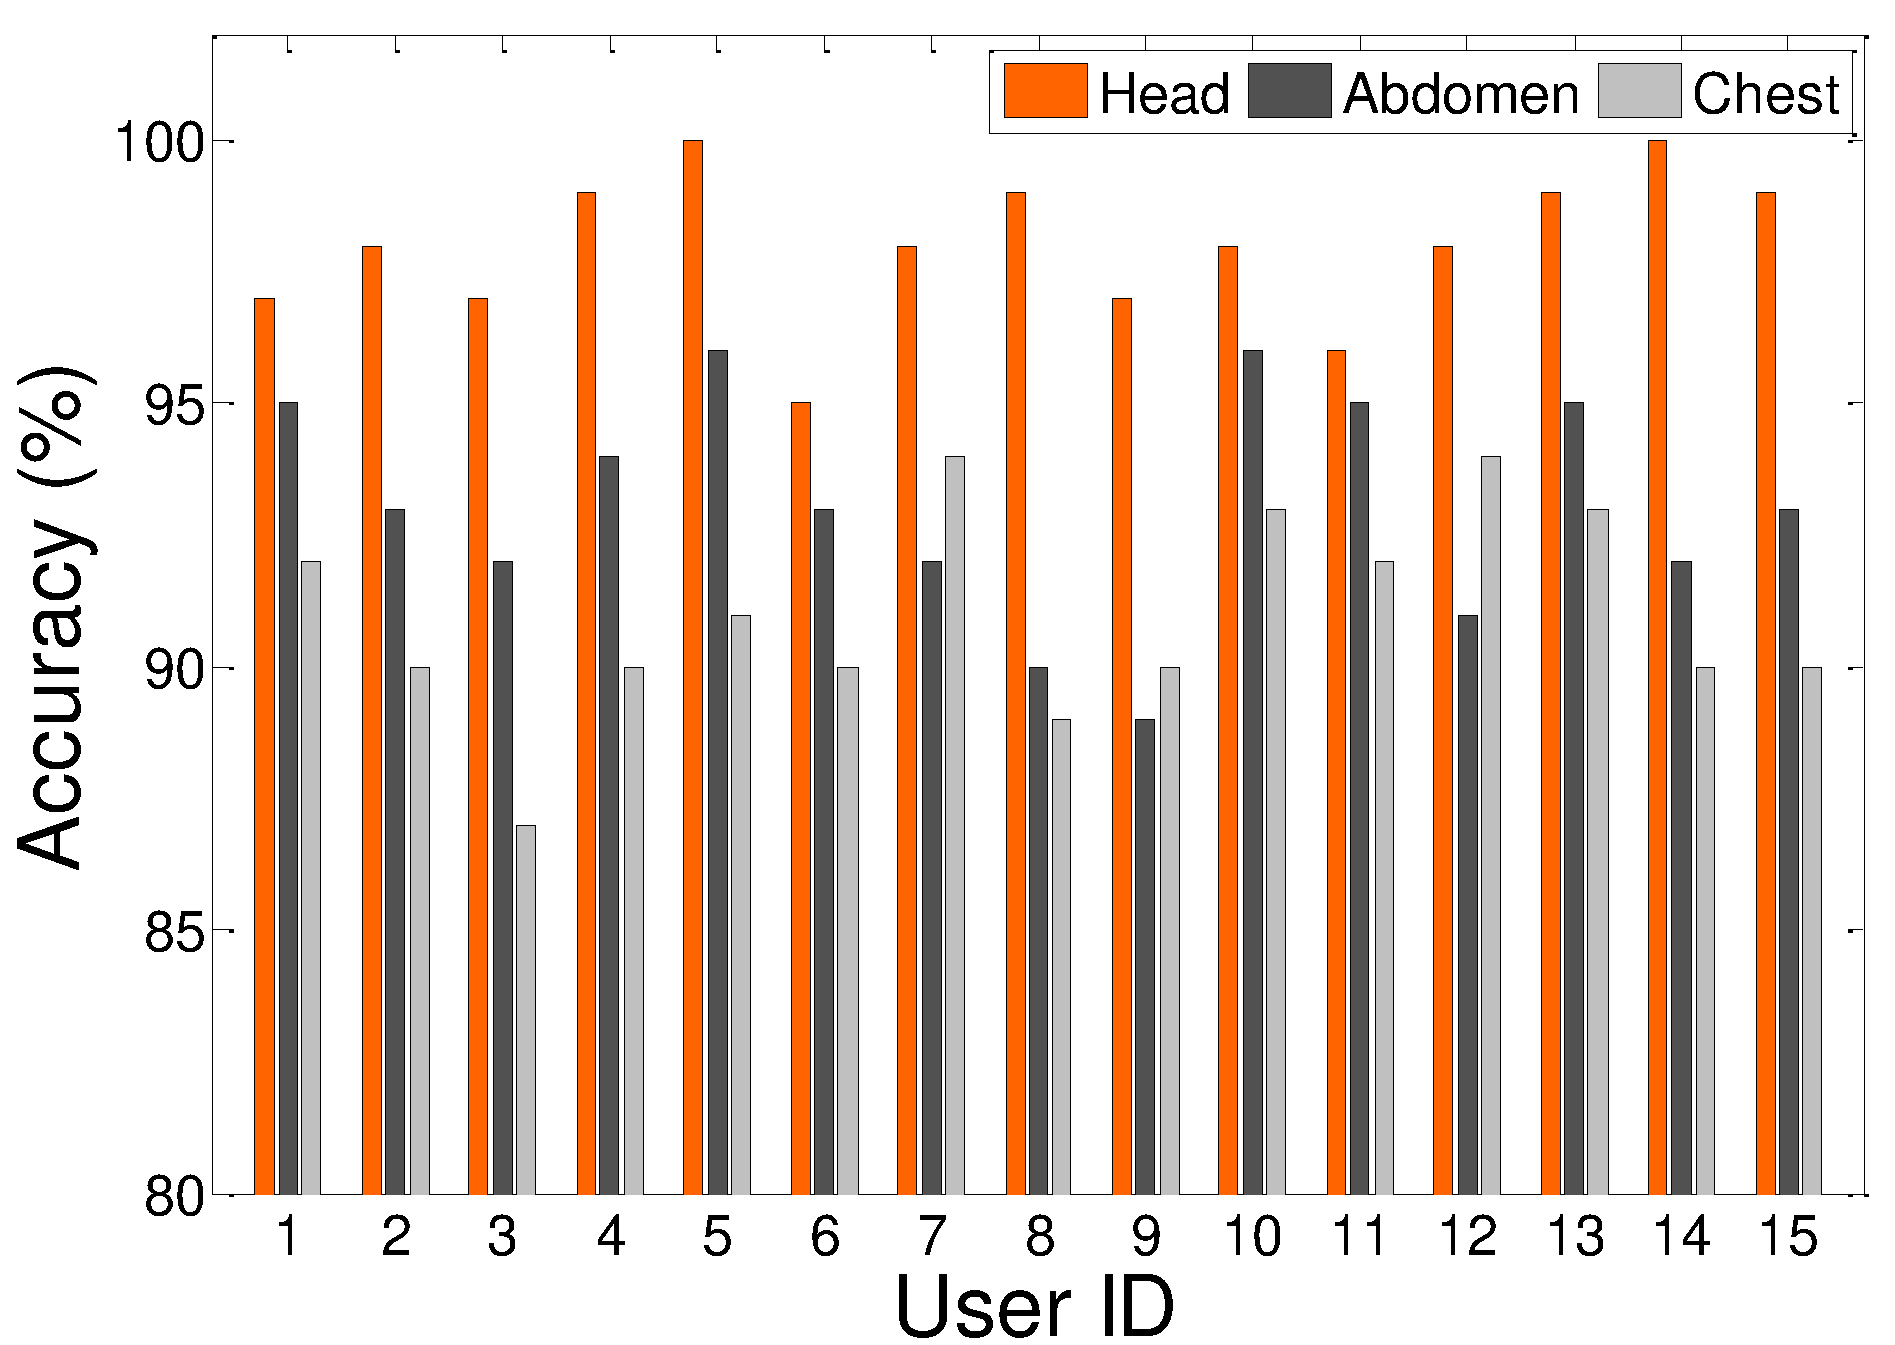
\includegraphics[width=0.52\columnwidth]{Figures/handposition_zhu.pdf}
 \caption{Identification accuracy of hand positions}\label{fig:hand_zhu}
\end{figure}




\subsubsection{Performance of micro body movement detection}
To assess the performance of {\systemname}'s detection and classification of user's micro body movements during sleep, we manually mark the types of the micro body movements (hand moving, arm raising, and body trembling) recorded by the camera that occur during sleep. At the same time, we use the accelerometer embedded in a smartphone placed on the bed to record the occurrence of the micro body movements, so as to avoid some movements such as trembling of the body being ignored due to being covered by coverings (such as quilts). And then we combine the two to serve as groundtruth. Fig. \ref{fig:micro_movement_zhu} illustrates the accuracy of the body micro-motion classification across 15 people. We observed that the micro-motion detection accuracy of all users is very close, that is, there will be no major changes between users. And from Fig. \ref{fig:micro_combine}, we can see that even though the worst classification result belongs to the hand movement, the average precision and recall rate still exceed 75\%, and the average accuracy of arm raising and body trembling are 93 \%, 84\%, which indicates that the accuracy of the classification is acceptable. And our purpose of detecting micro body movement is to help us detect the sleep stage, so we are more concerned with body trembling and arm raising, and the poor accuracy of hand moving does not have a significant impact on our end result. The reason for the poor performance of hand movement and body trembling classification may be that we have fewer people to refer to when setting the threshold of the peak value. Specifically, we can further consider more different people in different situations, or set their own thresholds for each person by observing or learning each person's sleep data.


\begin{figure}
\setlength{\abovecaptionskip}{0.cm}
\setlength{\belowcaptionskip}{-0.cm}
 \centering
 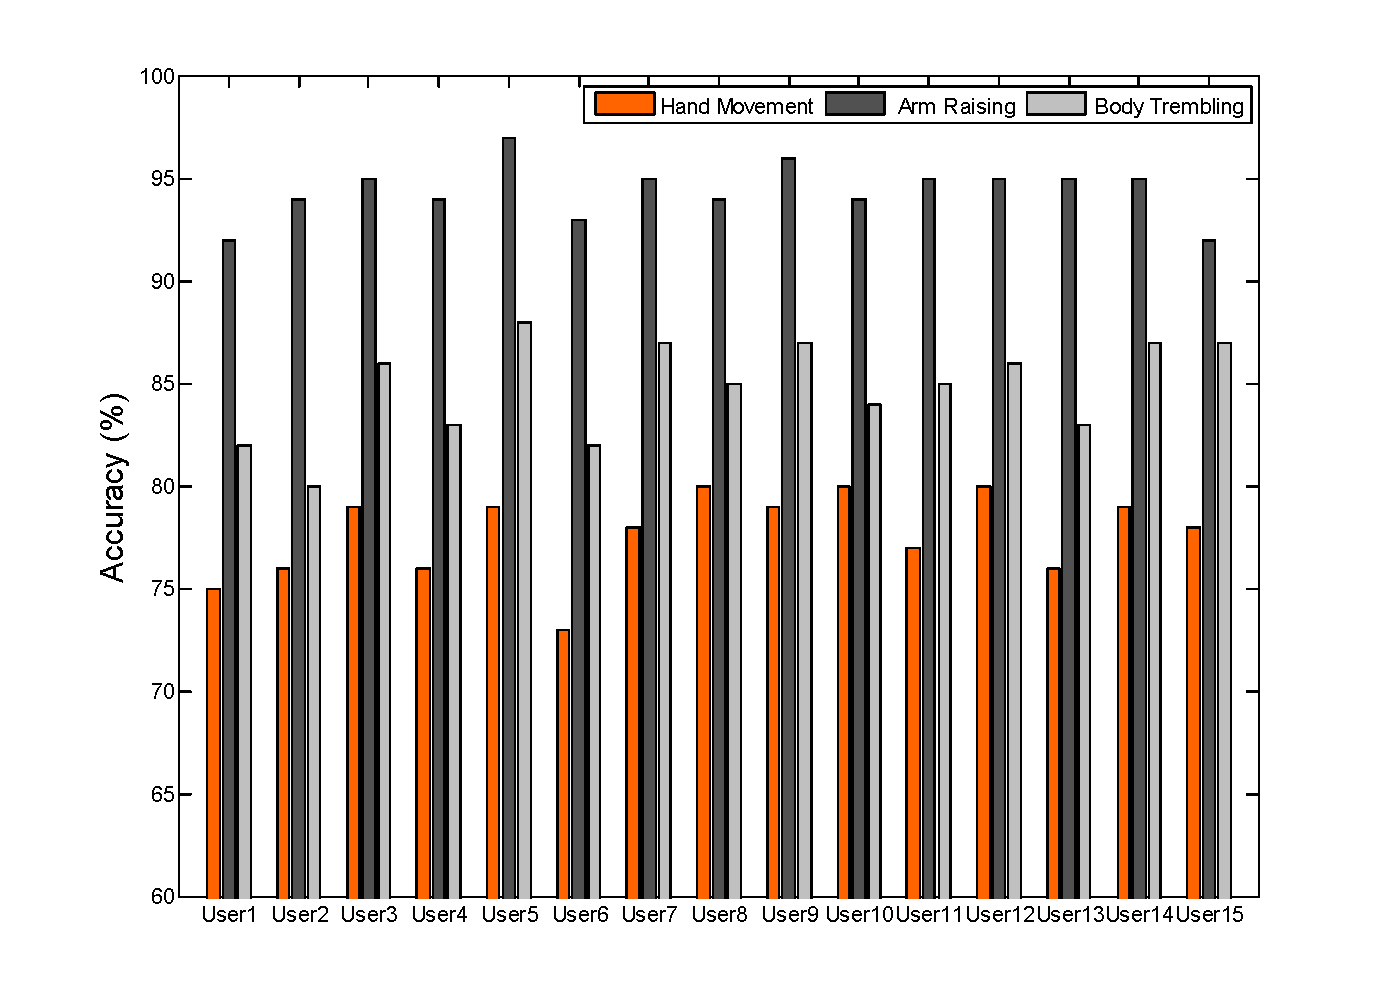
\includegraphics[width=0.52\linewidth]{Figures/micro_movement_zhu.pdf}
 \caption{Detection accuracy of micro body movement.}\label{fig:micro_movement_zhu}
\end{figure}

\begin{figure}
 \centering
   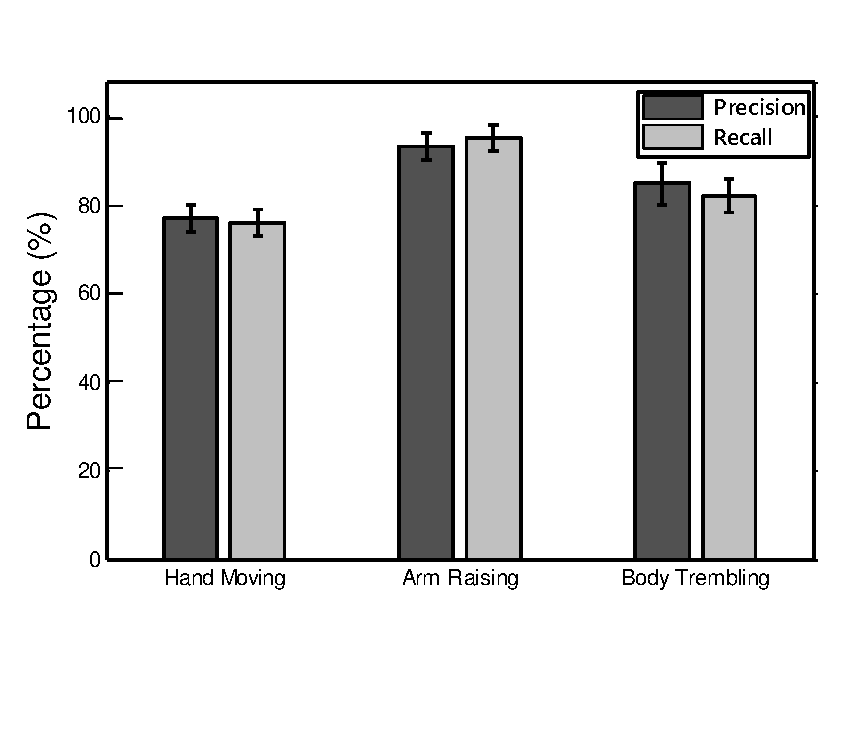
\includegraphics[width=0.52\linewidth]{Figures/micro_combine1.pdf}
 \caption{Micro body movement}\label{fig:micro_combine}
\end{figure}



 \subsubsection{Performance of acoustic events detection}
To study the detection accuracies of different acoustic events, we compare the groundtruth recorded by the camera with the detected results by our system. Table \ref{tab:sound} shows the results across 15 test participants. We can see that the accuracy for cough event is 88.9\%, which is relative lower with regard to other three events. The reason is that different user's cough pattern are different, the pre-defined parameters used in the system does not include all possible patterns. When we train the parameters of the detection algorithm, we only collect 120 sets of nighttime sound data. The data come from 40 (21 males and 19 females) volunteers of different ages (ages 15 to 60) who are prone to snoring, coughing, or somniloquy at night. So in order to further improve the detection accuracy, we can train particular parameters for more different users.

\begin{table}[!thbp]
 \tabcolsep1pt
  \centering  % ������
  \renewcommand\arraystretch{0.3}
  \caption{The confusion matrix of acoustic events detection.}\label{tab:sound}
\begin{tabular}{c| c | c | c | c | c | c}
   \hline
   &\multicolumn{1}{ c|}{ }
   & \multicolumn{4}{ c|}{ }\\
   \multirow{2}*{}
&\multicolumn{1}{c|}{\multirow{2}*{{ Result}}}
&\multicolumn{4}{c|}{{ Prediction}}
& \multirow{4}*{{ Recall}} \\
    %&\multicolumn{5}{ c |}{\textbf{\small Prediction}} \\
   % & \multicolumn{5}{ c |}{ } \\
    \cline{3-6}
    & & & & & \\
    \multicolumn{1}{c|}{{}}
    &  \multicolumn{1}{c|}{{}}
    &  \multicolumn{1}{c|}{{ Snore}}
    &  \multicolumn{1}{c|}{{ Cough}}
    &  \multicolumn{1}{c|}{{ Somniloquy}}
    &  \multicolumn{1}{c|}{{ Other}}   \\
    & & & & & \\
     \cline{1-7}
    & & & & & \\
    \multirow{5}{*}{\begin{sideways}{{ Groundtruth}}\end{sideways}}
    &   { Snore}   & {\bf{{96}}}    &   $0$      &   $0$      &   $9$    &   {91.4\%}\\
    & & & & & \\
    \cline{2-7}
    & & & & & \\
   &   { Cough}   &   $3$      &   {\bf{{64}}}     &   $0$      &   $4$   &   {90.1\%} \\
    & & & & & \\
     \cline{2-7}
    & & & & & \\
    &   { Somniloquy}   &   $0$      &   $3$      &  {\bf{{42}}}      &   $2$  &   {89.4\%}  \\
    & & & & & \\
     \cline{2-7}
    & & & & & \\
    &   { Other}   &   $0$      &   $5$      &   $4$      &   {\bf{{325}}}   &   {97.3\%} \\
    & & & & & \\
    \hline
    & & & & & \\
    &   { Precision}      &   {96.9\%}   &   {88.9\%}   &   {91.3\%}   &   {95.6\%}    \\
    & & & & & \\
    \hline
   \end{tabular}
\end{table}


\subsection{Overall performance}

\subsubsection{Performance of sleep stage detection}
In order to prove that the detected events not only reflect the user's sleep habits, but also effectively divide the sleep stage in order to assess the quality of sleep, we regard the reported results from Fitbit Charge2 as the ground truth.  \textcolor{blue}{We randomly selected 50 sets of nocturnal sleep data from 210 sets of sleep data collected from 15 participants for 2 weeks as the test data, what's more, we need to make sure that no less than 3 sets of nocturnal sleep data in these test data come from the same participant. It is worth mentioning that, {\ systemname} bases on the event detected by each submodule every 5 minutes to determine the sleep stage.} The average values of precision and recall are shown in Table \ref{tab:sleep stage}. From this table, we can see that although {\systemname} may often make misjudgement between light sleep stage and REM, the overall detection performance of {\systemname} is satisfying.

\begin{table}[!thbp]
 \tabcolsep1pt
  \centering  % ������
  \renewcommand\arraystretch{0.4}
  \caption{\textcolor{blue}{Performance of sleep stage detection.}}\label{tab:sleep stage}
\begin{tabular}{c| c | c | c | c | c}
   \hline
   &\multicolumn{1}{ c|}{ }
   & \multicolumn{3}{ c|}{ }\\
   \multirow{2}*{}
&\multicolumn{1}{c|}{\multirow{2}*{{ Result}}}
&\multicolumn{3}{c|}{{ Prediction}}
& \multirow{3}*{{ Recall}} \\
    %&\multicolumn{5}{ c |}{\textbf{\small Prediction}} \\
   % & \multicolumn{5}{ c |}{ } \\
    \cline{3-5}
    & & & & & \\
    \multicolumn{1}{c|}{{}}
    &  \multicolumn{1}{c|}{{}}
    &  \multicolumn{1}{c|}{{ REM}}
    &  \multicolumn{1}{c|}{{ Light Sleep}}
    &  \multicolumn{1}{c|}{{ Deep Sleep}} \\
    & & & & & \\
     \cline{1-6}
    & & & & & \\
    \multirow{4}{*}{\begin{sideways}{{ Groundtruth}}\end{sideways}}
    &   { REM}   & {\bf{{986}}}    &   $337$      &   $84$     &   {70.0\%}\\
    & & & & & \\
     & & & & & \\
    \cline{2-6}
    & & & & & \\
   &   { Light Sleep}   &   $319$      &   {\bf{{1007}}}     &   $120$      &   {69.6\%} \\
    & & & & & \\
     \cline{2-6}
    & & & & & \\
    &   { Deep Sleep}   &   $83$      &   $171$      &  {\bf{{378}}}      &   {59.8\%}  \\
    & & & & & \\
     \cline{1-6}
     & & & & & \\
    &   { Precision}      &   {71.0\%}   &   {66.5\%}   &   {64.9\%}   \\
    & & & & & \\
    \hline
   \end{tabular}
\end{table}

\subsubsection{Evaluation on the effect of respiratory amplitude on sleep stage detection}
When we detect the hand's position in the abdomen or chest, we use the magnitude of the acceleration to estimate the amplitude of the respiration. To assess the effectiveness of {\systemname}'s detection of respiration amplitude, we evaluated the performance of the sleep stage test separately in two cases that with considering respiration amplitude and without considering respiration amplitude. And then we can measure the contributions of it for classification of the sleep stage, as we can see in Table \ref{tab:respiratory}. Obviously, When we consider the division of the sleep stage, combining breathing amplitude as a feature with other features, we find that the precision and recall of each sleep stage improve, which proves the effectiveness of our detection of respiration amplitude.

\begin{table} \footnotesize
  \centering  % ������
  \renewcommand\arraystretch{0.3}
  \caption{\textcolor{blue}{Evaluation of respiration amplitude contribution}}\label{tab:respiratory}
\begin{tabular}{c| c | c | c | c | c | c| c |}
   \cline{2-8}
   &\multicolumn{1}{ c|}{ }
   &\multicolumn{2}{ c|}{ }
   &\multicolumn{2}{ c|}{ }
   & \multicolumn{2}{ c|}{ }\\
   %  \multirow{4}*{}
    &\multicolumn{1}{c|}{}
   &\multicolumn{2}{c|}{\textbf{\scriptsize REM}}
   &\multicolumn{2}{c|}{\textbf{\scriptsize Light Sleep}}
   &\multicolumn{2}{c|}{\textbf{\scriptsize Deep Sleep}} \\
    %&\multicolumn{5}{ c |}{\textbf{\small Prediction}} \\
   % & \multicolumn{5}{ c |}{ } \\
    \cline{2-8}
    & & & & & & &\\
    \multicolumn{1}{c|}{\textbf{}}
    &  \multicolumn{1}{c|}{\textbf{Features}}
    &  \multicolumn{1}{c|}{\scriptsize Precision}
    &  \multicolumn{1}{c|}{\scriptsize Recall}
    &  \multicolumn{1}{c|}{\scriptsize Precision}
    &  \multicolumn{1}{c|}{\scriptsize Recall}
    &  \multicolumn{1}{c|}{\scriptsize Precision}
    &  \multicolumn{1}{c|}{\scriptsize Recall}\\
    & & & & & & &\\
     \cline{2-8}
    & & & & & & &\\
    \multirow{5}{*}
    &   \textbf{\scriptsize Without Respiration Amplitude}   & $62.9\%$    &   $63.4\%$      &   $59.4\%$      &   $63.9\%$    &   $58.7\%$ &  $54.1\%$ \\
    & & & & & & &\\
    \cline{2-8}
    & & & & & & &\\
   &   \textbf{\scriptsize With Respiration Amplitude}   &   $71.0\%$      &   $70.0\%$     &   $66.5\%$      &   $69.7\%$   &   $64.9\%$ &   $59.8\%$ \\
    & & & & & & &\\

   \cline{2-8}

   \end{tabular}
\end{table}

\subsubsection{Performance comparison}
To our knowledge, in the current actigraphy-based work, there is no clear baseline for sleep stage detection performance for us. So we
decided to compare {\systemname} with the sleep detection app, Sleep As Android, that has been widely used in the marketplace, in addition,
we also considered a comparison with Sleep Hunter \cite{gu2016sleep}. Table \ref{tab:comparison} shows the performance of the sleep stage
detection, Sleep As Android can only detect light sleep stage and the deep sleep stage, so we only compared the performance of these two
stages.

 \begin{table} \footnotesize
  \centering  % ������
  \renewcommand\arraystretch{0.3}
  \caption{\textcolor{blue}{Performance Comparison}}\label{tab:comparison}
\begin{tabular}{c| c | c | c | c | c |}
   \cline{2-6}
   &\multicolumn{1}{ c|}{ }
   &\multicolumn{2}{ c|}{ }
   &\multicolumn{2}{ c|}{ }\\
   %  \multirow{4}*{}
    &\multicolumn{1}{c|}{}
   &\multicolumn{2}{c|}{\textbf{\scriptsize Light Sleep}}
   &\multicolumn{2}{c|}{\textbf{\scriptsize Deep Sleep}} \\
    %&\multicolumn{5}{ c |}{\textbf{\small Prediction}} \\
   % & \multicolumn{5}{ c |}{ } \\
    \cline{2-6}
    \multicolumn{1}{c|}{\textbf{}}
    &  \multicolumn{1}{c|}{\diagbox{System}{Stage}}
    &  \multicolumn{1}{c|}{\scriptsize Precision}
    &  \multicolumn{1}{c|}{\scriptsize Recall}
    &  \multicolumn{1}{c|}{\scriptsize Precision}
    &  \multicolumn{1}{c|}{\scriptsize Recall}\\
     \cline{2-6}
    & & & & & \\
    \multirow{5}{*}
    &   \textbf{\scriptsize SleepGuard}   & $66.5\%$    &   $69.6\%$      &   $64.9\%$      &   $59.8$  \\
    & & & & &  \\
    \cline{2-6}
    & & & & & \\
   &   \textbf{\scriptsize Sleep As Android}   &   $27.8\%$      &   $35.4\%$     &   $35.7\%$      &   $50.2\%$   \\
    \cline{2-6}
    & & & & & \\
    &   \textbf{\scriptsize Sleep Hunter}   &   $66.74\%$      &   $66.11\%$     &   $60.00\%$      &   $50.73\%$   \\

   \cline{2-6}

   \end{tabular}
\end{table}

As we can see, {\systemname} can not only perform better on sleep stage detection than Sleep As Android, but also detect one more sleep stage. \textcolor{blue}{As for Sleep Hunter, our system's detection ability is slightly better than its. This may be because {\systemname} detects sleep-related events with better performance and incorporates respiratory amplitude considerations. And our system can provide richer sleep data for users and take more factors that affect sleep quality into consideration, making users understand their sleep more easily and improve their sleep quality more effectively.} Further, we show our superior in function comapared with other similar sleep detection products, including Sleep As Android, Sleep Hunter, sleepMonitor \cite{sleepmonitor}, Sleeptracker \cite{sleeptracker}, Fitbit, isleep \cite{hao2013isleep}, Jawbone \cite{Jawbone},ubiSleep \cite{pombo2016ubisleep}, in Table \ref{tab:function}. As we have shown, {\systemname} can detect a wider range of sleep events to provide a better user experience.

\begin{table*}\scriptsize
\setlength{\abovecaptionskip}{0.8pt}
  \centering  % ������
  \tabcolsep10pt
  \arrayrulewidth1pt
  \caption{Systems for support sleep}\label{tab:function}
  \renewcommand{\multirowsetup}{\centering}
  \noindent\makebox[\textwidth]{%
        \begin{tabularx}{1.0\textwidth}{|c|c|c|c|c|c|c|}
        \cline{1-7}
        \multicolumn{1}{|c|}{\multirow{2}*{\textbf{\scriptsize System}}}
        &\multicolumn{6}{c|}{\textbf{ \scriptsize Detected Events}} \\
         \cline{2-7}
    &  \multicolumn{1}{c|}{\textbf{ \scriptsize Heart Rate }}
    &  \multicolumn{1}{c|}{\textbf{ \scriptsize Acoustic Event }}
    &  \multicolumn{1}{c|}{\textbf{ \scriptsize Sleep Posture }}
     &  \multicolumn{1}{c|}{\textbf{ \scriptsize body Movement }}
      &  \multicolumn{1}{c|}{\textbf{ \scriptsize hand position}}
       &  \multicolumn{1}{c|}{\textbf{ \scriptsize Sleep Stage}} \\
        \cline{1-7}
        \multirow{7}{2cm}
        {\textbf{SleepGuard\\Sleep as Android\\Sleep Hunter\\SleepMonitor\\Sleeptracker\\isleep \\Fitbit\\Jawbone\\ ubiSleep } }
        & &$\checkmark$ & $\checkmark$ &  $\checkmark$  &$\checkmark$ &$\checkmark$\\
        & &$\checkmark$ & & & &$\checkmark$\\
        & & $\checkmark$& &$\checkmark$ & &$\checkmark$\\
        & & & $\checkmark$ & & &\\
        &$\checkmark$ & & & & &$\checkmark$\\
         & &$\checkmark$ &   &$\checkmark$ & &\\
         &$\checkmark$ & & & & &$\checkmark$ \\
        & & & & & &$\checkmark$ \\
        & $\checkmark$&$\checkmark$ & & & &\\
        \cline{1-7}
 \end{tabularx}}
\end{table*}

\subsubsection{User survey}
In order to evaluate whether {\systemname} can provide help in the assessment of sleep quality and has a good user experience, we conducted a user survey of 15 volunteers participating in our experiments. In our survey, we asked participants to fill out our questionnaire based on PSQI \cite{carpenter1998psychometric} every morning during the experiment, in order to get their subjective feeling of sleep quality and use experience for our system. We use the following questions in our survey, which includes:
\begin{enumerate}
  \item Subjective sleep quality (5 levels, 1 for excellent and 5 for worst)
  \item Sleep duration
  \item Sleep disturbances
  \item Daytime dysfunction
\end{enumerate}

\textcolor{blue}{The average 14-day sleep quality score for 15 individuals are shown in Table. \ref{tab:quality}, we have listed three kinds of sleep quality assessment mechanims, namely, {\systemname}, Fitbit and user survey, where the sleep quality score obtained by user survey comes from the comprehensive scores of the questionnaires based on the above aspects. For the above four items, each one is rated on a 1-5 scale. These component scores are then summed to yield a score, which has a range of 0-20. And we divide each five scores into one and eventually divide the total score into four levels, recorded as 0-3, representing poor, general, good and excellent respectively, that is higher scores indicate better sleep quality. From the table, we can see the result is satisfactory and representative to some extent.} In addition, we also ask whether users are interested in these events, such as sleep posture, hand position, which detected by {\systemname}. 80\% of participants believe that the detection of sleep posture is very necessary, showing their sleep posture can not only help people to avoid health problems caused by long-term improper sleeping posture, but also help us find out the reasons for the next day's physical discomfort, such as dizziness, muscle soreness may be due to improper sleeping position. 60\% of the participants thought it useful to detect their hand position in the supine position and even one user mentioned that he did often have nightmares and that he found his hands were often placed on his chest. And {\systemname} was able to remind him to avoid such a hand position when sleeping. However, only 20\% of them think it is necessary to calculate the number of body rollover, but the detection of body rollover is very useful in the division of sleep stage.


\begin{table} \footnotesize
  \centering  % ������
  \renewcommand\arraystretch{0.3}
  \caption{\textcolor{blue}{Results of sleep quality assessment}}\label{tab:quality}
\begin{tabular}{c| c | c | c | c | c |c |c |c |c |c| c |c |c |c |c |c |c|}
   %\cline{2-6}
   %&\multicolumn{1}{ c|}{ }
   %&\multicolumn{2}{ c|}{ }
  % &\multicolumn{2}{ c|}{ }\
    %&\multicolumn{1}{c|}{}
   %&\multicolumn{2}{c|}{\textbf{\scriptsize Light Sleep}}
  % &\multicolumn{2}{c|}{\textbf{\scriptsize Deep Sleep}} \\
    %&\multicolumn{5}{ c |}{\textbf{\small Prediction}} \\
   % & \multicolumn{5}{ c |}{ } \\
    \cline{2-17}
    \multicolumn{1}{c|}{\textbf{}}
    &  \multicolumn{1}{c|}{\diagbox{System}{User}}
    &  \multicolumn{1}{c|}{\scriptsize User 1}
    &  \multicolumn{1}{c|}{\scriptsize User 2}
    &  \multicolumn{1}{c|}{\scriptsize User 3}
    &  \multicolumn{1}{c|}{\scriptsize User 4}
    &  \multicolumn{1}{c|}{\scriptsize User 5}
    &  \multicolumn{1}{c|}{\scriptsize User 6}
    &  \multicolumn{1}{c|}{\scriptsize User 7}
    &  \multicolumn{1}{c|}{\scriptsize User 8}
    &  \multicolumn{1}{c|}{\scriptsize User 9}
    &  \multicolumn{1}{c|}{\scriptsize User 10}
    &  \multicolumn{1}{c|}{\scriptsize User 11}
    &  \multicolumn{1}{c|}{\scriptsize User 12}
    &  \multicolumn{1}{c|}{\scriptsize User 13}
    &  \multicolumn{1}{c|}{\scriptsize User 14}
    &  \multicolumn{1}{c|}{\scriptsize User 15}\\
     \cline{2-17}
    & & & & & & & & & & & & & & & & \\
    \multirow{16}{*}
    &   \textbf{\scriptsize SleepGuard}  & $3$ & $3$ & $0$ & $2$ & $2$ & $1$ & $3$ & $0$ & $2$ & $2$ & $2$ & $2$ & $1$ & $0$ & $2$ \\
   & & & & & & & & & & & & & & & &\\
    \cline{2-17}
   & & & & & & & & & & & & & & & &\\
   &   \textbf{\scriptsize Fitbit}   & $3$ & $3$ & $0$ & $3$ & $1$ & $0$ & $2$ & $3$ & $2$ & $2$ & $2$ & $2$ & $2$ & $1$ & $2$\\
    \cline{2-17}
    & & & & & & & & & & & & & & & & \\
    &   \textbf{\scriptsize User survey}  & $3$ & $2$ & $0$ & $2$ & $2$ & $0$ & $3$ & $1$ & $1$ & $2$ & $2$ & $3$ & $0$ & $0$ & $2$ &  \\
   \cline{2-17}

   \end{tabular}
\end{table}

%\begin{figure}
 %\centering
% 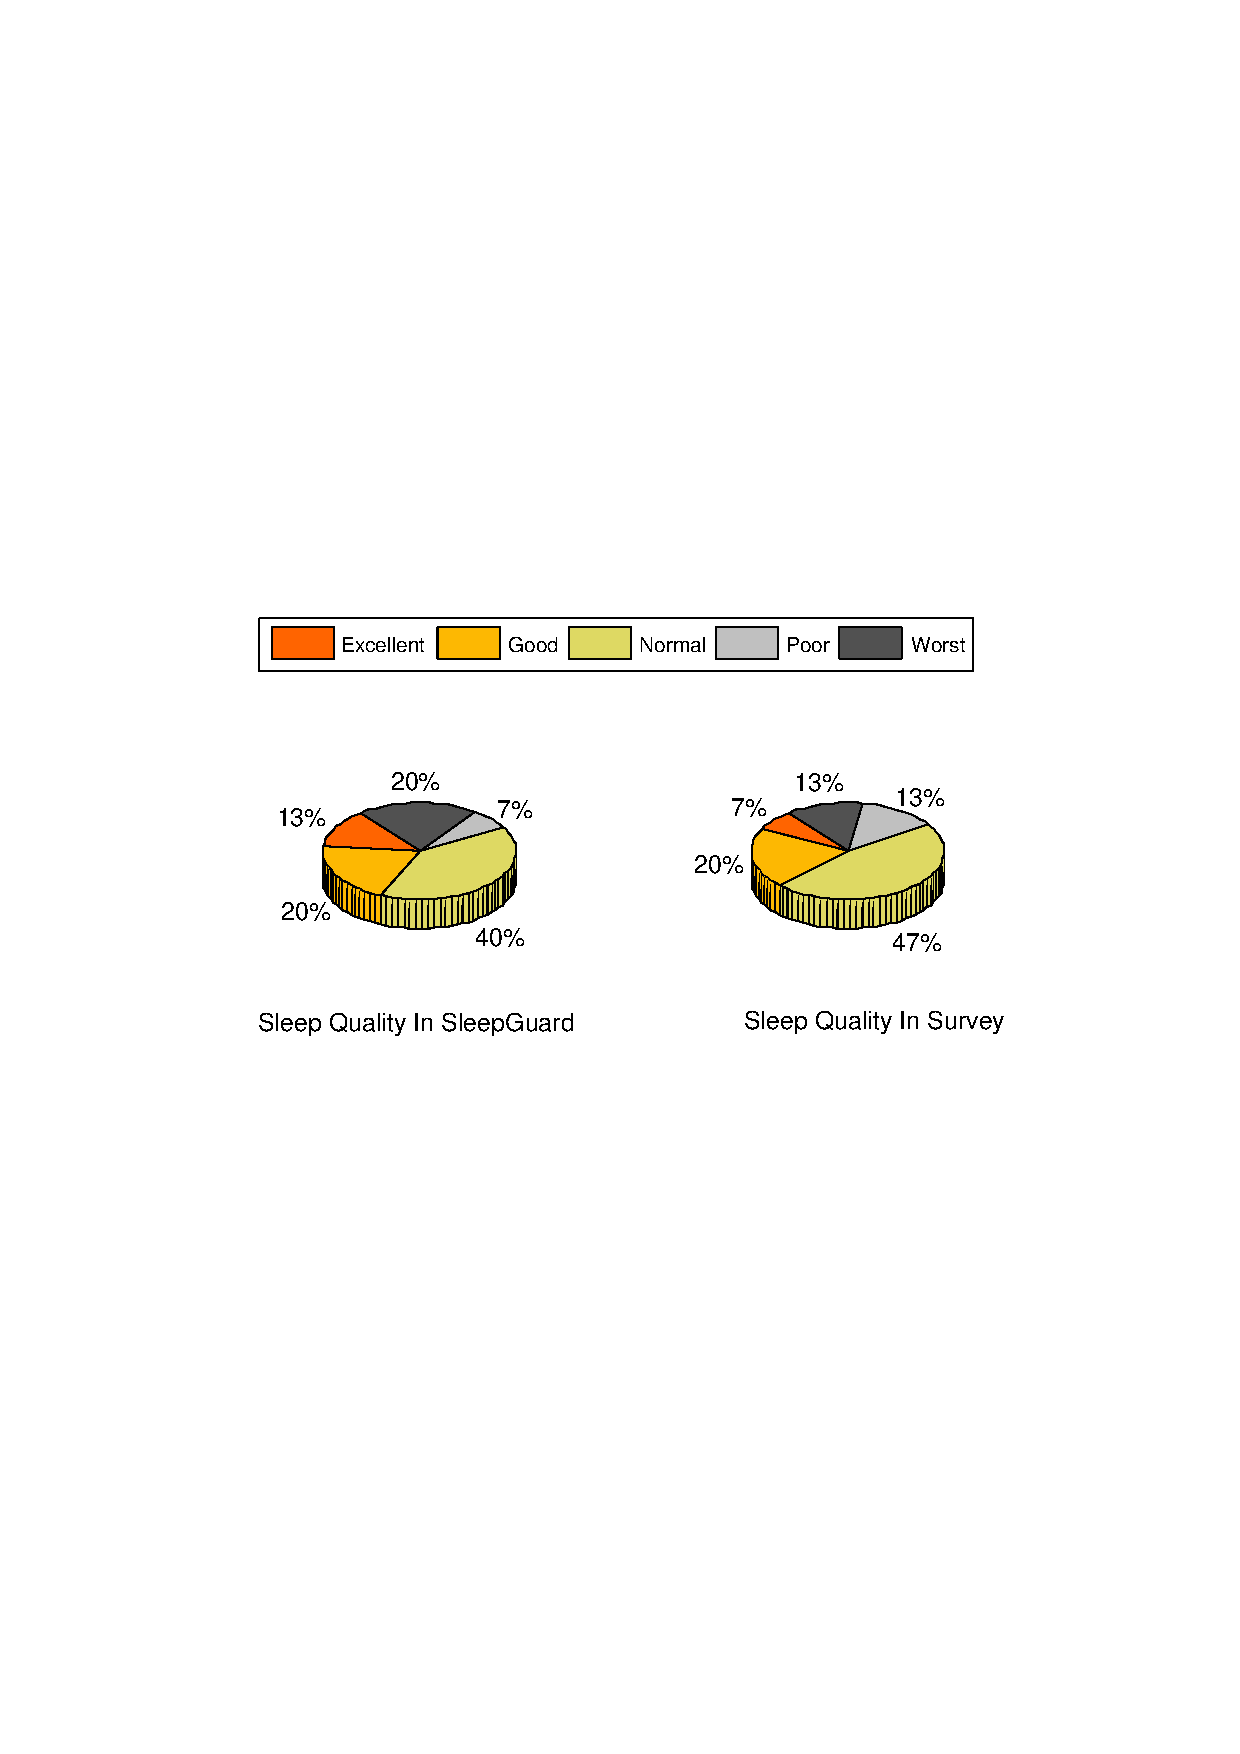
\includegraphics[width=0.52\linewidth]{Figures/quality.pdf}
 %\caption{Participants' sleep quality distribution}\label{fig:quality}
%\end{figure}

\section{DISCUSSION}\label{sec:discussion}

In this paper, we have shown that sensors available on off-the-shelf smartwatches can be used to capture rich information about sleep quality and factors affecting it. The main focus of our work has been to develop the required algorithms for capturing rich sleep related information as accurately as possible. While the recognition performance of our system is very encouraging, there are some issues that would need to be addressed in our system before larger-scale deployment would be feasible. Below we highlight the main issues and briefly discuss possible ways to overcome them.


%In this work, we try to examine the possibilities of using smart wearables to detect sleep. Our focus is to provide a series of ways to detect sleep-related events that will greatly assist in the assessment of sleep quality.While our results are satisfactory, there are still a handful of issues to address as we highlight below.

\begin{itemize}
  \item \textbf{The accuracy of sleep stage detection.}
  Compared with polysomnography-based sleep stage detection, the accuracy of {\systemname} is lower and it is rather difficult to achieve comparable performance. This is because polysomnography monitors and analyzes sleep based on information that directly correlates with sleep such as EEG, EMG, EOG, and oxygen saturation, whereas {\systemname} estimates sleep quality from cues that have have an indirect effect on sleep quality. In particular, \systemname only combines the body movement, acoustic events, sleep environment and other events during sleep to predict the sleep stage. Therefore, {\systemname} is not a replacement for professional medical equipment for high-precision sleep detection, but serves as a personal technology that provides easy-to-use and non-intrusive way to monitor personal sleep patterns and to obtain feedback about the, % However, SleepGuard is able to take advantage of the popularity of business smartwatches to provide easy-to-use and less intrusive sleep detection services, making it easy for users to learn about their sleep and make adjustments based on suggestions.
  \item \textbf{Battery life.} 
  A critical design requirement for sleep detection is that the monitoring can operate sufficiently long to cover the entire duration of the user's sleep. battery capacity on smartwatches is rather limited, resource consumption needs to be optimized by considering both the data collection and analysis phases. In our experiments we demonstrated that additional devices in the vicinity of the smartwatch can be taken advantage of, for example, some of the sensing and processing tasks can be offloaded to smartphones or other smart devices located within sufficient proximity. Particularly the acoustic event detection could be offloaded to smartphones that are located on the bedside table or elsewhere in the user's vicinity as smartphones increasingly integrate co-processors for audio processing that allow performing the audio event detection with a small energy footprint. We have also designed our analysis techniques to be as lightweight as possible to minimize energy consumption. Further improvements can be achieved by designing dynamic duty cycling strategies that reduce sampling during periods of regularity, and by using simple triggering mechanisms, such as a motion intensity detector to reduce processing overhead. Exploring these techniques is part of our future work.%For our work, we only use smartwatch as devices for data collection and delivery, while other computing capabilities are mainly implemented on smartphone, and we also have adopted simpler algorithms to reduce resource usage. But despite this, our smartwatch can only continue to collect about 6 hours of sensor data, which is not sufficient for longer sleep detection, so we still need to further study how to reduce power consumption. One possible solution is to change the data collection strategy to dynamically adjust the sampling frequency based on whether the body is moving or not.
  \item \textbf{Sensor data.}
  One limitation of {\systemname} is that we have not taken advantage of heart rate when determining the current sleep stage of the user. The main reason for this is programming limitations of the Huawai Smartwatch 2 device used in the experiments. Specifically, the device does not support querying heart rate information, but only provides it through a dedicated application. The output of this application is unfortunately not sufficiently accurate for sleep monitoring purposes, and restricts the rate at which information can be acquired. To compensate for the lack of heart rate data, \systemname considers the respiratory amplitude detected from accelerometer instead. As shown in our experiments, the respiratory amplitude detection significantly improves the performance of the sleep stage detection. % which can help us improve the performance of the sleep stage detection (it has been proved in our experiment).
  \item \textbf{Limitations of the algorithm.}
  When we try to detect sleep posture, we find a corresponding relationship between the position of the arm and the sleeping posture, so we indicate the sleeping posture by detecting its position. But currently we consider some specific positions of the arm in the four sleeping positions, some unusual arm's positions are ignored by us and that is something we need to improve further in future work.
\end{itemize}

\section{RELATED WORK}\label{sec:5related}

Sleep quality is a crucial issue for each individual, and the poor sleep would lead to numerous diseases, such as  endocrine dyscrasia, depression, immunity decline \cite{vgontzas2009insomnia,gottlieb2005association}. Thus, a lot of research works have been proposed to monitor the sleep \cite{langkvist2012sleep,hao2013isleep,bai2012will,kay2012lullaby,bain2003evaluation,pombo2016ubisleep}. Below, we summarize the related state-of-the-art research works as the following three categories.

\textbf{Medical technology based work}. Traditionally, the dedicated medical technologies, like EEG, ECG and EMG \cite{saper2005hypothalamic}, have been applied for sleep monitoring. Those technologies rely on the certain biomedical signals, such as brain wave, muscle tone and eye movement, to assess the sleep quality. For example, the EEG technology in \cite{langkvist2012sleep,oropesa1999sleep,ebrahimi2008automatic} monitors the brain waves, and then recognizes the sleep stages by leveraging unsupervised learning approaches.

Although a high accuracy achieved by those  technologies, they have two drawbacks. First, those  technologies require the dedicated medical devices, which are very expensive compared the widely available  smart watch/phone. Second, they require the users to be attached lots of sensors on the human body, which may cause a healthy person had to sleep and result in large errors.

Compared with those medical technologies, our system has two advantages. First, we only need a smartwatch, which is cost effective. Second, the smartwatch does not disturb a user's normal sleep, thus we can monitor the user's sleep quality more accurately.

\textbf{Smartphone based work}. Recently, some researches use the smartphones for sleep monitoring \cite{hao2013isleep,bai2012will,kay2012lullaby,choe2011opportunities} . iSleep \cite{hao2013isleep} measures the sleep quality by recording the sleep-related acoustic events and evaluates the sleep quality using the Pittsburgh Sleep Quality Index (PSQI) \cite{carpenter1998psychometric}. Bai et al. \cite{bai2012will} predicts a user's sleep quality by observing the user's daily activities with the smartphone's sensor data, like the accelerometer, gyroscope, microphone, etc. Work in \cite{kay2012lullaby} leverages the smartphone sensors to record the sleep disruptors for a user. The authors in \cite{choe2011opportunities}  explore a series of opportunities to support healthy sleep behaviors based on the smartphone sensors. Several research works predict the sleep quality by using the smartphone to monitor the external  influence  factors, such as the daily activity, sleeping environment, location and family settings \cite{chen2013unobtrusive,zhang2013real}. Besides those research works, many Smartphone Apps, such as Sleep As Android \cite{SleepAndroid}, Sleep Journal \cite{SleepJournal}, YawnLog \cite{YawnLog} also have been developed to monitor a uer's sleep quality.

Those smartphone based systems, however, require placing the smartphone at a specifically location near to the user, which usually cannot be satisfied in reality. For example, Gu et al. \cite{gu2016sleep} needs the smartphone to be placed next to the user's head, and requires the smartphone keeping stationary throughout the sleeping process. But, many users do not want to place the mobile phone too close to the body due to health risk concerns  \cite{StepHealth,Quorasleep}.

Compared with the existing smartphone based systems, our system uses the commodity smartwatch for sleep monitoring. Since many users are willing to wear the smartwatch throughout the night, thus the smartwatch can remain relatively close to the user over the duration of sleep. The smartwatch also allows us to collect a richer set of information, which enables a wider range of sleep-related events and more accurate to achieve sleep detection and sleep quality assessment.


\textbf{Smartwatch based work}. With the widely use of wearable devices, more and more researchers and industries try to  use the smartwatch or wearable-wrist for sleep monitoring \cite{bain2003evaluation,bonnet2003insomnia,pombo2016ubisleep,caviness1996myoclonus}.  The Sleeptracker
\cite{sleeptracker} is a wristwatch-shaped unit that apart from telling the time, also infers whether the user is in deep sleep, light sleep, or awake, using an accelerometer. The ubiSleep \cite{pombo2016ubisleep} joints heart rate, accelerometer, and sound signals collected into the smartwatch for noninvasive sleep monitoring. The aXbo alarm clock [9] is packaged as a stand-alone application in the form of an alarm clock that wirelessly communicates with a wrist-band unit. The Zeo \cite{caviness1996myoclonus} is similarly using an alarm clock base unit with a worn sensing device, but the latter is a headband rather than a wrist-band that based on electroencephalograph (EEG) to monitor sleep. We know Zeo has good performance in sleep stage detection compared to some wristband sleep monitoring products because products based on some biological signals like EEG are able to get more accurate and more representative sleep data than actigraphy-based \cite{Actigraphy} sleep monitoring products. However, the vast majority of biosignal-based sleep detection approaches require specialized equipment, which is high cost and complex to operate, while the approaches based on actigraphy are well adapted and user-friendly to accept and understand.

Moreover, these actigraphy-based wristband devices or smartwatch Apps only can gather coarse-grained information and  do not design a model for deep understanding the relationship between a user��s sleep pattern and the sensor data. For example, many smartwatch Apps, like Jawbone Up \cite{Jawbone}, FitBit \cite{fitbit}, YawnLog \cite{YawnLog} and WakeMate \cite{WakeMate}, do not show how they assess a user��s sleep quality based on what kind of sensor data.

Compared with the existing smartwatch or wearable-wrist based systems, our system can collect an extensive set of sleep-related events, many of which are not supported in prior work. Our system enables users to gain a deeper understanding of their sleep patterns and the causes of poor sleep.


\section{CONCLUSION}
This paper presents \systemname, a smartwatch based deep understanding of sleep detection system. \systemname exploits the rich sensor data
provided by smartwatches to track a wider range of sleep-related activities. To detect sleep related activities, we effectively exploit the
smartwatch sensor data and design a set of new algorithms based on the particular characteristics. Extensive experimental results show that
\systemname can accurately identify lots of sleep activities, including body postures, body rollover, hand positions and acoustical events.
In the future work, we will optimize the energy consumption and design detection models for more events.


\bibliographystyle{ACM-Reference-Format}
\bibliography{sleep_ref}

\end{document}
